%% For normal draft builds (figs undisplayed hence fast compile)
%\documentclass[hyperpdf,nobind,draft,oneside]{hepthesis}
%\documentclass[hyperpdf,nobind,draft,twoside]{hepthesis}

%% For short draft builds (breaks citations by necessity)
%\documentclass[hyperpdf,nobind,draft,hidefrontback]{hepthesis}
\documentclass[hyperpdf,oneside,bindnopdf,usenames,dvipsnames,svgnames,table,longbibliography]{hepthesis}

%%For Cambridge soft-bound version \documentclass[hyperpdf,bindnopdf,usenames,dvipsnames,svgnames,table]{hepthesis}
%% For Cambridge hard-bound version (must be one-sided)
%\documentclass[hyperpdf,oneside]{hepthesis}

%% Load special font packages here if you wish
%\usepackage{lmodern}
\usepackage{mathpazo}
\usepackage{multicol}
%\usepackage{euler}
\usepackage{lineno}
\usepackage{relsize}
\usepackage{subcaption}
\usepackage{caption}
\usepackage{verbatim}
\usepackage{atbegshi}
\usepackage{pdfpages}
%---------------Add line numbers--------------%
%\linenumbers
%---------------Add line numbers--------------%

%% Put package includes etc. into preamble.tex for convenience
\usepackage{xspace}
\usepackage{tikz}
\usepackage{morefloats,afterpage,subcaption}
\usepackage{mathrsfs} % script font
\usepackage{verbatim}

\usepackage{graphicx}
\usepackage{wrapfig}
\usepackage[rightcaption]{sidecap}
\usepackage{pgfgantt}
\usepackage{rotating}
%\usepackage[usenames,dvipsnames,svgnames,table]{xcolor}
\usepackage{xcolor}


%% Using Babel allows other languages to be used and mixed-in easily
%\usepackage[ngerman,english]{babel}
\usepackage[english]{babel}
\selectlanguage{english}

%% Citation system tweaks
\usepackage{cite}
% \let\@OldCite\cite
% \renewcommand{\cite}[1]{\mbox{\!\!\!\@OldCite{#1}}}

%% Maths
% TODO: rework or eliminate maybemath
\usepackage{abmath}
\DeclareRobustCommand{\mymath}[1]{\ensuremath{\maybebmsf{#1}}}
% \DeclareRobustCommand{\parenths}[1]{\mymath{\left({#1}\right)}\xspace}
% \DeclareRobustCommand{\braces}[1]{\mymath{\left\{{#1}\right\}}\xspace}
% \DeclareRobustCommand{\angles}[1]{\mymath{\left\langle{#1}\right\rangle}\xspace}
% \DeclareRobustCommand{\sqbracs}[1]{\mymath{\left[{#1}\right]}\xspace}
% \DeclareRobustCommand{\mods}[1]{\mymath{\left\lvert{#1}\right\rvert}\xspace}
% \DeclareRobustCommand{\modsq}[1]{\mymath{\mods{#1}^2}\xspace}
% \DeclareRobustCommand{\dblmods}[1]{\mymath{\left\lVert{#1}\right\rVert}\xspace}
% \DeclareRobustCommand{\expOf}[1]{\mymath{\exp{\!\parenths{#1}}}\xspace}
% \DeclareRobustCommand{\eexp}[1]{\mymath{e^{#1}}\xspace}
% \DeclareRobustCommand{\plusquad}{\mymath{\oplus}\xspace}
% \DeclareRobustCommand{\logOf}[1]{\mymath{\log\!\parenths{#1}}\xspace}
% \DeclareRobustCommand{\lnOf}[1]{\mymath{\ln\!\parenths{#1}}\xspace}
% \DeclareRobustCommand{\ofOrder}[1]{\mymath{\mathcal{O}\parenths{#1}}\xspace}
% \DeclareRobustCommand{\SOgroup}[1]{\mymath{\mathup{SO}\parenths{#1}}\xspace}
% \DeclareRobustCommand{\SUgroup}[1]{\mymath{\mathup{SU}\parenths{#1}}\xspace}
% \DeclareRobustCommand{\Ugroup}[1]{\mymath{\mathup{U}\parenths{#1}}\xspace}
% \DeclareRobustCommand{\I}[1]{\mymath{\mathrm{i}}\xspace}
% \DeclareRobustCommand{\colvector}[1]{\mymath{\begin{pmatrix}#1\end{pmatrix}}\xspace}
\DeclareRobustCommand{\Rate}{\mymath{\Gamma}\xspace}
\DeclareRobustCommand{\RateOf}[1]{\mymath{\Gamma}\parenths{#1}\xspace}

%% High-energy physics stuff
\usepackage{abhep}
\usepackage{hepnames}
\usepackage{hepunits}
\DeclareRobustCommand{\arXivCode}[1]{arXiv:#1}
\DeclareRobustCommand{\CP}{\ensuremath{\mathcal{CP}}\xspace}
\DeclareRobustCommand{\CPviolation}{\CP-violation\xspace}
\DeclareRobustCommand{\CPv}{\CPviolation}
\DeclareRobustCommand{\LHCb}{LHCb\xspace}
\DeclareRobustCommand{\LHC}{LHC\xspace}
\DeclareRobustCommand{\LEP}{LEP\xspace}
\DeclareRobustCommand{\CERN}{CERN\xspace}
\DeclareRobustCommand{\bphysics}{\Pbottom-physics\xspace}
\DeclareRobustCommand{\bhadron}{\Pbottom-hadron\xspace}
\DeclareRobustCommand{\Bmeson}{\PB-meson\xspace}
\DeclareRobustCommand{\bbaryon}{\Pbottom-baryon\xspace}
\DeclareRobustCommand{\Bdecay}{\PB-decay\xspace}
\DeclareRobustCommand{\bdecay}{\Pbottom-decay\xspace}
\DeclareRobustCommand{\BToKPi}{\HepProcess{ \PB \to \PK \Ppi }\xspace}
\DeclareRobustCommand{\BToPiPi}{\HepProcess{ \PB \to \Ppi \Ppi }\xspace}
\DeclareRobustCommand{\BToKK}{\HepProcess{ \PB \to \PK \PK }\xspace}
\DeclareRobustCommand{\BToRhoPi}{\HepProcess{ \PB \to \Prho \Ppi }\xspace}
\DeclareRobustCommand{\BToRhoRho}{\HepProcess{ \PB \to \Prho \Prho }\xspace}
\DeclareRobustCommand{\X}{\thesismath{X}\xspace}
\DeclareRobustCommand{\Xbar}{\thesismath{\overline{X}}\xspace}
\DeclareRobustCommand{\Xzero}{\HepGenParticle{X}{}{0}\xspace}
\DeclareRobustCommand{\Xzerobar}{\HepGenAntiParticle{X}{}{0}\xspace}
\DeclareRobustCommand{\epluseminus}{\Ppositron\!\Pelectron\xspace}
\DeclareRobustCommand{\protonproton}{\Pproton\APantiproton\xspace}


% su style guidelines
% http://www.syr.edu/gradschool/em/pdfs/emdissertation/Doctoral%20Dissertation%20%20Masters%20theses%20Format%20Guidelines.pdf
% https://en.wikipedia.org/wiki/Book_design

%\usepackage[T1]{fontenc}

\usepackage{ifthen}

\newboolean{isdraft}
\setboolean{isdraft}{true} % change to false when final version is ready

\usepackage{adjustbox} % for clipping seal images in xelatex
\usepackage{rotating} % for sidewaysfigure

%\usepackage[tracking=true]{microtype}
%\SetTracking
% [ no ligatures = {f},
% spacing = {600*,-100*, },
% outer spacing = {450,250,150},
% outer kerning = {*,*} ]
% { encoding = * }
% { 160 }
\newcommand\tracked[1]{\textls{#1}}

% if using xelatex, will also format math
%\usepackage[Numbers=OldStyle,Ligatures=TeX,Scale=MatchLowercase]{mathspec}
%\setallmainfonts{Source Sans Pro Light}
%\newfontfamily\semibold{Source Sans Pro}
%\newcommand\tracked[1]{{\addfontfeature{LetterSpace=12}#1}} % for all caps words
%\usepackage{xunicode}
%\defaultfontfeatures{Mapping=tex-text}
%\usepackage{unicode-math}
%\usepackage{hvmath}
%\usepackage[Euler]{upgreek}







\usepackage{floatrow}
% Table float box with bottom caption, box width adjusted to content
\newfloatcommand{capbtabbox}{table}[][\FBwidth]
\usepackage{array}

\newenvironment{conditions}
  {\par\vspace{\abovedisplayskip}\noindent\begin{tabular}{>{$}l<{$} @{${}={}$} l}}
  {\end{tabular}\par\vspace{\belowdisplayskip}}

\newcommand{\mc}[2]{\multicolumn{#1}{c}{#2}}
\definecolor{Gray}{gray}{0.85}
\definecolor{LightCyan}{rgb}{0.8,1,1}
\newcolumntype{a}{>{\columncolor{LightCyan}}c}
%% You can set the line spacing this way
%\setallspacing{double}
%% or a section at a time like this
%\setfrontmatterspacing{double}



%% Doc-specific PDF metadata
\makeatletter
\@ifpackageloaded{hyperref}{%
\hypersetup{%
  pdftitle = {$\mu/\pi$ separation using Convolutional Neural Networks for the MicroBooNE Charged Current Inclusive Cross Section Measurement},
  pdfsubject = {Jessica Esquivel's P.hD Thesis},
  pdfkeywords = {MicroBooNE, CC-Inclusive, physics, FNAL, CNN},
  pdfauthor = {\textcopyright\ Jessica Esquivel}
}}{}
\makeatother

%\AtBeginDocument{\AtBeginShipoutNext{\AtBeginShipoutDiscard}}

%% Start the document
\begin{document}

\begin{frontmatter}

  \thispagestyle{empty}
  \let\cleardoublepage\clearpage
\begin{abstract}%[\smaller \thetitle\\ \vspace*{1cm} \smaller {\theauthor}]
  \thispagestyle{empty}
The purpose of this thesis was to use Convolutional Neural Networks (CNN) to separate $\mu'{s}$ and $\pi'{s}$ for use in increasing the acceptance rate of $\mu'{s}$ below the implemented 75cm track length cut in the Charged Current Inclusive (CC-Inclusive) event selection for the CC-Inclusive Cross-Section Measurement. In doing this, we increase acceptance rate for CC-Inclusive events below a specific momentum range.
\end{abstract}
\let\cleardoublepage\clearpage
\newpage

\begin{center}
\vspace*{0.2cm}
\noindent\makebox[\linewidth]{\rule{\textwidth}{0.3pt}}
{\huge %[Update Title]\\
$\mu/\pi$ separation using \\Convolutional Neural Networks for the \\MicroBooNE Charged Current Inclusive \\Cross Section Measurement 
%Muon/Pion separation using Convolutional Neural Networks for the MicroBooNE Charged Current Inclusive Cross Section Measurement 
%Put in your Title\\[-0.3cm]
%in titlepage.tex\\[0.4cm]
}
\noindent\makebox[\linewidth]{\rule{\textwidth}{0.3pt}}\\ % fix spacing here
\vspace{0.5cm}
%by (fix spacing above and at top)\\
\vspace{0.6cm}
\tracked{\large Jessica Nicole Esquivel}\\[6pt]
B.S., Saint Mary's University, 2011\\
\vspace{1.6cm}
\tracked{\large DISSERTATION}\\[6pt]
Submitted in partial fulfillment\\
of the requirements for the degree\\
\emph{Doctor of Philosophy in Physics}\\

\ifthenelse{\boolean{isdraft}}{
\vspace{1.5cm}
- * - \tracked{DRAFT \today}~- * -\\[0.5cm]
}
{
\vspace{1.5cm}
}
SYRACUSE UNIVERSITY\\ 
May, 2018\\

\end{center}
%\setcounter{page}{2}
\thispagestyle{empty}
%\clearpage
\let\cleardoublepage\clearpage

\vspace*{8cm}
\begin{center}
    Copyright $\textsuperscript{\textcopyright}$ Jessica Nicole Esquivel\\
    2018\\
    All Rights Reserved\\
\end{center}
\thispagestyle{empty}
\let\cleardoublepage\clearpage

% 
\vspace*{1cm}
\begin{center}
\adjustbox{height=3cm,width=.2\textwidth, trim=0mm 20mm 0mm 0mm,clip}{
\includegraphics[scale=1.3]{figs/seal_bw2}}
\includegraphics[scale=.3]{figs/uboone.png}
\includegraphics[scale=.15]{figs/nsf2.pdf}\\[10pt] % use trim=l b r t,clip=true to get rid of the bottom white space, trim doesn't work in xelatex
%\adjustbox{height=3cm,width=.2\textwidth, trim=0mm 0mm 12mm 80mm,clip}{}\\[10pt] % also trim this one
\end{center}
%\thispagestyle{empty}

\clearpage

%% Define the un-numbered front matter (cover pages, rubrik and table of contents)
  %\end{titlepage% Title
%\titlepage[of Syracuse University]{%
%  A dissertation submitted to  Syracuse University\\ for the degree of Doctor of Philosophy}

%% Declaration
\begin{declaration}
%\setcounter{page}{4}
  I dedicate this dissertation to the two most important women in my life; my mom and my wife. Mom, you taught me how to stand up for myself, how to trust in my abilities, and that hard work always pays off. Em, you've been and continue to be my rock, steadying me as I questioned whether or not I could do this, loving me through all the late nights and keeping me sane. Both have been there cheering me on giving me strength and love as I worked towards the hardest thing I've ever accomplished.  

  \vspace*{1cm}
  \begin{flushright}
    Jessica Nicole Esquivel 
  \end{flushright}
\end{declaration}


%\vspace*{1cm}
%\begin{center} % use InkScape to edit these, if necessary.
%\setlength\fboxsep{0pt} % use fbox to see the extra space around graphics
%\setlength\fboxrule{0.5pt} % remove when done
%\fbox{\includegraphics{chick}}
%\adjustbox{height=3cm,trim=0mm 20mm 0mm 0mm,clip}{
\includegraphics{figs/seal_bw2}}\\[20pt] % use trim=l b r t,clip=true to get rid of the bottom white space, trim doesn't work in xelatex
%
\includegraphics[height=3cm]{figs/lhcb-logo2}\\[20pt] % this one is good, no trimming
%\includegraphics[height=3cm]{figs/LHC-logo}\\[10pt]
%
\includegraphics[height=3cm]{figs/cern_logo}\\[20pt]  % this one is good, no trimming
%\adjustbox{height=3cm,trim=0mm 0mm 12mm 80mm,clip}{
\includegraphics{figs/nsf2.pdf}}\\[10pt] % also trim this one
%\end{center}
%\thispagestyle{empty}

%\clearpage
%% Acknowledgements
\begin{acknowledgements}
%\setcounter{page}{5}
  Of the many people who deserve thanks, some are particularly prominent,
  such as my advisor Mitch Soderberg who took a chance on me and supported me even though I struggled through the courses. Katherine, thanks for always lending an ear to bounce off ideas, answering all my questions and for being my best friend. Duncan Brown, thank you for seeing that there was potential in me and for helping me get through the hurdle that was Quals. Fabian, thank you for studying for the Quals with me. Without your infectious optimism I wouldn't have made it. To Richard Cardenas, thanks for being the first person to introduce me to physics as a career choice and for supporting me when no one believed I could double major in Electrical Engineering and Applied Physics in 4 years. Lastly, thank you Jedidah Isler for showing me that it is possible for a woman of color to succeed in this field and for taking a vested interest in my success.     
\end{acknowledgements}


%% Preface
%\begin{preface}
%  This thesis describes my research on various aspects of the \LHCb
%  particle physics program, centred around the \LHCb detector and \LHC
%  accelerator at \CERN in Geneva.

%  \noindent
%  For this example, I'll just mention \ChapterRef{chap:SomeStuff}
%  and \ChapterRef{chap:MoreStuff}.
%\end{preface}

%% ToC
\addtocontents{toc}{\protect{\pdfbookmark[0]{\contentsname}{toc}}}
%\tableofcontents
%\listoffigures
%\listoftables
%{\tableofcontents \let\cleardoublepage\clearpage \listoffigures \let\cleardoublepage\clearpage \listoftables}
{\tableofcontents \listoffigures \listoftables}

%% Strictly optional!
\frontquote{%
  If they don't give you a seat at the table, \\
  bring a folding chair.}%
  {Shirley Chisholm}
%% I don't want a page number on the following blank page either.
\thispagestyle{empty}

\end{frontmatter}
%\setcounter{page}{6}

%% Start the content body of the thesis
\begin{mainmatter}
  %% Actually, more semantic chapter filenames are better, like "chap-bgtheory.tex"
  % perhaps put introduction in the front matter
% and have three chapters of 1) current understanding
%                            2) experimental considerations
%                            3) theoretical motivation
% decide later, do the writing first
\chapter{Introduction}
%\addcontentsline{toc}{chapter}{Introduction}
This thesis will be a description of work done to further increase effiiciency and purity of the charged current inclusive cross section measurement using the MicroBooNE detector. It will also describe the MicroBooNE detector, what neutrinos are, the charged current inclusive cross section measuremnt and it's importance as well as convolutional neural networks and how they can be used in $\mu/\pi$ separation. 
Chapter \ref{ch:neutrinos} will talk about the background of neutrinos and the people and detectors that discovered neutrinos as well as an in depth history of neutrino oscillation and the discovery that neutrinos have mass. 
Chapter \ref{ch:micriboone} will discuss the MicroBooNE experiement, specifically,  how Liquid Argon Time Projection Chambers work, the Light Collection System and the Electronic and Readout Trigger systems.
Chapter \ref{ch:beam} will describe the Booster Neutrino Beam sationed at Fermi National Accelerator Lab. It will go into depth on the neutrino flux and \dots
Chapter \ref{ch:neutrinoID} will discuss the work I did on detecting the first neutrinos seen in the MicroBooNE detector and the software reconstruction efforts required to create an automated neutrino ID filter that was used to find the first neutrinos and then was later expanded on to create the charged current inclusive filter that will be discussed in chapter \ref{ch:meas}
Chapter \ref{ch:mupi} will discuss the importance of $\mu/\pi$ separation for the charged current inclusive cross section measurement.
Chapter \ref{ch:cnn} will give a brief description of what Convolutional Neural Networks are and how it will be used for $\mu/\pi$ separation in this selection. 
Chapter \ref{ch:hardware} will discuss hardware
Chapters \ref{ch:cnn_results}, \ref{ch:data} and \ref{ch:selImodcompare} will discuss the results of using Convolutional Neural Networks on monte-carlo and data to sift out charged current inclusive neutrino events. 

  \chapter{Neutrinos}\label{ch:neutrinos}
%\addcontentsline{toc}{chapter}{Neutrinos}

\section{What are Neutrinos}
Neutrinos are fundamental particles which help make up the universe. They are also one of the least understood. Neutrinos are not affected by the electromagnetic force because they do not have electric charge. Neutrinos are affected by a weak sub-atomic force of much shorter range than electromagnetism, and are therefore able to pass through great distances in matter without much possibility of being affected by it. Until the late 1990's, neutrinos were thought to have no mass. Neutrinos are created by radioactive decay such as the ones that happen in the sun, in nuclear reactors or when cosmic rays hit atoms. There are three types of neutrinos, $\nu_{e}$, $\nu_{\mu}$ and $\nu_{\tau}$ which correspond to their charged lepton pairs.  

As previously stated, neutrinos are very weakly interacting; in fact, neutrinos can pass unscathed through a wall of lead several hundred light-years thick. Because neutrinos interact so rarely, studying neutrinos requires a massive detector and a powerful neutrino source. With that being said, we can only ``see'' a neutrino when they interact in a detector. In a collision, distinct charged particles are produced with each type of neutrino because of the weak force. An electron neutrino will create an electron, a muon neutrino will create a muon, and a tau neutrino will create a tau. The charged lepton track the particle leaves in the detector is how one figures out what type of neutrino interaction was ``seen''. Liquid Argon Time Projection Chambers are being used to study neutrinos due to their excellent imaging and particle identification capabilities. 

\section{History of Neutrinos}
The neutrino was first postulated by Wolfgang Pauli in 1930 to explain how to resolve the conservation of energy, momentum and angular momentum problem in beta decay \cite{pauli}. Pauli suggested that this missing energy might be carried off, unseen, by a neutral particle (he called neutron) which was escaping detection. James Chadwick discovered a much heavier nuclear particle in 1932 that he also named neutron \cite{chadwick}, leaving two particles with the same name. Enrico Fermi was the first person to coin the term neutrino (which means little neutral one in Italian) in 1933 to fix this confusion. 

Fermi's paper \cite{fermi}, which was published in 1934, unified Pauli's neutrino with Paul Dirac's positron and Werner Heisenberg's neutron-proton model and his theory accurately explained many experimentally observed results. Wang Ganchang first proposed the use of beta capture to experimentally detect neutrinos and in 1956 Clyde Cowan and Frederick Reines published their work stating that they had detected the neutrino \cite{cowan1}\cite{cowan2}. The experiment called for anti-neutrinos created in a nuclear reactor by beta decay that reacted with protons producing neutrons and positrons: $\nu_{e} +p^{+}\rightarrow n^{0} + e^{+}$. Once this happens, the positron finds an electron and they annihilate each other and the resulting gamma rays are detectable. The neutron is detected by neutron capture and the releasing of another gamma ray. 

In 1962 Leon M. Lederman, Melvin Schwartz and Jack Steinberger were the first to detect interactions of the muon neutrino \cite{leonlederman}. The trio received the 1988 Nobel Prize in Physics for their discovery of the muon neutrino. The experiment used a beam of energetic protons from Brookhaven's Alternating Gradient Synchrotron (AGS) to produce a shower of pions. These pions would then travel 70 ft. towards a 5,000 ton steel wall. The pions then decayed into muons and neutrinos, the neutrinos being the only particle making it through. These neutrinos would enter a neon-filled detector producing muon spark trails that were detected and photographed, proving the existence of muon neutrinos. The experiment's use of the first ever neutrino beam was pioneering work that scientists around the world still use today.  

The first detection of the tau neutrino was announced in the summer of 2000 by the DONUT collaboration at Fermilab \cite{donut}.The scientists used the Tevatron to produce an intense neutrino beam. The neutrinos then passed through layers of nuclear emulsion. When a neutrino interaction would occur, charged particles would leave visible tracks in the emulsion. 

\subsection{Solar Oscillations and the Solar Neutrino Problem}

In the late 1960s, it was found that the number of electron neutrinos arriving from the sun was around $1/3$ to $1/2$ the number predicted by the Standard Solar Model. This became known as the solar neutrino problem \cite{bahcall1} and remained unresolved for around thirty years. This problem was resolved by the discovery of neutrino oscillation and mass \cite{neutrinooscillation1}-\cite{neutrinooscillation4}.

The standard solar model (SSM) is a mathematical model developed by John Bahcall of the sun as a spherical ball of gas with varying states of ionization.The solar neutrino flux derived from the SSM is shown in figure \ref{fig:solarmodel} \cite{bahcall2}. Nuclear fusion and decay processes produce an abundant amount of neutrinos. The standard solar model predicts that these reactions produce several groups of neutrinos, each with differing fluxes and energy spectra. The figure also shows the ranges of detection of existing solar neutrino experiments in different shades of blue to illustrate that they sample different portions of the solar neutrino energy spectrum. Three of these experiments are discussed below.

\begin{figure}[htp]
\centering
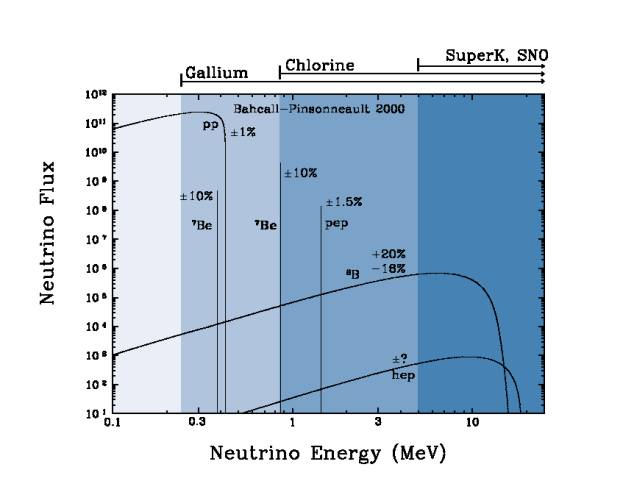
\includegraphics[scale=.55]{figs/solarmodel.jpg}
\captionof{figure}{The Standard Solar Model \cite{bahcall2}}
\label{fig:solarmodel}
\end{figure}

The first experiment to detect the effects of neutrino oscillation was Ray Davis's Homestake Experiment \cite{raydavis}. The detector was stationed in the Homestake Gold Mine in Lead, South Dakota. It was 1,478 meters underground and was 380 $\text{m}^3$. The detector was filled with perchloroethylene. Perchloroethylene was chosen because of its high concentrations of chlorine. When an $\nu_{e}$ interacted with a chlorine-37 atom, the atom would transform to argon-37 which was then extracted and counted. The neutrino capture reaction is shown in equation \ref{eq:capture}. Davis observed a deficit of about $1/3$ the flux of solar neutrinos that was predicted by Bahcall's Standard Solar Model. The unexplained difference between the measured solar neutrino flux and model predictions led to the Solar Neutrino Problem.

\begin{equation}
\label{eq:capture}
\nu_{e} +{}^{37}Cl \rightarrow {}^{37}Ar + e^{-}
\end{equation}

While it is now known that the Homestake Experiment results were indicating neutrino flavor oscillation, some physicists were weary of the results. Conclusive evidence of the Solar Neutrino Problem was provided by the Kamiokande-II experiment \cite{kamiokande}, a water cherenkov detector with a low enough energy threshold to detect neutrinos through neutrino-electron elastic scattering. In the elastic scattering interaction the electrons coming out of the point of reaction strongly point in the direction that the neutrino was traveling, away from the sun. While the neutrinos observed in Kamiokande-II were clearly from the sun, there was still a discrepancy between Kamiokande-II and Homestake; The Kamiokande-II experiment measured about 1/2 the predicted flux, rather than the 1/3 that the Homestake Experiment saw.

The solution to the solar neutrino problem was finally experimentally determined by the Sudbury Neutrino Observatory(SNO). Ray Davis's Homestake Experiment was only sensitive to electron neutrinos, and the Kamiokande-II Experiment was dominated by the electron neutrino signal. The SNO experiment had the capability to see all three neutrino flavors. Because of this, it was possible to measure the electron neutrinos and total neutrino flux. The experiment demonstrated that the deficit was due to the Mikheyev-Smirnov-Wolfenstein (MSW) effect \cite{Smirnov:2003da}, the conversion of electron neutrinos from their pure flavor state into the second neutrino mass eigenstate as they passed through a resonance due to the changing density of the sun. The resonance is energy dependent, and is visible near 2 MeV. The water cherenkov detectors only detect neutrinos above about 5 MeV, while the radiochemical experiments were sensitive to lower energy (0.8 MeV for chlorine, 0.2 MeV for gallium), and this turned out to be the source of the difference in the observed neutrino rates at the two types of experiments. Figure \ref{fig:solarexperiments} shows Homestake, Kamiokande-II and SNO experiments. 
\begin{figure}[htp]
\centering
	\begin{subfigure}[b]{.3\textwidth}
    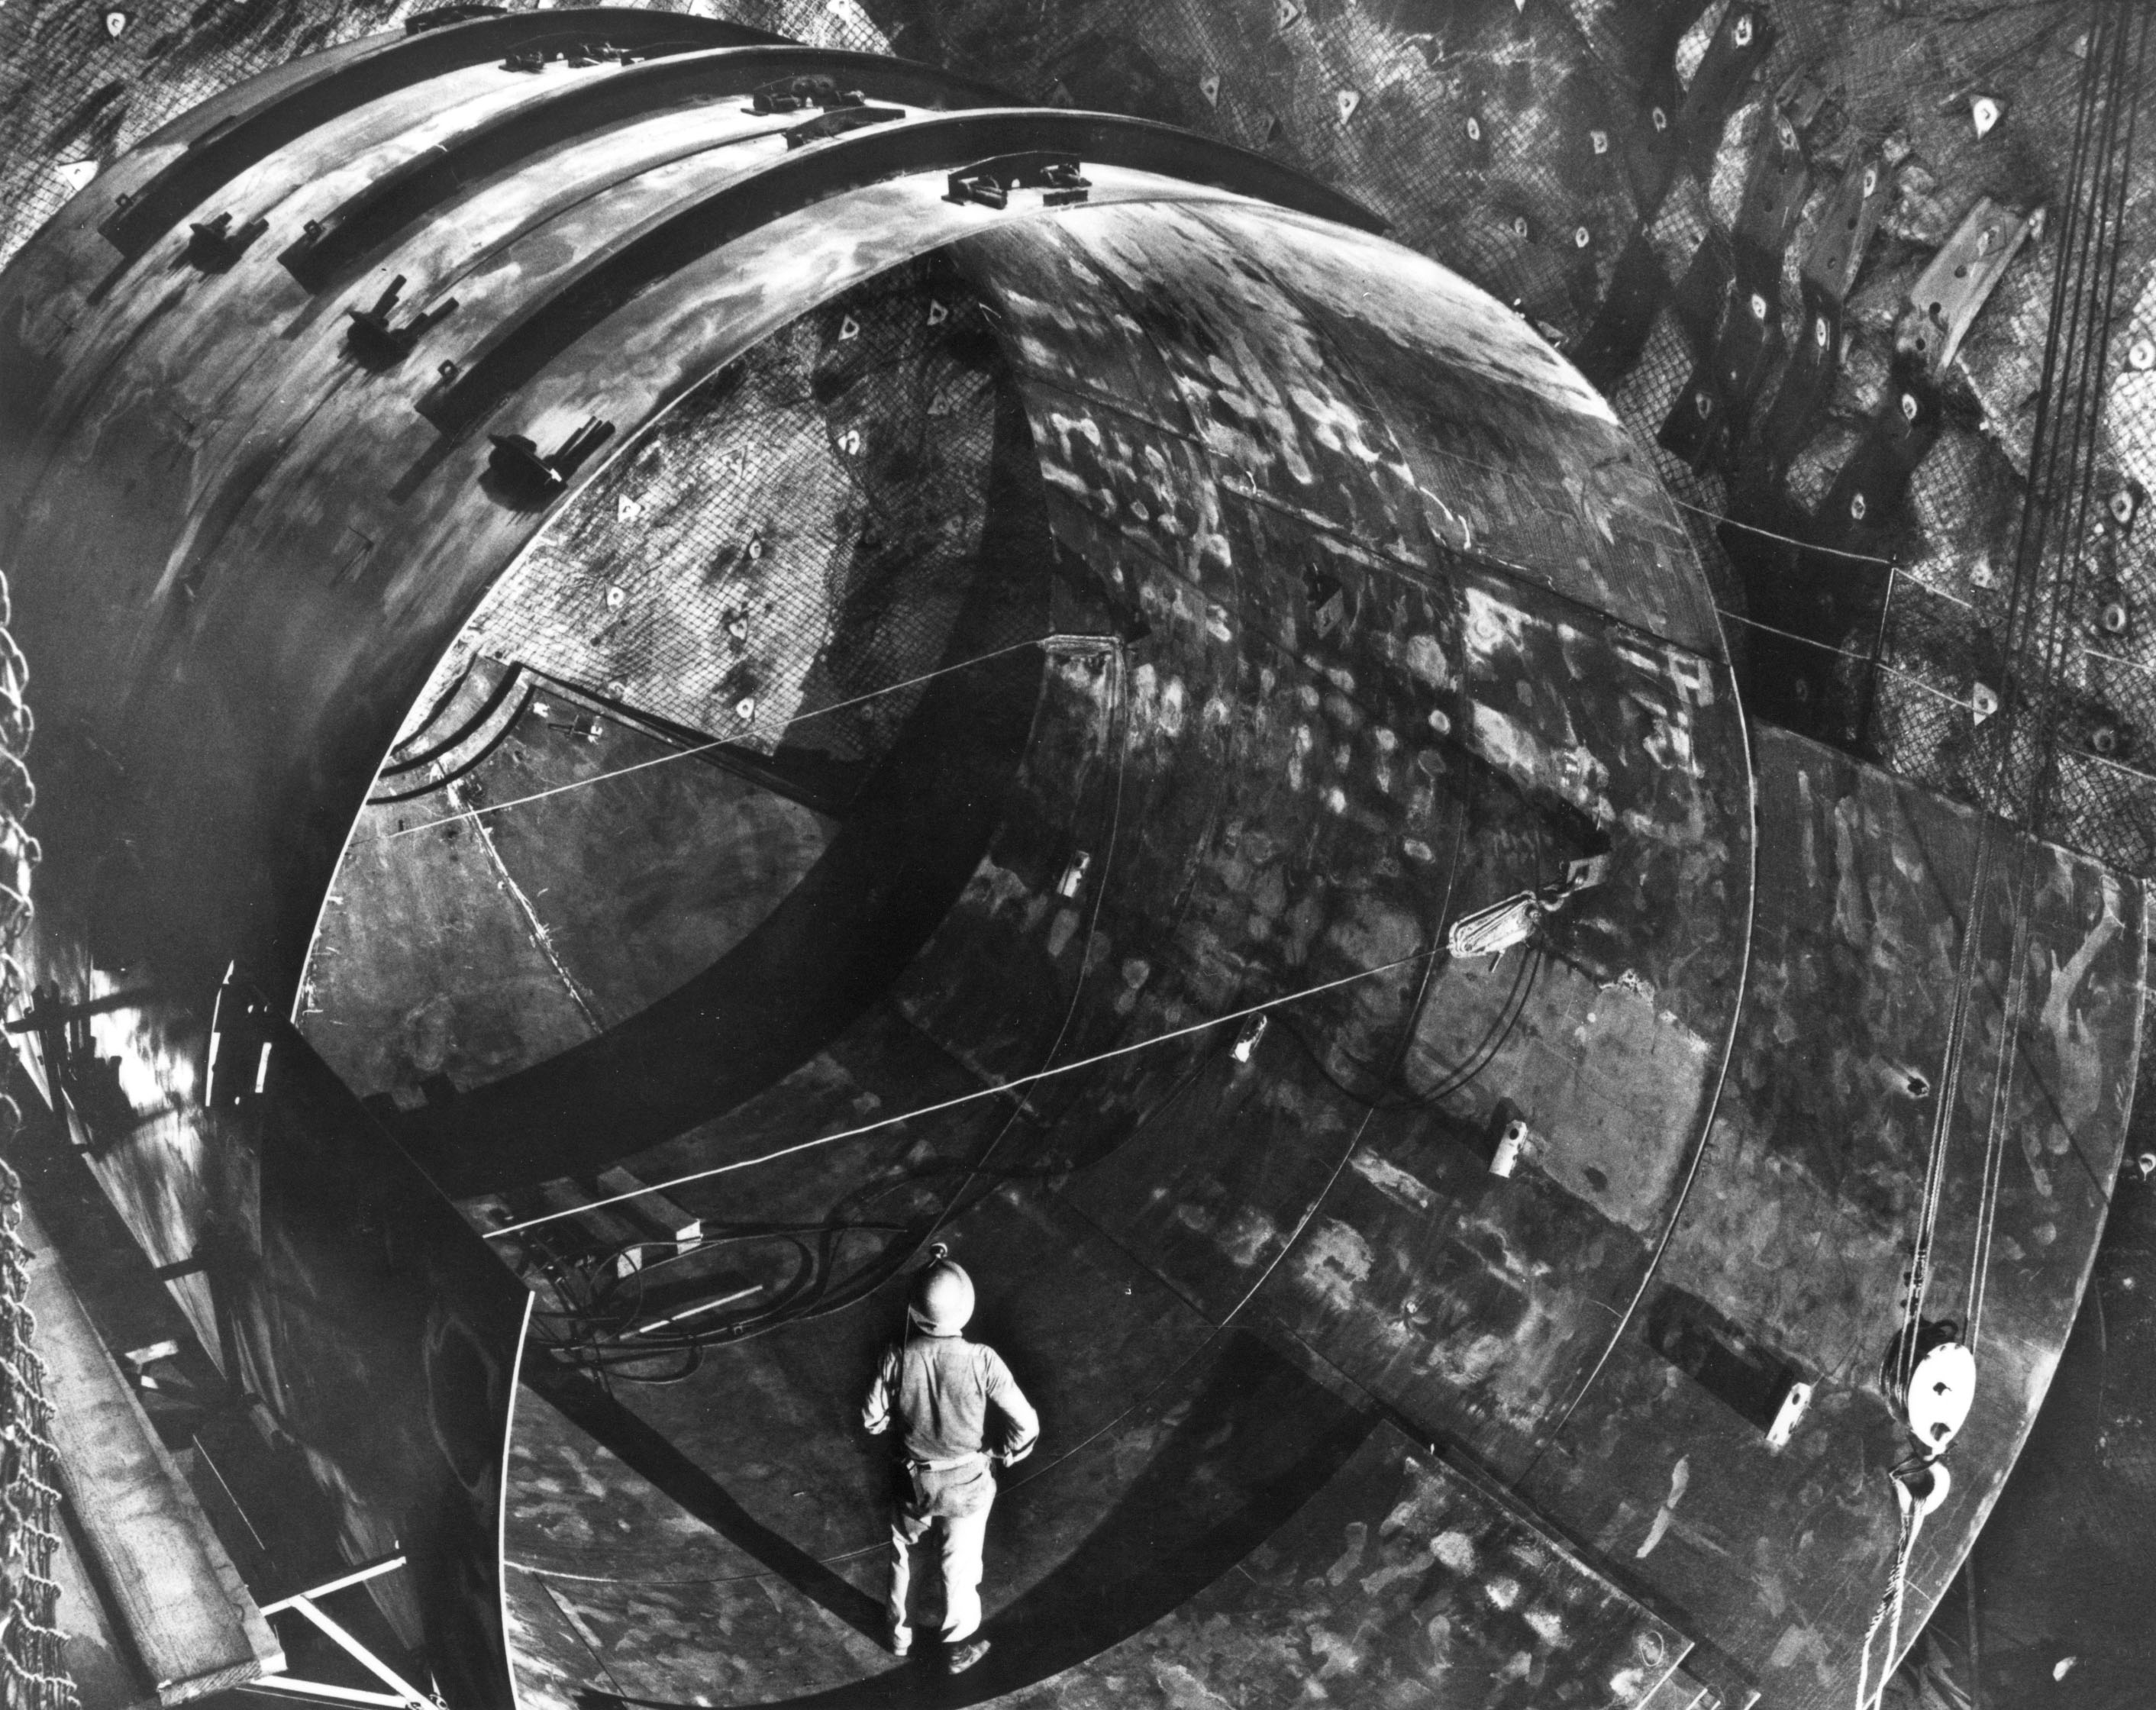
\includegraphics[width=\textwidth]{figs/homestake.jpg}
    \caption{Ray Davis's Homestake Experiment \cite{raydavis}}
    \label{fig:homestake}
    \end{subfigure}
    \quad
    \begin{subfigure}[b]{.3\textwidth}
    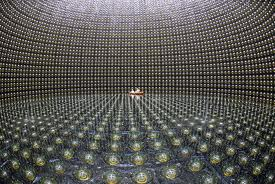
\includegraphics[width=\textwidth]{figs/kamiokande.jpg}
    \caption{Kamiokande-II Experiment \cite{kamiokande}}
    \label{fig:kamiokande}
    \end{subfigure}
    \quad
    \begin{subfigure}[b]{.3\textwidth}
    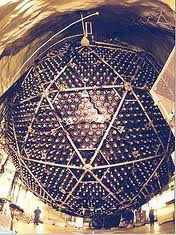
\includegraphics[width=\textwidth]{figs/sno.jpg}
    \caption{SNO Experiment \cite{Smirnov:2003da}}
    \label{fig:sno}
    \end{subfigure}
\caption{Solar Neutrino Experiments}
\label{fig:solarexperiments}
\end{figure}

%\subsubsection{MSW Effect}
%The Mikheyev-Smirnov-WOlfenshein effect is a process which acts to modify neutrino oscillations in matter. The presence of electrons in matter changes the energy levels of the mass eigenstates of neutrinos due to charged current coherent forward scattering of the electron neutrinos. This coherent forward scattering is similar to the electromagnetic process with respect to the refractive index of light in a medium. Because of this MSW Effect, neutrinos in vacuum have a different effective mass than neutrinos in matter and because neutrino oscillations depend on the squared mass difference of the neutrinos, the neutrino oscillations are different in matter than in vacuum. This effect is important at the sun where electron neutrinos are produced. The neutrinos of high energy leaving the sun are in a vacuum propagation eigenstate $\nu_{2}$ that has a very small overlap with the electron neutrino $\nu_{e}=\nu_{1}cos(\theta)+\nu_{2}sin(\theta)$ seen by the charged current reactions in Kamiokande-II and SNO. The discrepancy of the deficit between SNO, Kamiokande-II and Homestake is due to the energy of the solar neutrinos. The MSW effect "turns on" at about 2 MeV and at lower energies, this MSW effect is negligible. \cite{Smirnov:2003da}

\subsection{Atmospheric Oscillations and the Atmospheric Neutrino Anomaly}
Atmospheric neutrinos are neutrinos that stem from the decay hadrons coming from primary cosmic rays. The dominant part of the decay chain is shown in equations  \ref{eq:piplus} and \ref{eq:piminus}

\begin{equation}
\label{eq:piplus}
\pi^{+} \rightarrow \mu^{+} \nu_{\mu} \mu^{+} \rightarrow e^{+} \nu_{e} \overline{\nu_{\mu}}
\end{equation}
\begin{equation}
\label{eq:piminus}
\pi^{-} \rightarrow \mu^{-} \overline{\nu_{\mu}} \mu^{-} \rightarrow e^{-} \overline{\nu_{e}} \nu_{\mu}
\end{equation}

%\begin{figure}[htp]
%\centering
%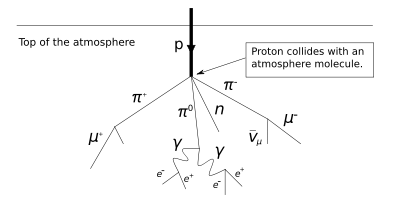
\includegraphics[scale=.5]{figs/cosmicray.jpg}
%\caption{Cosmic Ray Shower}
%\label{fig:cosmicray}
%\end{figure}

In general, these neutrinos have energies from 1 GeV to 100s of GeV and the ratio of $\nu_{\mu}$'s to $\nu_{e}$'s equals to 2 (see equation \ref{eq:ratio})
\begin{equation}
\label{eq:ratio}
R = \frac{(\nu_{\mu} + \overline{\nu_{\mu}})}{(\nu_{e} + \overline{\nu_{e}})}
\end{equation} 


There have been two types of detectors used to study atmospheric neutrinos: Water Cherenkov detectors and tracking calorimeters. Atmospheric detector experiments measure the ratio of $\nu_{\mu}$ to $\nu_{e}$. They also measure the zenith angle distribution of the neutrinos. These experiments report a double ratio (shown in equation \ref{eq:doubleratio}). This double ratio is the ratio measured in the detector to the ratio that's expected which is 2. If the double ratio equals to 1, the data agrees with the prediction. Various measurements from multiple experiments are shown in figure \ref{fig:ratiotable}. Except for Frejus, all R measurements are less than 1. This discrepancy between the predicted R and the measured R became known as the Atmospheric Neutrino Anomaly \cite{superk}.
\begin{equation}
\label{eq:doubleratio}
R = \frac{(N_{\mu}/N_{e})_{DATA}}{(N_{\mu}/N_{e})_{SIM}}
\end{equation}

\begin{table}[htp!]
\centering
\caption{Measurements of the double ratio for various atmospheric neutrino experiments}
\label{fig:ratiotable}
\resizebox{0.7\textwidth}{!}{\begin{tabular}{c c c}
\hline
Experiment & Type of experiment & R\\
\hline
Super-Kamiokande & Water Cherenkov & 0.675 $\pm$ 0.085\\ 
Soudan2 & Iron Tracking Calorimeter & 0.69 $\pm$ 0.13\\
IMB & Water Cherenkov & 0.54 $\pm$ 0.12\\
Kamiokande & Water Cherenkov & 0.60 $\pm$ 0.07\\
Frejus & Iron Tracking Calorimeter & 1.0 $\pm$ 0.15\\
\hline
\end{tabular}}
\end{table}

Kamiokande-II has the capability of measuring the direction of the incoming neutrinos. The expectation of atmospheric neutrino detection is that the flux will be isotropic due to the fact that atmospheric neutrinos can reach the detector from all directions. Kamiokande-II noticed that muon-like data did not agree well with this expectation. At low energies approximately half of the $\nu_{\mu}$ are missing over the full range of zenith angles. At high energies the number of $\nu_{\mu}$ coming down from above the detector seems to agree with expectation, but half of the same $\nu_{\mu}$ coming up from below the detector are missing. This anomaly can be easily explained by neutrino flavor oscillations. Due to the fact that the neutrino travels less distance coming straight down into the detector (about 15 km) than coming up from the bottom of the detector(13000 km) changes the probability of oscillation. The probability of oscillation for the muon neutrinos coming down into the detector is roughly zero, whereas for neutrinos coming up, the oscillation probability is $\text{sin}^2(2\theta$). Both the solar and atmospheric neutrino problems can be explained by neutrino oscillation so it's fitting to derive this phenomenon mathematically. In the next two sections, two flavor and three flavor neutrino oscillation derivations will be explained. 


\section{Neutrino Oscillations}\label{section:oscillations}
Neutrino oscillation was first predicted by Bruno Pontecorvo \cite{pontecorvo}. It describes the phenomenon of a neutrino created with a specific lepton flavor (electron, muon or tau) that is later measured to have a different flavor. Neutrino oscillation is important theoretically and experimentally due to the fact that this observation implies that the neutrino has a non-zero mass, which is not part of the original Standard Model of particle physics. 

\subsection{Two Flavor Neutrino Oscillation Formulation}
The flavor eigenstates can oscillate between each other because they are composed of an add mixture of mass eigenstates($\nu_{1}$,$\nu_{2}$). Figure \ref{fig:mixing} shows the mass and flavor eigenstates rotated by an angle $\theta$ which is the mixing angle. 

In matrix form the wave-functions are:

\begin{equation}
\begin{pmatrix}
\nu_{\mu} \\
\nu_{e}
\end{pmatrix} 
 = \begin{pmatrix}
cos\theta & sin\theta \\
-sin\theta & cos\theta 
\end{pmatrix}*
\begin{pmatrix}
\nu_{1} \\
\nu_{2} 
\end{pmatrix}
\end{equation}

\begin{figure}[htp]
\centering
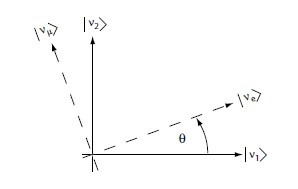
\includegraphics[scale=.8]{figs/mixingangle.jpg}
\caption{The flavor eigenstates are rotated by an angle $\theta$ with respect to the mass eigenstates}
\label{fig:mixing}
\end{figure}
Applying the time evolution operator to $\nu_{\mu}$:
\begin{equation}
\centering
\label{eq:timeevol}
|\nu_{\mu}(t)> = -sin\theta|\nu_{1}>e^{-i\frac{E_{1}t}{\hbar}} + cos\theta|\nu_{2}>e^{-i\frac{E_{2}t}{\hbar}}
\end{equation}
where $E_{1} = \sqrt{p^2 c^2 + m^2_{1} c^4}$ and $E_{2} = \sqrt{p^2 c^2 + m^2_{2} c^4}$ and $p_{1}=p_{2}$. For the time being, let us assume $\hbar=c=1$. 
With this assumption:
$E_{1}=\sqrt{p^2+m^2_{1}}$ and $E_{2} = \sqrt{p^2 + m^2_{2}}$.
The next modifications is to assume neutrinos are relativistic:
\begin{equation}
\centering
\label{eq:gamma}
\gamma = \frac{E}{m^2_{o} c^2} = \frac{\sqrt{p^2 c^2 + m^2_{o} c^4}}{m_{o} c^2} \gg 1
\end{equation}
because of this,
\begin{equation}
\centering
p \gg m_{o}
\end{equation}
\begin{equation}
\centering
E = \sqrt{p^2 + m^2_{o}}=p\sqrt{1+m^2_{o}/p^2}\simeq p + \frac{1}{2}\frac{m^2_{o}}{p}
\end{equation}
where the binomial expansion is used. Now $E_{1}$ and $E_{2}$ can be written as:
\begin{equation}
\centering
E_{1} \simeq p + \frac{1}{2}\frac{m^2_{1}}{p} \mbox{    and    }  E_{2} \simeq p + \frac{1}{2}\frac{m^2_{2}}{p}
\end{equation} 
Now applying all these assumptions back into equation \ref{eq:timeevol} gives us:
\begin{equation}
\centering
|\nu_{\mu}(t)> = -sin\theta|\nu_{1}>e^{-i\left( p+\frac{1}{2}\frac{m^2_{1}}{p}\right)t} + cos\theta|\nu_{2}>e^{-i\left(p+\frac{1}{2}\frac{m^2_{2}}{p}\right)t}
\end{equation}
\begin{equation}
\centering
|\nu_{\mu}(t)> = e^{-i \left( p+\frac{1}{2}\frac{m^2_{1}-m^2_{2}}{p} \right) t} \left( -sin\theta|\nu_{1}> + cos\theta|\nu_{2}> \right)
\end{equation}
Substituting $\Delta m^2 = m^2_{1}-m^2_{2}$ and $t = \frac{x}{c} =x$ and $e^{-iz}= e^{-i \left( p+\frac{1}{2}\frac{m^2_{1}}{p} \right) t}$ gives us:
 \begin{equation}
 \centering
 |\nu_{\mu}(t)> = e^{-iz} \left( -sin\theta|\nu_{1}> + cos\theta|\nu_{2}>e^{+ix \left(\frac{1}{2}\frac{\Delta m^2}{p}\right)}\right)
 \end{equation}
Finding the Probability for a $\nu_{\mu} \rightarrow \nu_{e}$:
\begin{equation}
\centering
P(\nu_{\mu} \rightarrow \nu_{e}) = |<\nu_{e}|\nu_{\mu}(t)>|^2
\end{equation}
Remembering that $<\nu_{i}|\nu_{j}>=\delta_{ij}$
\begin{equation}
\centering
<\nu_{e}|\nu_{\mu}(t)> = e^{-iz}\left(-sin\theta cos\theta + sin\theta cos\theta e^{\frac{i \Delta m^2 x}{p}}\right)
\end{equation}
Taking the absolute value squared gives us:
\begin{equation}
\centering
P(\nu_{\mu} \rightarrow \nu_{e}) = |<\nu_{e}|\nu_{\mu}(t)>|^2 = e^{+iz}e^{-iz}sin^{2}\theta cos^{2}\theta\left( -1 + e^{\frac{i \Delta m^2 x}{p}}\right)\left(-1 + e^{\frac{i \Delta m^2 x}{p}}\right)
\end{equation}
Since the neutrino is relativistic we can set $p= E_{\nu}$ and change $x=L$. Also recognizing the trigonometric relation $(1 - cos2\theta)/2 = sin^{2}\theta$ the above equation becomes:
\begin{equation}
\centering
P(\nu_{\mu} \rightarrow \nu_{e}) = sin^{2}2\theta sin^2\left(\frac{\Delta m^2 L}{4 E_{\nu}}\right)
\end{equation}
All that's left to do now is re-introduce $\hbar$ and $c$ doing this we get:
 \begin{equation}
 \centering
 P_{\nu_{\mu} \rightarrow \nu_{e}} (L,E) = sin^{2}2\theta sin^2\left(1.27 \Delta m^2 \frac{L}{E_{\nu}}\right)
 \end{equation}
 
This equations has three important variables. 
 \begin{itemize}
 \item The angle $\theta$: This angle, as mentioned before, is called the mixing angle. It defines the difference between the flavor and the mass eigenstates. When $\theta = 0$ the mass and flavor eigenstates are identical and no oscillations occur. 
 \item The mass squared difference, $\Delta m^2$: Again $\Delta m^2 = m^2_{1}-m^2_{2}$. The reason this is an important variable is because it implies that for neutrinos to oscillate, neutrinos must have mass. Furthermore, the mass squared difference also tells us that the neutrino mass eigenstates must be different. 
 \item L/E: This is the variable that is of most interest to experimental physicists due to the fact that it is the variable that we set. L is the distance between the source and detector and E is the energy of the neutrino. For a given $\Delta m^2$, the probability of oscillation changes with respect to L/E. 
 \end{itemize}

\subsection{Three Flavor Neutrino Oscillation Formulation}
Seeing the quantum mechanics involved in deriving the probability of a two flavor neutrino oscillation, it is now possible to formulate the three flavor neutrino oscillation. The three flavor neutrino oscillation formulation begins  similarly to the two flavor, but there is the Pontecorvo-Maki-Nakagawa-Sakata matrix (PMNS) instead of the 2X2 matrix in the previous section. The PMNS matrix is show below:
\begin{equation}
\centering
\begin{pmatrix}
c_{12}c_{13} & s_{12}c_{13} & s_{13}e^{-i \delta} \\
-s_{12}c_{23} - c_{12}s_{23}s_{13}e^{i \delta} & c_{12}c_{23} -s_{12}s_{23}s_{13}e^{i \delta} & s_{23}c_{13}\\
s_{12}s_{23} - c_{12}c_{23}s_{13}e^{i \delta} & -c_{12}s_{23} - s_{12}c_{23}s_{13}e^{i \delta} & c_{23}c_{13}
\end{pmatrix} *
\begin{pmatrix}
e^{i \alpha_{1}/2} & 0 & 0\\
0 & e^{i \alpha_{2}/2} & 0\\
0 & 0 &1
\end{pmatrix}
\end{equation} 
where $c_{ij}=cos\theta_{ij}$ and $s_{ij}=sin\theta_{ij}$
Following the same steps as before we get:
\begin{equation}
\centering
P_{\alpha \rightarrow \beta}= \delta_{\alpha \beta} - 4 \Sigma Re(U^{*}_{\alpha i} U_{\beta i} U{\alpha j} U^{*}_{\beta j})sin^{2}\left(\frac{\Delta m^{2}_{ij} L}{4E}\right) 2 \Sigma Im(U^{*}_{\alpha i} U_{\beta i} U{\alpha j} U^{*}_{\beta j})sin\left(\frac{\Delta m^{2}_{ij} L}{2E}\right)
\end{equation}

The main things to notice here are $\delta_{ij}$ which is the CP violating term and has not been measured yet, and $\theta_{13}$ which has just been measured. CP violation is a violation of the postulated CP-symmetry. CP-symmetry states that the laws of physics should be the same if a particle were to be exchanged with its antiparticle and then if the left hand side of a decay were switched with the right hand side. Table \ref{table:measurements} shows the current knowledge of the values of all the fundamental parameters for neutrino oscillations \cite{pdg}. 
\begin{table}[htp!]
\centering
\caption{Current knowledge of neutrino oscillation parameters \cite{pdg}}
\label{table:measurements}
\resizebox{0.5\textwidth}{!}{\begin{tabular}{c c}
\hline
Parameter & Value\\
\hline
$\theta_{12}$ & $33.9 \pm 1.0^\circ$\\
$\theta_{23}$ & $39^\circ < \theta_{23} < 51^\circ$\\
$\theta_{13}$ & $9.1 \pm 0.6^\circ$\\
$\Delta m^2_{21}$ & $(7.50 \pm 0.20)*10^{-5} \text{eV}^2$\\
$|\Delta m^2_{32}|$ & $(2.32^{+0.12}_{-0.08})*10^{-3} \text{eV}^2$\\
$\delta_{cp}$ & unknown\\
\end{tabular}}
\end{table}

\section{Neutrino Interactions}
As stated previously, neutrinos interact via the weak force, because of this, we do not directly see the path of the neutrino through a detector. It is important to understand neutrino interactions, and hence cross-sections before precision measurements of neutrino oscillations can be determined. 
\subsection{Weak Interactions}
The weak force has two forms, charged-current (CC) interactions which are mediated by the $W^{\pm}$ boson, and neutral-current (NC) which are mediated by the $Z^0$ boson. These bosons are very heavy \cite{griffiths}. Their masses have been measured to be \ref{eq:masses}.
\begin{equation}
M_w = 82 \pm 2 GeV/c^2,	M_z = 92 \pm 2 Gev/c^2
\label{eq:masses}
\end{equation}
The currents for CC and NC interactions are shown in \ref{eq:currents}
\begin{equation}
j^{\pm}_{\mu} = \overline{u}\frac{-ig_{W}}{2\sqrt(2)}(\gamma^{\mu}-\gamma^{\mu}\gamma^{5})u
j^{0}_{\mu} = \overline{u}\frac{-ig_{z}}{2}(g_v\gamma^{\mu}-g_A\gamma^{\mu}\gamma^{5})u
\label{eq:currents}
\end{equation}
where:
\begin{conditions}
u and \overline{u} & Dirac spinors\\
\gamma^{\mu} & four Dirac gamma matrices\\ 
\gamma^5,	g_W and g_Z & coupling strengths\\
\end{conditions}

Rewriting the current equation to \ref{eq:chiralcurrent} shows the weak force's chiral nature. Chirality is a property of the particle spinors. It is Lorentz invariant but not constant in time. Chiral Eigenstates are either left or right-handed and are defined by the chirality operator $\gamma^5$ with eigenvalues -1 for left-handed or +1 for right-handed. Particle spinors are generally composed of both chiral components. 
\begin{equation}
j^{\pm}_{\mu} = \overline{u}\frac{-ig_{W}}{2\sqrt(2)}\gamma^{\mu}(1\pm\gamma^{5})u
\label{eq:chiralcurrent}
\end{equation}

Expanding the negative \ref{eq:chiralcurrent} using the chiral projection operators we get \ref{eq:chiralexpanded}. Written this way, it can be seen that CC weak interactions are vector currents that interact only with the left-handed chiral component of a particle, or right-handed chiral component of an anti-particle. 
\begin{equation}
j^{-}_{\mu} = \frac{-ig_{W}}{2\sqrt(2)}\overline{u}(1+\gamma^{5})\gamma^{\mu}(1-\gamma^{5})u = \frac{-ig_{W}}{2\sqrt(2)}\overline{u_L}\gamma^{\mu}u_L
\label{eq:chiralexpanded}
\end{equation}
The same conclusion arises with the NC weak interactions. Due to neutrinos only being created via the weak force, neutrinos then are always created in the left-handed chiral eigenstate. Even though neutrinos are only created in a left-handed chiral state, they will gradually evolve a right-handed chiral component. 

\subsection{Neutrino-Nucleon Interactions}
The four momentum transferred between the neutrino/lepton system and the target is denoted as q. The square of this transfer, $Q^2$ is Lorentz invariant. Small $Q^2$ are dominated by elastic interactions and are when the struck nucleon recoils from the interaction without breaking. In the CC case, there is also a change of charge. Because of the transfer of mass to the final state lepton, CC interactions are more correctly called quasi-elastic (QE). For the NC case, all neutrinos and anti-neutrinos can scatter off both neutrons and protons and is referred to as NC-elastic scattering. At high $Q^2$, it becomes unlikely for the nucleon to remain intact, therefore the CCQE cross-section becomes negligible. 

CCQE interactions allow for the kinematics to be completely reconstructed because of the two-body interaction and therefore the initial neutrino energy can be determined. As discussed in section \ref{section:oscillations}, accurately determining the initial neutrino energy is critical for measuring the oscillation parameters. 

For inelastic interactions, low $Q^2$ are dominated by resonance (RES) productions. A resonant interaction is when a nucleon is excited into a baryonic resonance before decaying. Understanding CCRES is important for neutrino oscillation experiments searching for $\nu_e$ because a CCRES interaction producing a $\pi^0\rightarrow2\gamma$ can mimic an electron. 

At high $Q^2$, the inelastic interactions are dominated by deep inelastic scattering (DIS). DIS is when the neutrino scatters off of a quark inside the nucleon, breaking the original nucleon. At energies below 1 GeV, CCQE interactions dominate, however there is a rapidly varying transition region where there are fractions of each channel. Figure \ref{fig:xsec_zellar} \cite{zellar} shows the neutrino cross section as a function of energy for the different CC interactions. 

At low neutrino energies, a neutrino can undergo NC coherent (COH) scattering. Coherent scattering occurs when the nucleus recoils as a whole and is left in the same state as when the neutrino arrived. NCCOH scattering results in a slight recoil of the struck nucleus. At higher neutrino energies, both CC and NC COH scattering is possible which then results in an additional final state particle suck as a $\pi$, $\rho$ or K meson. The four-momentum transfer to the nucleus needs to be kept small in COH scattering and this strongly constrains the kinematics. The final state lepton and particles created are created at small scattering angles relative to the incoming neutrino. This constraint also results in a small COH cross-section. 

Although the COH cross-sections are low, coherent pion production is also important to understand for oscillation experiments searching for $\nu_e$ due to the two photons that decay from an NCCOH $\pi^0$ production mimicking an electron, similar to a RES $\pi^0$. 
\begin{figure}[htp]
\centering
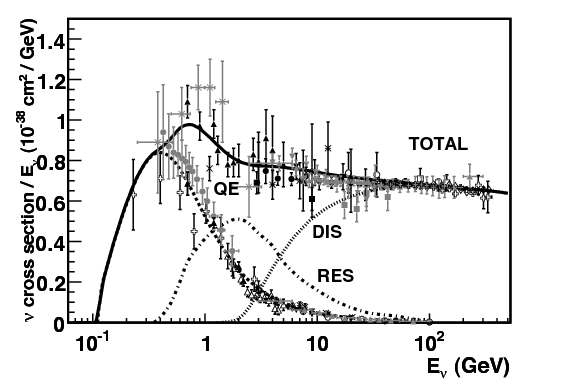
\includegraphics[scale=.55]{figs/cc_inclusive_nu.png}
\captionof{figure}{Total neutrino per nucleon CC cross sections divided by neutrino energy and plotted as a function of energy. Predictions for the processes are by the NUANCE generator. \cite{zellar}}
\label{fig:xsec_zellar}
\end{figure}


%\subsection{Reactor Oscillation}
%Many experiments have searched for oscillation of electron anti-neutrinos produced at nuclear reactors. Such oscillations give the value of the parameter $\theta_{13}$. The KamLAND experiment, started in 2002, has made a high precision observation of reactor neutrino oscillation. Neutrinos produced in nuclear reactors have energies similar to solar neutrinos, a few MeV. The baselines of these experiments have ranged from tens of meters to over 100 km. On 8 March 2012, the Daya Bay team announced a 5.2$\sigma$ discovery that $\theta_{13}\neq 0$. %Two other experiments are currently measuring reactor neutrino oscillation (at the same baseline of a few kilometers) and may eventually confirm the Daya Bay results: Double Chooz and RENO.


%\section{Beam Oscillation}
%Neutrino beams produced at a particle accelerator offer the greatest control over the neutrinos being studied. Many experiments have taken place which study the same neutrino oscillations which take place in atmospheric neutrino oscillation, using neutrinos with a few GeV of energy and several hundred km baselines. The MINOS experiment recently announced that it observes consistency with the results of the K2K and Super-K experiments.
%The controversial observation of beam neutrino oscillation at the LSND experiment in 2006 was tested by MiniBooNE. Results from MiniBooNE appeared in Spring 2007, and appeared to contradict the findings of the LSND experiment. Results from the HARP-CDP group also put the LSND result into doubt.
%On 31 May 2010, the INFN and CERN announced having observed a tau particle in a muon neutrino beam in the OPERA detector located at Gran Sasso, 730 km away from the neutrino source in Geneva.
%The currently-running T2K experiment uses a neutrino beam directed through 295 km of earth, and will measure the parameter θ13. The experiment uses the Super-K detector. NOνA is a similar effort. This detector will use the same beam as MINOS and will have a baseline of 810 km.


%\section{Unanswered questions about Neutrinos }
%There are many questions that haven't been answered by previous experiments. Many of them I have touched upon in previous sections, but here is a formal list of questions left unanswered. 
%\begin{itemize}
%\item What is the sign of $\Delta m^{2}_{23}$?
%\item Are there more than three active neutrinos? (LSND experiment)
%\item Are the neutrinos and antineutrinos identical?
%\item Is there a CP violating term that needs to addressed. 
%\item Will $\delta_{cp}$ explain matter-antimatter asymmetry?  
%\item Why is the PMNS matrix so different in form to the CKM matrix( quark mixing matrix)
%\end{itemize}


%\section{Final Thoughts}
%Although there is much about neutrinos that we don't know, we have made much progress in trying to understand these elusive particles. We now know that neutrinos aren't massless and because of this knowledge we now know that neutrinos oscillate between flavor and mass eigenstates. We have also just recently discovered that $\theta_{13}$ is non-zero and this knowledge will lead to experiments and data analysis to find $\delta_{cp}$.
%\clearpage

%More introduction

  \chapter{The MicroBooNE Experiment}
The purpose of this chapter is to discuss and understand the details of the MicroBooNE detector. A thorough understanding of MicroBooNE and the technology behind liquid argon time projection chambers is important for understanding results as well as understanding how images were made for use in deep learning efforts that will be outlined in later chapters.   

\section{Introduction}
The experimental study of neutrinos is central to FermiLab's scientific program and offers the possibility for exciting discoveries that could reshape our understanding of the universe. Liquid Argon Time Projection Chambers (LArTPCs) are an exciting detector technology that provide excellent imaging and particle identification, and are now being used to study neutrinos. In these detectors, liquid argon (LAr) is the medium used to detect neutrinos. When a neutrino interacts with an argon atom, the charged particles that are produced ionize the LAr as they travel away from the interaction. By placing a uniform electric field throughout the LAr, the ionization is made to drift towards a set of anode planes, which consist of wires spaced very closely together collecting the ionized charge, which is subsequently read out by electronics connected to the anode wires. The collected ionization creates a spatial image of what happened in the detector on each anode plane. The $\nu-Ar$ interaction also produces scintillation light which is collected by photomultiplier tubes (PMTs) which allows the exact time of the neutrino interaction to be determined. The drift time of the ionization relative to the time of the original signal allows the signal to be projected back along the drift coordinate, hence the name LArTPC. Having very small distances between each wire within an anode plane allows for very fine granularity and detail to be captured, and having multiple wire planes at different angles coupled with exact timing of neutrino interaction, provides independent two-dimensional views that can be combined into a three dimensional picture of the interaction. Once the charge signal is created on the anode planes, software analysis packages identify particles in the detector by using deposited energy on the wires along their track length. 

MicroBooNE (Micro Booster Neutrino Experiment) is a ~89 T active volume (180 T total mass) LArTPC which is then inserted into a cylindrical crysotat on axis of the Booster Neutrino Beam (BNB) stationed at Fermilab in Batavia, Illinois. The main components of MicroBooNE will be detailed in the upcoming sections. MicroBooNE is also an R\&D detector that can be scaled up to a significanlty larger size, such as Deep Underground Neutrino Experiment (DUNE) which is roughly 40 kT compared to MicroBooNE at 180T \cite{dune}. Understanding LArTPC technology and detector physics is necessary to build a LArTPC the size of DUNE, and MicroBooNE has made many advances in developing this technology\cite{noisechar} \cite{michel}. 
\section{Time Projection Chamber}
MicroBooNE's Time Projection Chamber (TPC) is 10.3 m long (beamline direction), 2.3 m high and 2.5 m wide (which corresponds to the drift distance). The TPC is shown in figure \ref{fig:tpc}. MicroBooNE is the largest LArTPC currently running in the world\cite{microboone}. This LArTPC has 3 wire planes: 1 plane that collects the ionization in the wires and is $0^{\circ}$ to the virtical with 3456 wires spaced 3 mm apart, and 2 planes where the ionization drifts passed and induces a signal at $+/- 60^{\}circ}$ to the vertical each with 2400 wires also spaced 3 mm apart. Each plane has a spacing also of 3 mm from eachother. The wires are then connected to detector specific circuit boards (ASICS) that are submered and operate inside liquid argon. The first two planes are the induction planes and the last is the collection. The electric field of the TPC is created using 64 stainless steel tubes shaped into rectangules around the TPC and held in place by G10 to form a field cage. The cathode is charged at a high voltage of -70 kV and this voltage is stepped down across the field cage tubes using a voltage divider chain with an equivalent resitance of 240 M\ohm between the tubes. The field cage tubes are separated by 4 cm from center to center. 
\section{Light Collection System}
The light collection system is a crucial part for 3D reconstruction of particle interactions in the LArTPC. It is possible to reconstruct interactions using just the wire signals, but without the initial timing (t0) of an event, it is impossible to position the event along the drift direction. When a particle interaction occurs, the scintillation light created propogates within nanoseconds to the light collection system compared to the milliseconds it takes the ionized electrons from the interaction to reach the anode wire planes. Therefore we can precisely know where along the drift direction the particle interaction first took place. The scintillation light is also localized, so combining the PMT information with the wire plane information allows for cosmic background rejection happening outside the beam timing window.  

The light collection system is made up of 32 Hammamatsu R5912-02mod cryogenic PMTs with a diameter of 8-inches. The PMTs are are located behind the 3 wire anode planes and provides 0.85\% photocathode coverage. Each PMT has an acrylic plate mounted in front of it that is coated with a wave-length shifting material called TPB. The acrylic plates take in the scintillation light, at 128 nm, and re-emits it visible wavelengths visible to the PMTs, with a peak at 425 nm. 
\section{Electronics System} 
More MicroBooNE stuff.

  %\chapter{The Booster Neutrino Beam}
Chapter about the beam
\clearpage
\dots

  \chapter{Neutrino Identification: Finding MicroBooNE's first Neutrinos} \label{ch:neutrinoID}
The goal of the Neutrino Identification analysis was to positively identify BNB neutrino interactions in the MicroBooNE detector collected during the first days of running. Neutrino event candidates were identified in part by using a cut on detected flash of scintillation light during the 1.6 $\micro s$ beam-spill length of the BNB as well as identifying reconstructed object from the TPC that are neutrino like. After this selection, 2D and 3D event displays were used for verification of the selection performance. This selection was targeted to reduce the ratio of neutrino events to cosmic-only events from the initial 1 neutrino to 675 cosmics to a ratio of 1 to 0.5 or better which is equivalent to a background reduction by a factor of 1000 or more. These selected events were used for MicroBooNE's first public displays of neutrino interactions. A clearly visible neutrino interaction with an identifiable vertex and at least 2 tracks originating from the vertex was what the analysis focused on. This analysis wasn't optimized for high purity or efficiency, but rather for very distinguishable neutrino interactions that could be shared with the public. The description of this analysis below as well as all figures come from MicroBooNE-Note-1002-Pub \cite{neutrinoid} and the corresponding internal note.
\section{Flash Finding}\label{sec:flashfinding}
Flash finding is the first step used in finding neutrino interactions. This section will detail how optical information is reconstructed as well as how analysis scripts and event filters were used.
\subsection{Flash Reconstruction}
\begin{figure}[htp!]
\centering
	\begin{subfigure}[b]{.6\textwidth}
	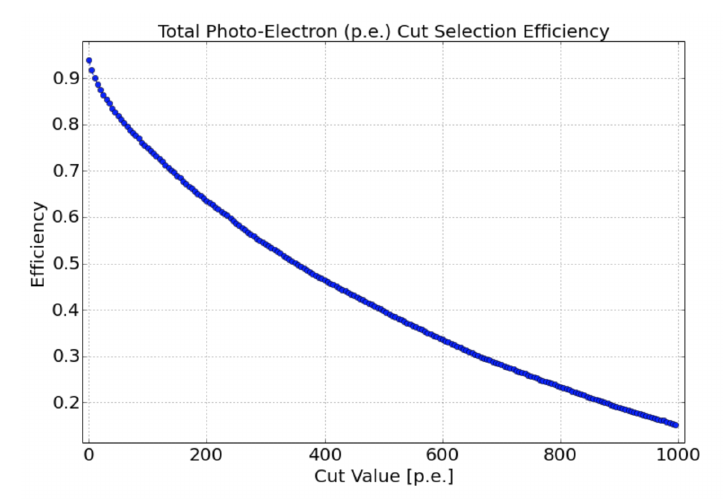
\includegraphics[width=\textwidth]{figs/totalpecut.png}
	\end{subfigure}
	\quad
	\begin{subfigure}[b]{.6\textwidth}
	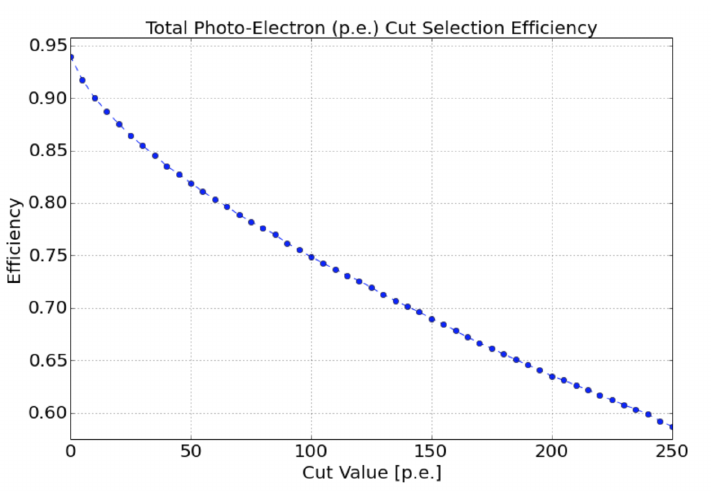
\includegraphics[width=\textwidth]{figs/totalpe_zoomed.png}
	\end{subfigure}
	\quad
\caption{Top: Efficiency for selecting beam events as a function of minimum total PE cut. Bottom: Zoomed into interesting region.}
\label{fig:PE}
\end{figure}
A flash is described as a collection of light seen at the same time within the detector. They are reconstructed by identifying coincident signal from the PMTs above a specific photoelectron (PE) threshold. These signals are called optical hits. Optical hits from all the PMTs are then accumulated into 1 $\micro s$ bins of time. If a specific bin is above a set PE threshold, then the optical hits that overlap in time are the labeled as the hits from the flash. All flash reconstructed properties like average time and x/y positions are then found via the flash labeled optical hits. The total size of the flash is found by summing up the total number of photoelectrons from all PMTs. Neutrino interactions and cosmic muons will have a larger flash size compared to noise and other low-energy backgrounds, therefore a total PE cut is used to reject these backgrounds. A total PE cut of 50 PE was deemed sufficient for this analysis. Figure \ref{fig:PE} show the total PE versus the selection efficiency of neutrino beam events. 


\subsection{Beam Timing}
\begin{figure}[htp!]
\centering
	\begin{subfigure}[b]{.6\textwidth}
	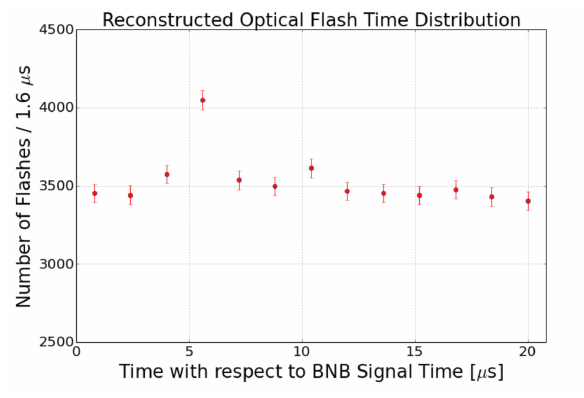
\includegraphics[width=\textwidth]{figs/flashrate_sim.png}
	\caption{Predicted distribution of flash times with respect to trigger time for 1 day of data taking at nominal rate and intensity}
	\label{fig:pe_sim}
	\end{subfigure}
	\quad
	\begin{subfigure}[b]{.6\textwidth}
	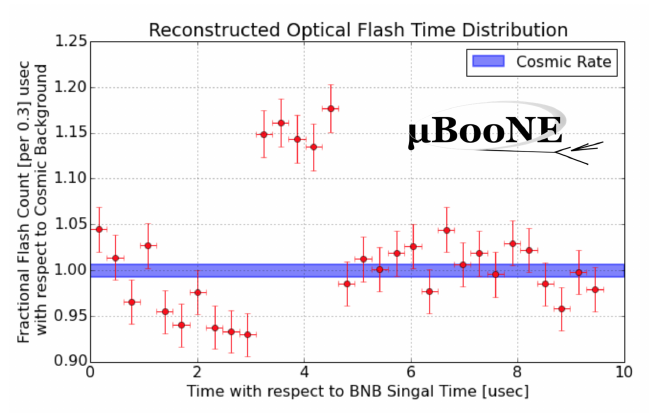
\includegraphics[width=\textwidth]{figs/flashrate.png}
	\caption{Measured distribution of flash times with a 50 PE threshold cut, with respect to trigger time. Shown as a ratio to the expected cosmic rate from off-beam data. A clear excess from neutrinos is visible between 3- 5 $\micro s$ after the trigger time. }
	\label{fig:pe_data}
	\end{subfigure}
	\quad
\label{fig:petime}
\end{figure}
It is necessary to get the specific time from flashes if one uses flashes to filter out background from neutrino interactions coincident with the neutrino beam spill period. Before a filter can be applied, an understanding of the timing of the trigger and PMT readout with respect to the arrival of neutrinos from the BNB is necessary. To do this, a 1.6 $\micro s$ window near the expected beamtime was created and verified by finding that the number of flashes was significantly above the cosmic-ray background flashes. Beam data during the first week of running, October 16th 2016 through October 22nd 2016, were used for a timing measurement. The total POT used corresponds to roughly 24 hours of data taking at nominal intensity ($4 X 10^{12} ppp$) and a 5 Hz repetition rate. Figure \ref{fig:pe_sim} shows the size of the expected neutrino signal in time using MC predictions and figure \ref{fig:pe_data} shows the neutrino signal in data. The intensity in data is lower, however a significant excess above data can still be seen.

\subsection{Event Rates}
Applying a 50 PE threshold cut inside a 1.6 $\micro s$ window reduces the cosmic-ray passing rate to 0.8\%. With a 5 Hz beam rate, this corresponds to 135 cosmics passing per hour. The neutrino passing rate for this filter is about 22 events per hour. To further increase the neutrino to cosmic ratio, TPC topology cuts were implemented and will be discussed in the following section.
\section{TPC Topology Selection}  
In order to further reduce the background of cosmic events, two independent selection streams using TPC wire data reconstruction were implemented. The first using 2D reconstructed clusters, and the second using 3D reconstructed tracks. Both streams look for neutrino interactions in the active TPC volume which are identifiable by two or more tracks originating from the same vertex.

Both 2D and 3D channels were optimized using MC simulation which used a 128 kV cathode voltage. Passing rates were calculated using a 0.8\% efficiency factor for cosmic events passing to simulate the flash finding described in section \ref{sec:flashfinding}. This efficiency factor was an overestimation and was just used to get a general feel of what signal and background rates we would actually see in data. 
\subsection{Cosmic Tagging}
The first step in TPC selection was based on the geometry of cosmic tracks in an event. The cosmic ray muon geometry tagger runs on 3D tracks and assigns a score to each reconstructed track on the likeliness of the track originating from a cosmic. The cosmic scores are detailed below:
\begin{itemize}
\item 1: The track is tagged as entering or entering the TPC
\item 0.95: The track is a delta ray associated with a tagged track
\item 0.5: The track is either entering or exiting, but not both
\item 0.4: The track is entering or exiting through the Z boundary
\item 0: The track isn't tagged
\end{itemize}
Clusters are assigned either a 0 or 1, 1 being a cosmic. In simulation, 90\% of cosmics are tagged as cosmics. These tracks are no longer considered when looking for a neutrino topology. Requiring that the tracks be contained in turn affects the neutrino efficiency by 20\%. The algorithm checks that each track is contained within a boundary region of 10 cm from all sides of the TPC. This boundary region was optimized via handscanning of experimental data.

As can be expected, cosmic tagging is more efficient in the 3D channel (tracks) than the 2D channel (clusters) because the reconstructed tracks can use the full 3D position information of the entering and exiting points while the 2D channel mainly use the reconstructed x position of the cluster which is associated to timing. 

Cosmic tagging uses timing information to reject tracks and clusters that are outside of drift window. The drift window for 128 kV is 1.6 $\micro s$ while for 70 kV, the actual voltage MicroBooNE is running at, is 2.3 $\micro s$. Due to this variation between simulation and data, we expect to see $2.3/1.6 = 1.44$ times more cosmic induced tracks or clusters in the drift window. 
\subsection{2D Cluster Selection}
After looking at experimental cosmics data, 2D clustering performs well, while 3D track reconstruction is affected by more variations in simulation, for example noise filters. This was the motivation for having a selection only on 2D clusters in the collection (Y) plane. As stated previously, the goal of this analysis was to find identifiable neutrino interactions for use in public event displays, in future analyses, the 3D track reconstruction has been modified to further increase the tracking efficiency and has more information than just the clusters. For this analysis, however, 2D cluster information was sufficient enough for neutrino selection. 
\subsubsection{Primary Cuts}
The first cuts were used to select which clusters to consider. First the clusters must have at least ten hits on the collection plane and have a cosmic tagging score < 0.4. Only events that have at least two clusters that satisfy these primary cuts continue on.

After the initial cosmic tagging is applied, the following cuts are used to furture separate identifiable neutrinos for background cosmics. 

The next cut was to remove long, vertical clusters. This was applied after seeing that most cosmic induced clusters passing were long with high angles, while neutrino induced clusters were mainly forward going. We required a good cluster to either have a projected start angle less than 30 degrees from the z axis or be less than 200 wires long. The length cut was added to make sure we don't cut any short high angle clusters that can correspond with a proton, or other highly ionizing particle associated with a long muon cluster. The 200 wire cut roughly equates to 0.6 m in the z direction, with a 3 mm wire pitch. Also, the projected angle is defined by tan $\alpha$ = $\Delta T / \Delta W$ where T is the time ticks and W is the wires. 

The last cut requires the clusters to be either 30 time ticks or 30 wires. This cut was applied to reduce small delta rays associated with a cosmic without removing proton clusters associated with a long muon cluster, which saves ideal neutrino events that have both a long minimum ionizing muon like cluster and a short highly ionizing proton like cluster.

\subsubsection{Secondary Cuts}
The secondary cuts look to match long, low-angle clusters with short, high-charge clusters. Only clusters that have passed previous cuts are used. First clusters with length greater than 100 wires are chosen, which is approximately 0.3 m in the z direction. Then we search for any cluster that is within approximately 3 cm ( 10 wires and 30 time ticks) away from the low-z end of the long cluster. This cluster must also be shorter than the first. In our reconstruction, the start and end point of a cluster can be swapped so both ends of the short cluster are compared to the long cluster. 

Now that there is a vertex match, cuts based on charge and projected opening angle are implemented. We require the short cluster to have a higher start charge than the long cluster or the long cluster be longer than 500 wires. Start charge is defined as the charge on the first wire in ADC counts. The projected opening angle must also be between 11 and 90 degrees. This last cut is intended to remove clusters that are entirely overlapping or are part of the same long track. 
\begin{table}
\begin{center}
\begin{tabular}{c c c c}
\hline
Cluster set & No Cuts & Primary Cuts & Secondary Cuts \\
\hline
Neutrinos only & 570 & 303 & 32 \\
Cosmics only ( no flash) & 308,016 & 291,879 & 602 \\
Cosmics only (w/ flash) & 2464 & 2335 & 5 \\
\hline
Neutrinos/Cosmics & 0.23 & 0.13 & 6.4 \\
\end{tabular}
\caption{Passing rates for 2D cluster cuts for neutrino on MC set and a cosmic only MC set. First column shows event rates with no cuts applied to both sets. Columns two and three show event rates after primary and secondary cuts are applied. Line three shows the second line scaled with the flash finding factor of 0.008. All events are normalized to per day assuming we are running at 5 Hz.}
\label{table:eventrate}
\end{center}
\end{table}
The resulting neutrino/cosmic event rate per day is shown in table \ref{table:eventrate}. Figures \ref{fig:2dprimarycut} and \ref{fig:2dsecondarycuts} shows the percentages of clusters that pass each primary and secondary cuts.     

\begin{figure}[htp!]
\centering
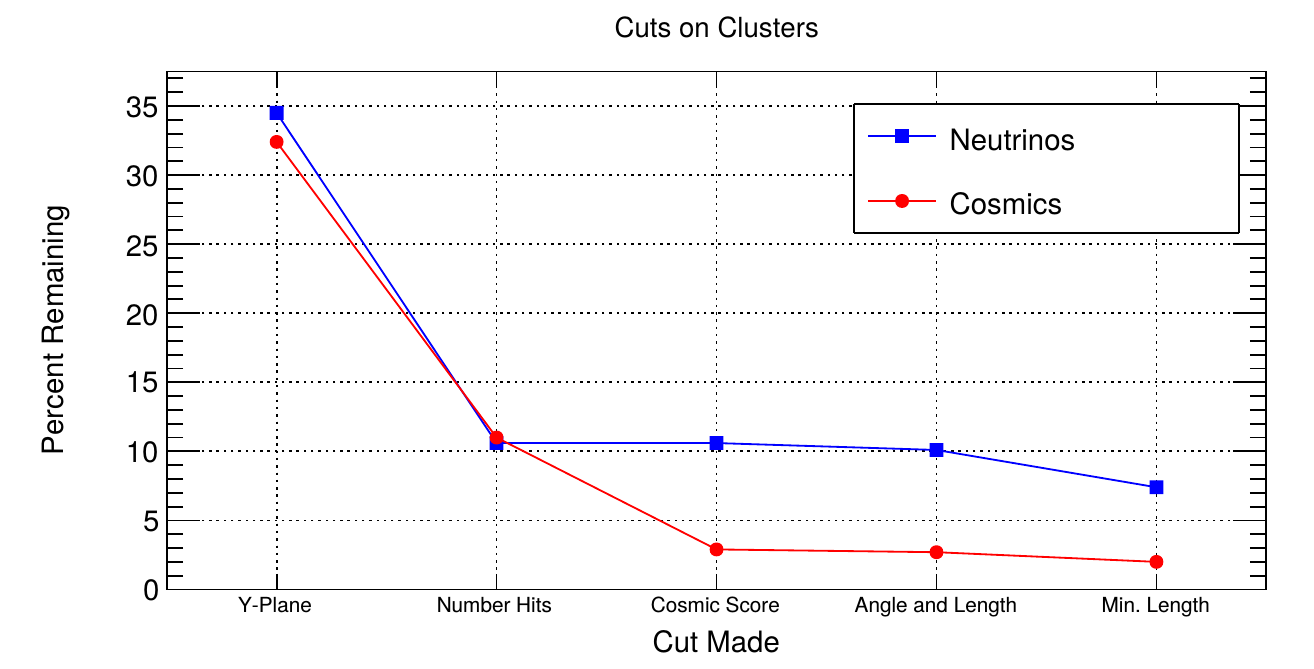
\includegraphics[width=\textwidth]{figs/2dprimarycut.png}
\caption{Percent of good clusters remaining for neutrinos and cosmics after the primary cuts were applied. This is relative to total number of initial clusters.}
\label{fig:2dprimarycut}
\end{figure}

\begin{figure}[htp!]
\centering
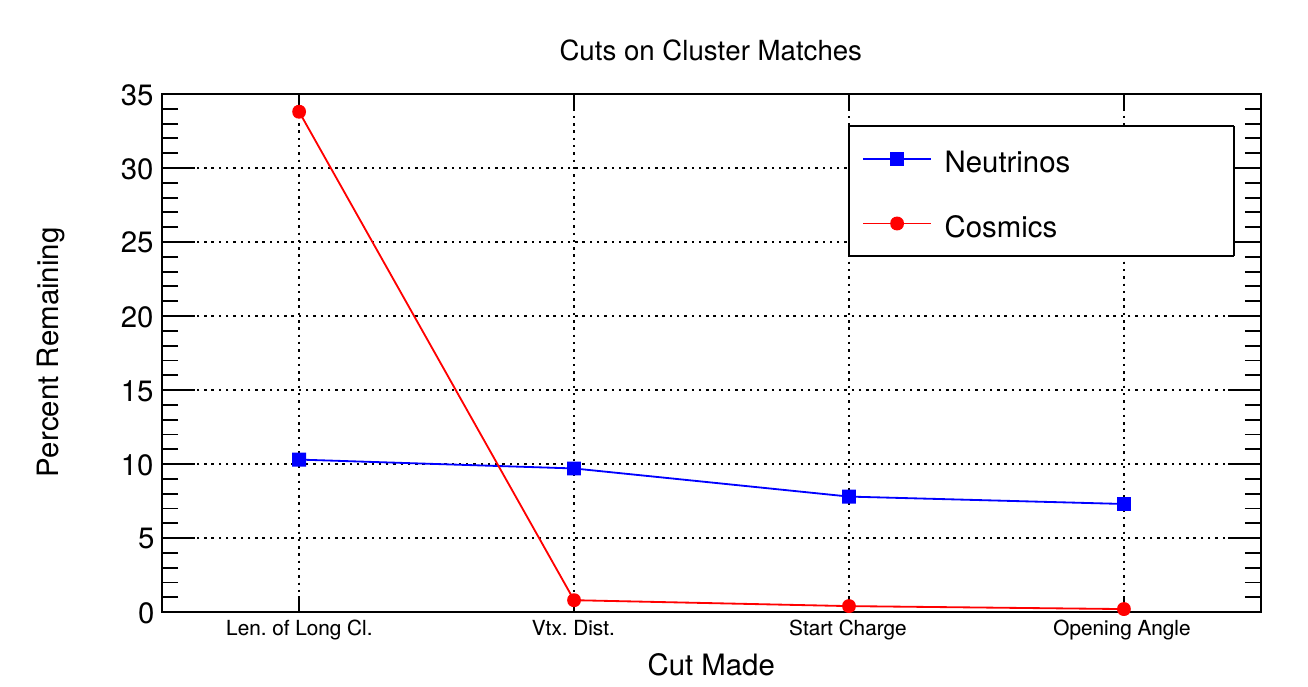
\includegraphics[width=\textwidth]{figs/2dsecondarycut.png}
\caption{Percent matched cluster pairs remaining for neutrinos and cosmics after secondary cuts applied. This is relative to the number of events that contain clusters which pass the primary cuts.}
\label{fig:2dsecondarycuts}
\end{figure}

\subsection{3D Tracks and vertices Selection}
The neutrino selection for the 3D channel was based on a reconstructed vertex and two tracks. All vertices and tracks were looped over that had a cosmic tag score < 0.4 and the distances below were calculated:
\begin{itemize}
\item d: distance between the start points of the two tracks.
\item $d_1$: distance between vertex and start of track 1.
\item $d_2$: distance between vertex and start of track 2.
\end{itemize}
The maximum distance of all three is then selected as the important characteristic per trio. The best trio is the one that has the smallest maximum distance. The $min(max_{d})$ for all trios in an event were plotted for BNB neutrino events and for cosmics to find the best cut value for each tracking algorithm. The distribution of $min(max_{d,i})$ is smaller for neutrinos than for cosmics. The cut values for different tracking and clustering algorithms are shown below. These cut values were chosen to minimize the cosmic background to 20\%. 
\begin{itemize}
\item trackkalmanhit with cccluster $min(max_{d,i})$ < 3 cm.
\item trackkalmanhit with pandoraNu $min(max_{d,i})$ < 4.5 cm.
\item pandoraNu with cccluster $min(max_{d,i})$ < 5 cm.
\end{itemize}

\subsection{TPC Updates}
After doing a visual hand-scanning of the first beam data processed with the filters detailed above, the events passing had a larger contamination of background than expected. This was mainly due to the reconstruction performing better on simulation than on data. Due to this, additional cuts on both streams needed to be implemented in order to increase signal/background ratio. These cuts were added on top of the filters described above and further reduce the event count. 
\subsubsection{2D Filter Updates}
The main background observed in the 2D filter were Michel events, where the muon and electron formed two connected clusters. These events were rejected by comparing the start and end charge deposition of the long cluster (i.e muon particle). The start charge deposition must be less than the end charge deposition. This cut is implemented because muons have a higher ionization loss at the end. 
\subsubsection{3D Filter Updates}
It was seen that cosmic tracks can often originate or end at the same point, therefore faking a signal. Cosmic tracks, however, are mostly vertical. By requiring the angle of the longer track have a cosine greater than 0.85 with respect to the z-axis as well as requiring the longer track to have a length greater than 10 cm, we can reduce this background. 
\section{Conclusion}
After processing these filters in parallel, it was shown that the 3D filter had a higher purity than the 2D filter because of the higher cosmic rejection being used due to 3D reconstruction. The 2D filter is blind to track entering/exiting from the top or bottom of the TPC. Although the 3D filter had a higher purity, the 2D filter was still able to find identifiable events in data that were used as public event displays. A sample of event displays are shown in figures \ref{fig:2dimage} and \ref{fig:3dimage}.

\begin{figure}[htp!]
\centering
	\begin{subfigure}[b]{.8\textwidth}
	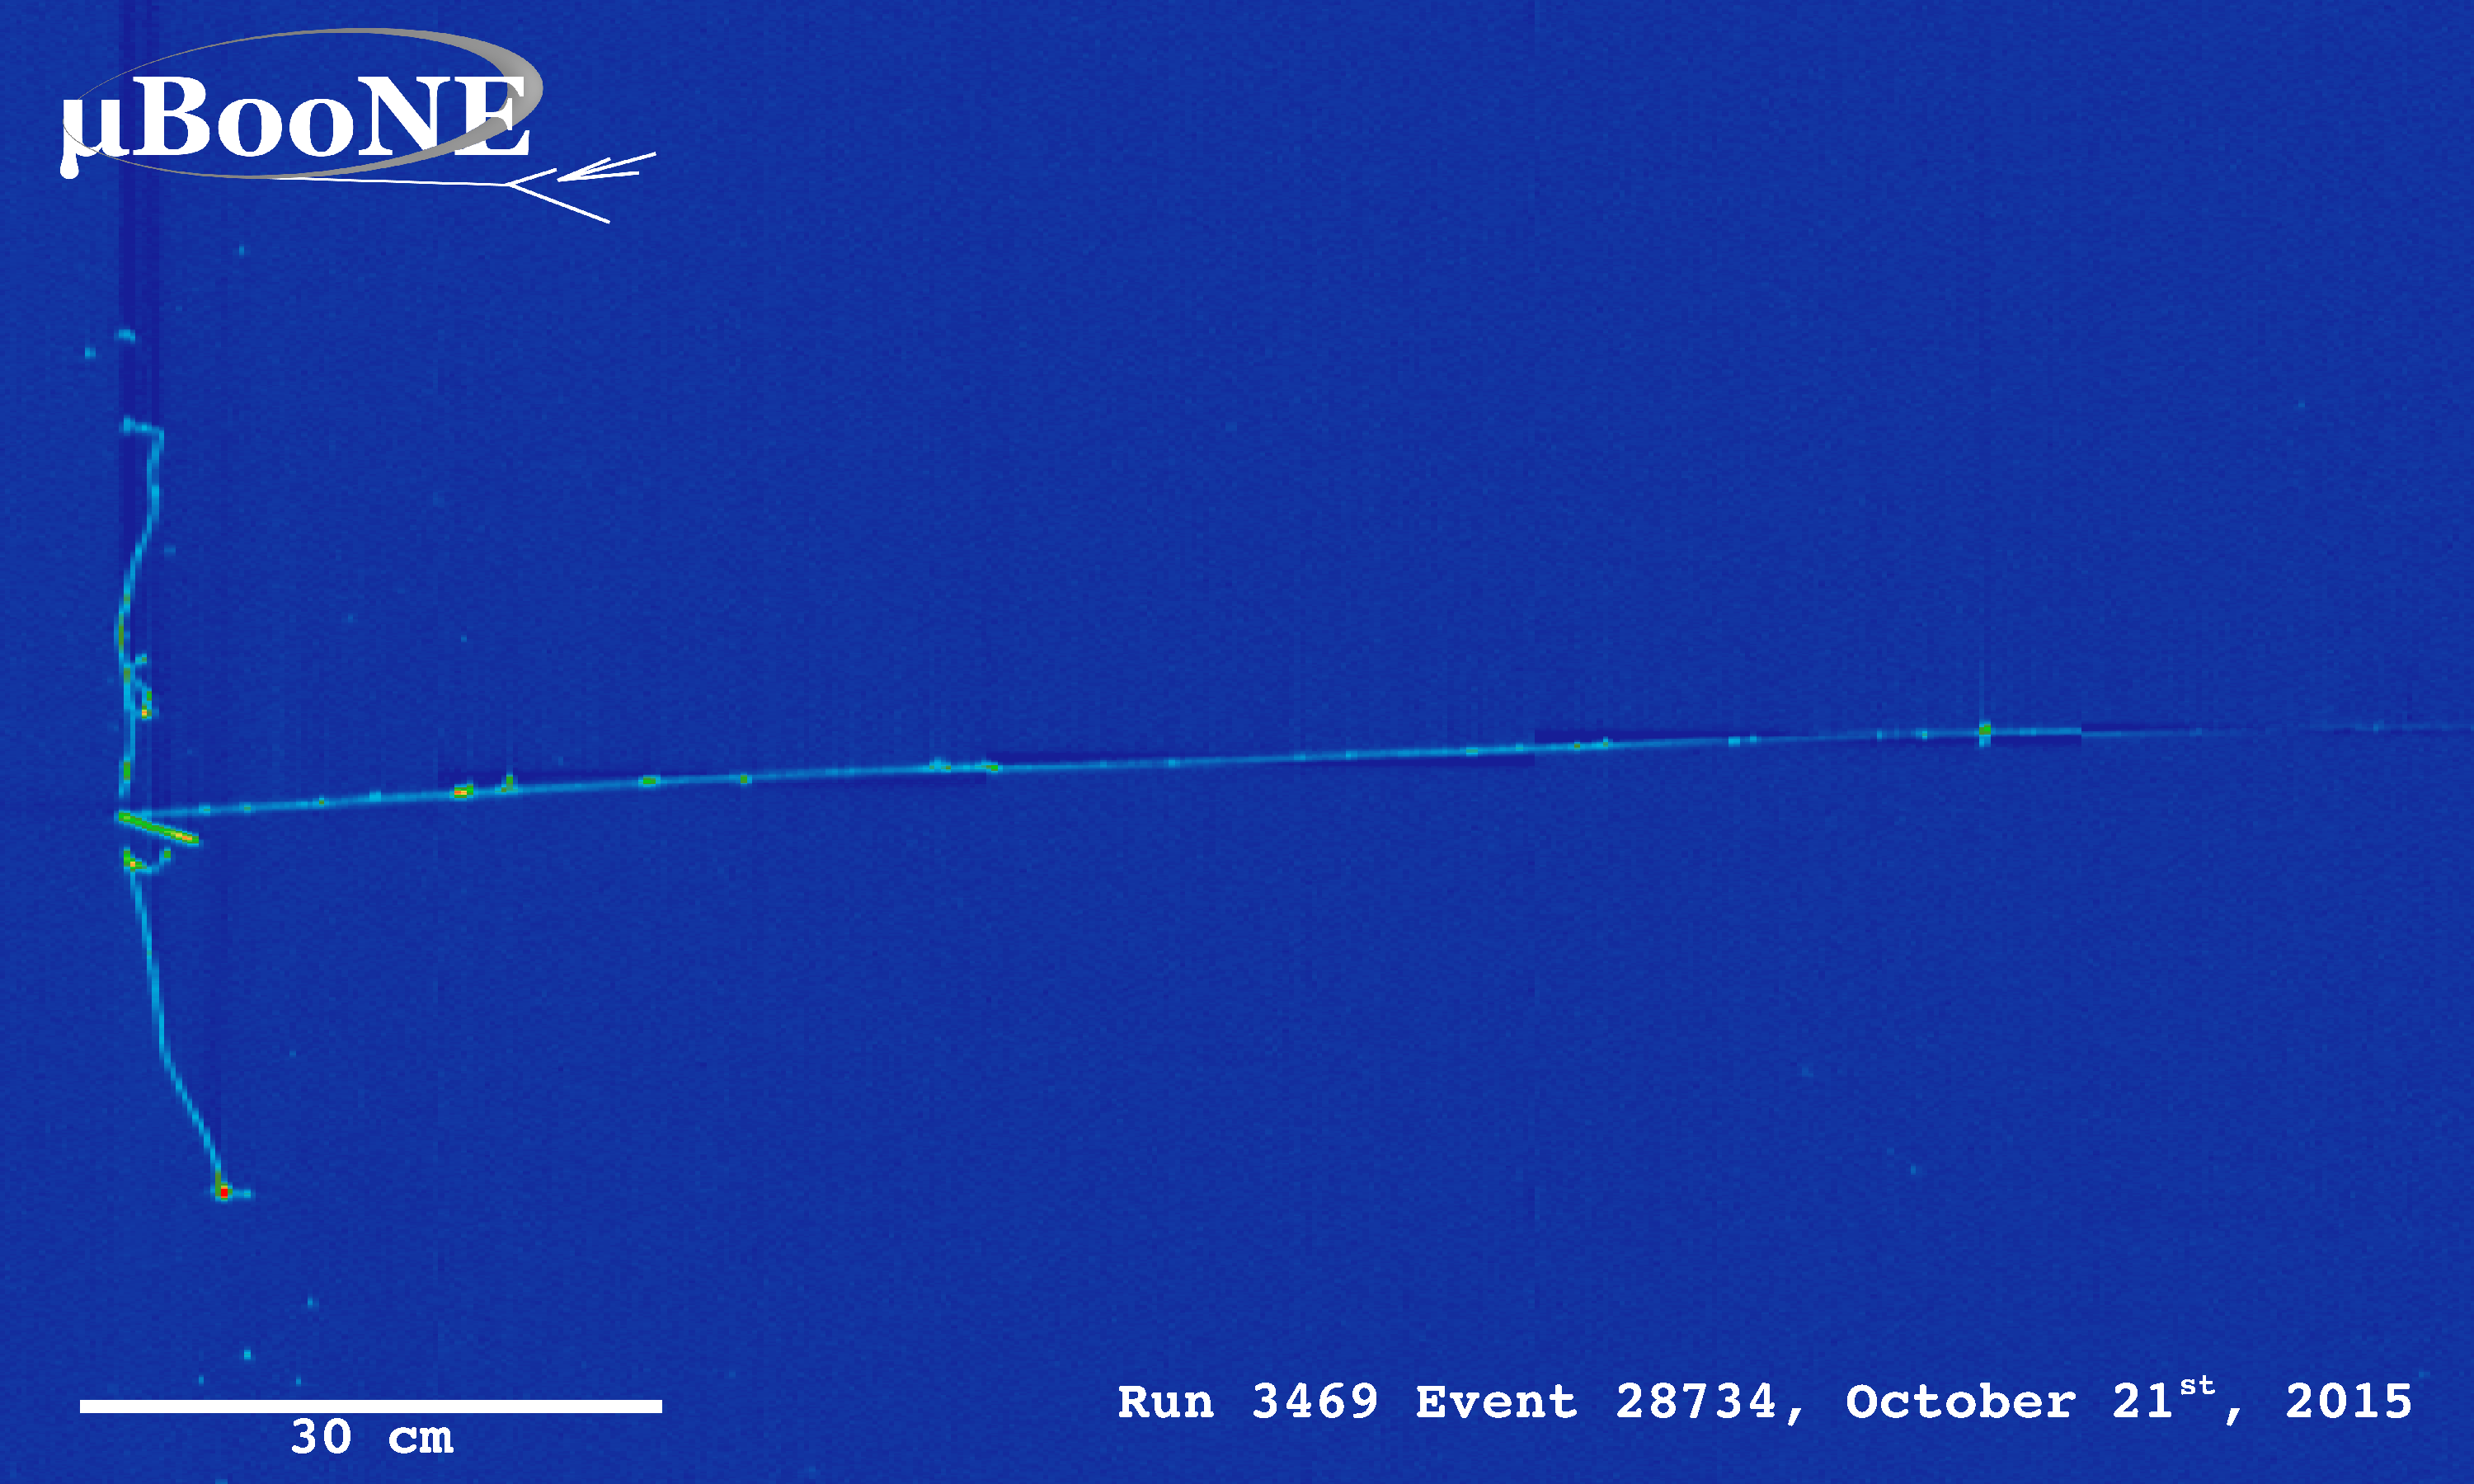
\includegraphics[width=\textwidth]{figs/first_neutrino_pdfs/run3469_subrun574_event28734_col.pdf}
	\end{subfigure}
	\quad
	\begin{subfigure}[b]{.8\textwidth}
	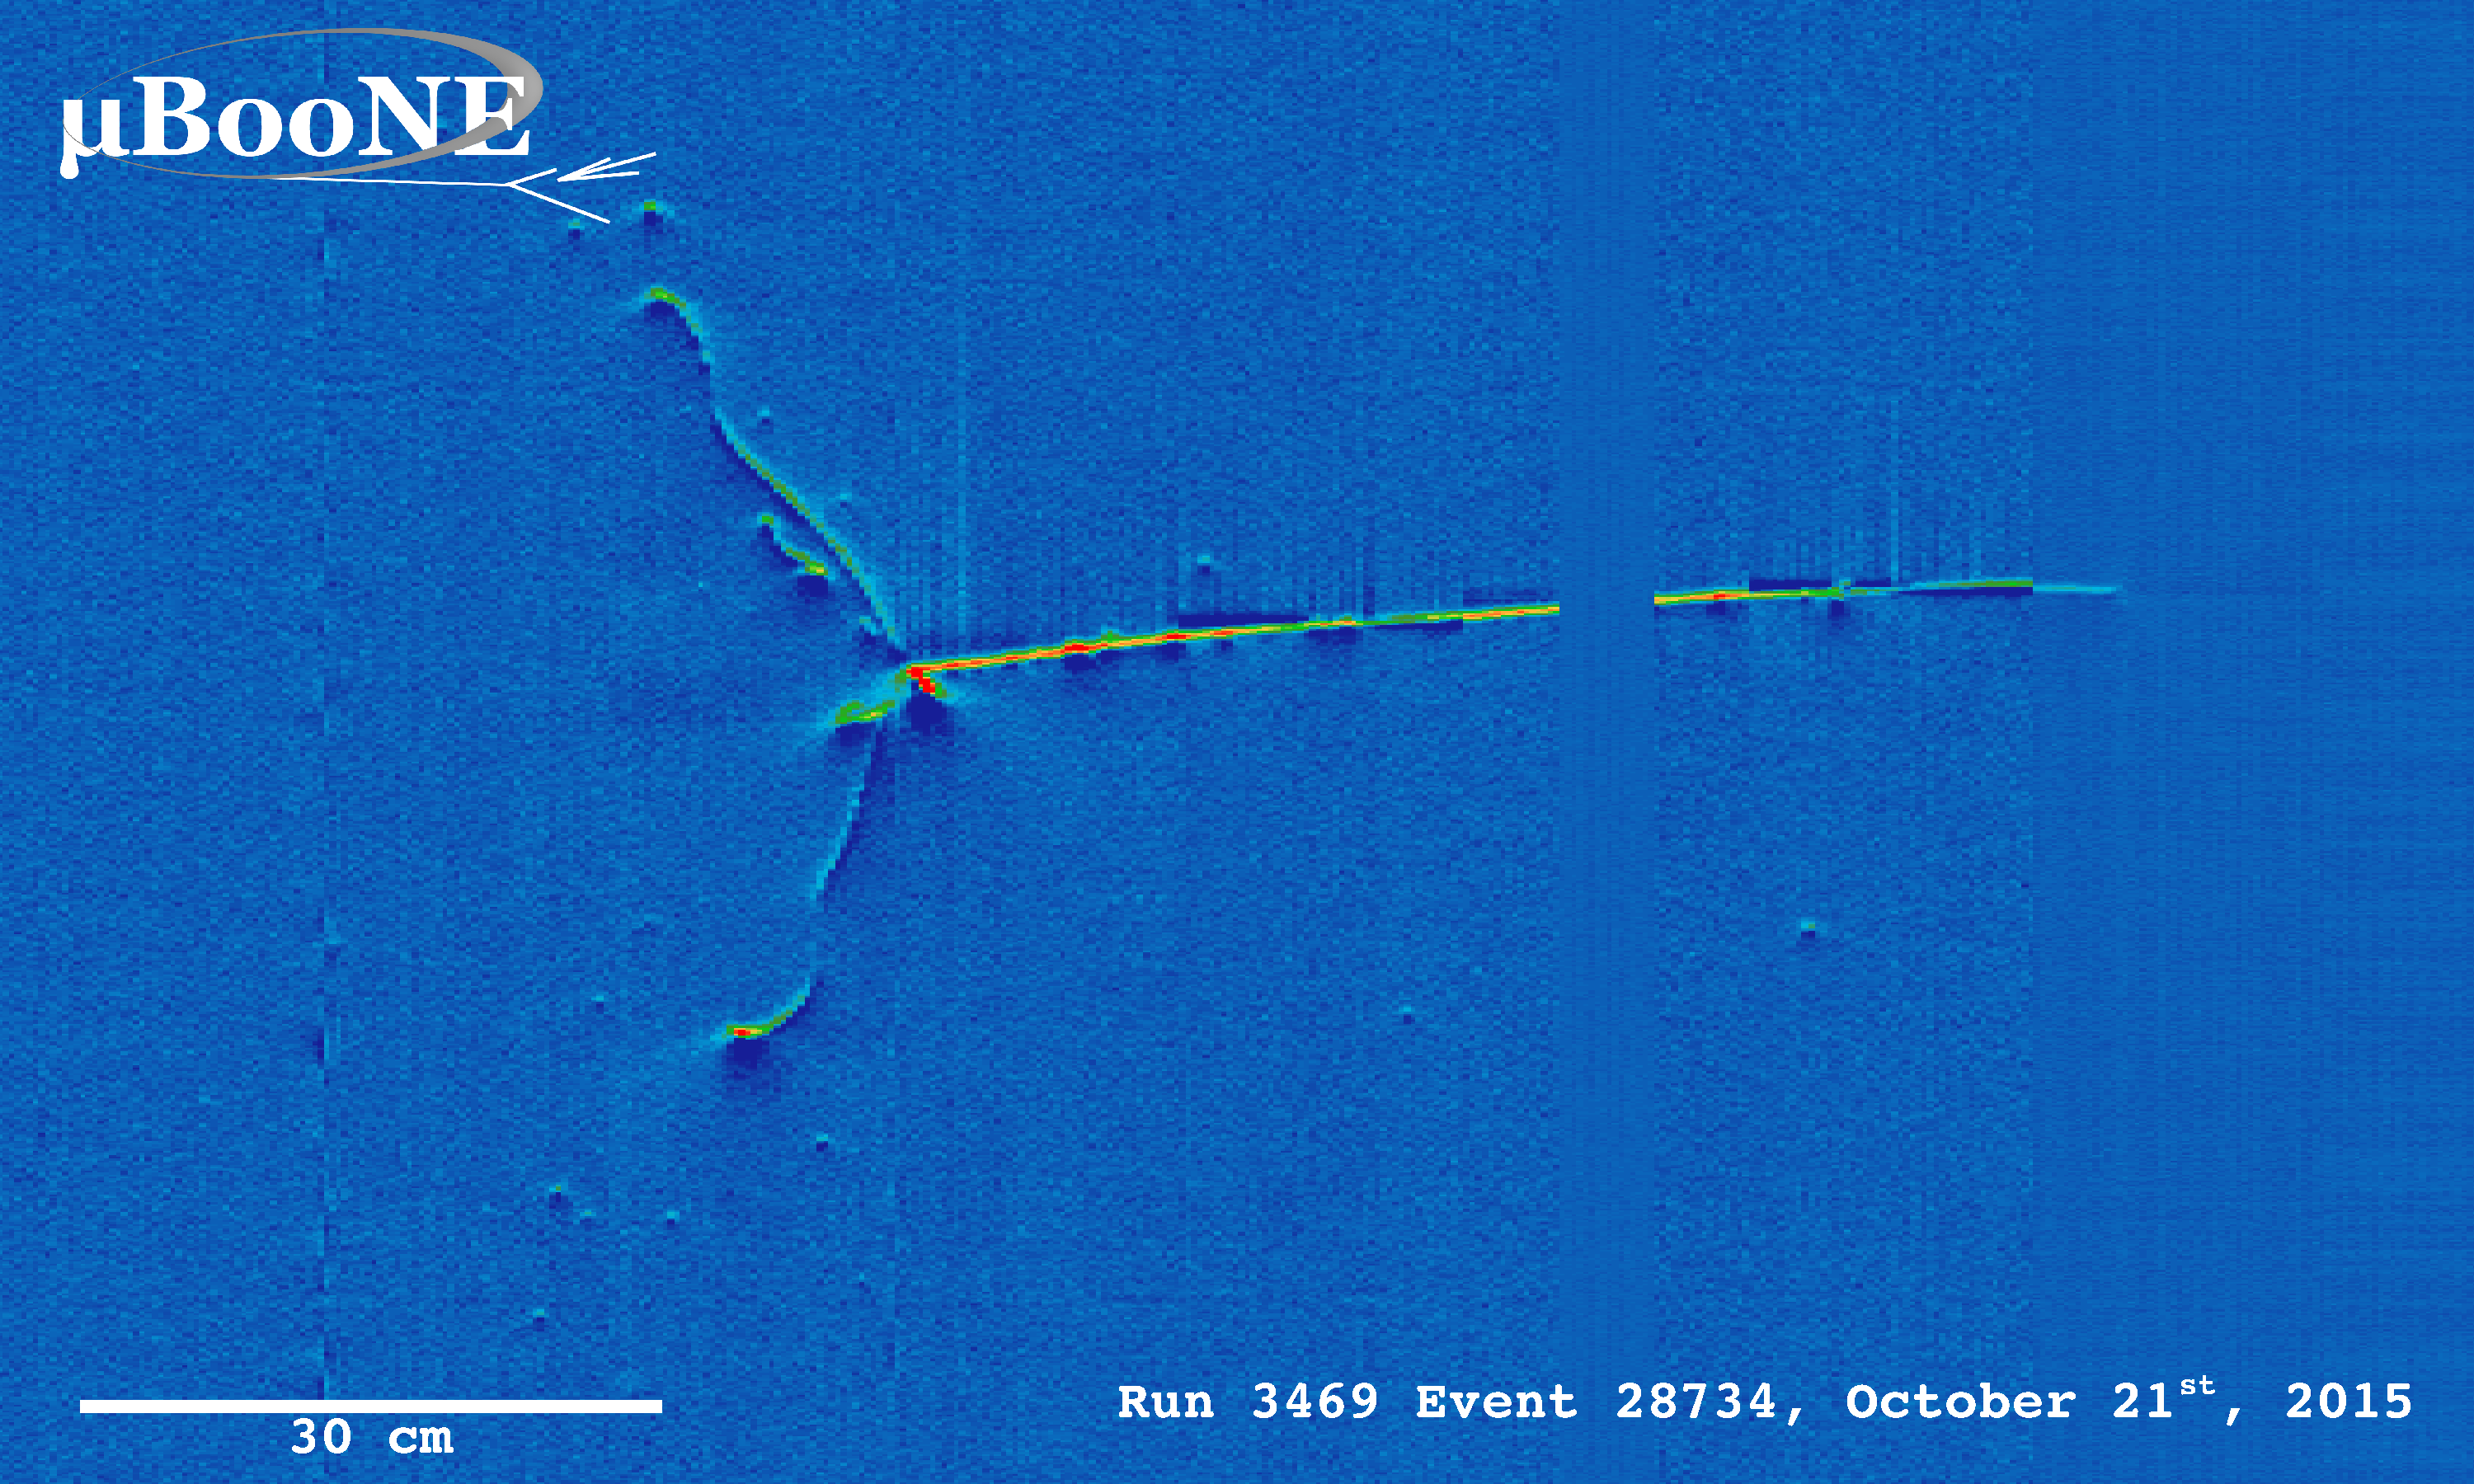
\includegraphics[width=\textwidth]{figs/first_neutrino_pdfs/run3469_subrun574_event28734_ind0.pdf}
	\end{subfigure}
	\quad
	\begin{subfigure}[b]{.8\textwidth}
	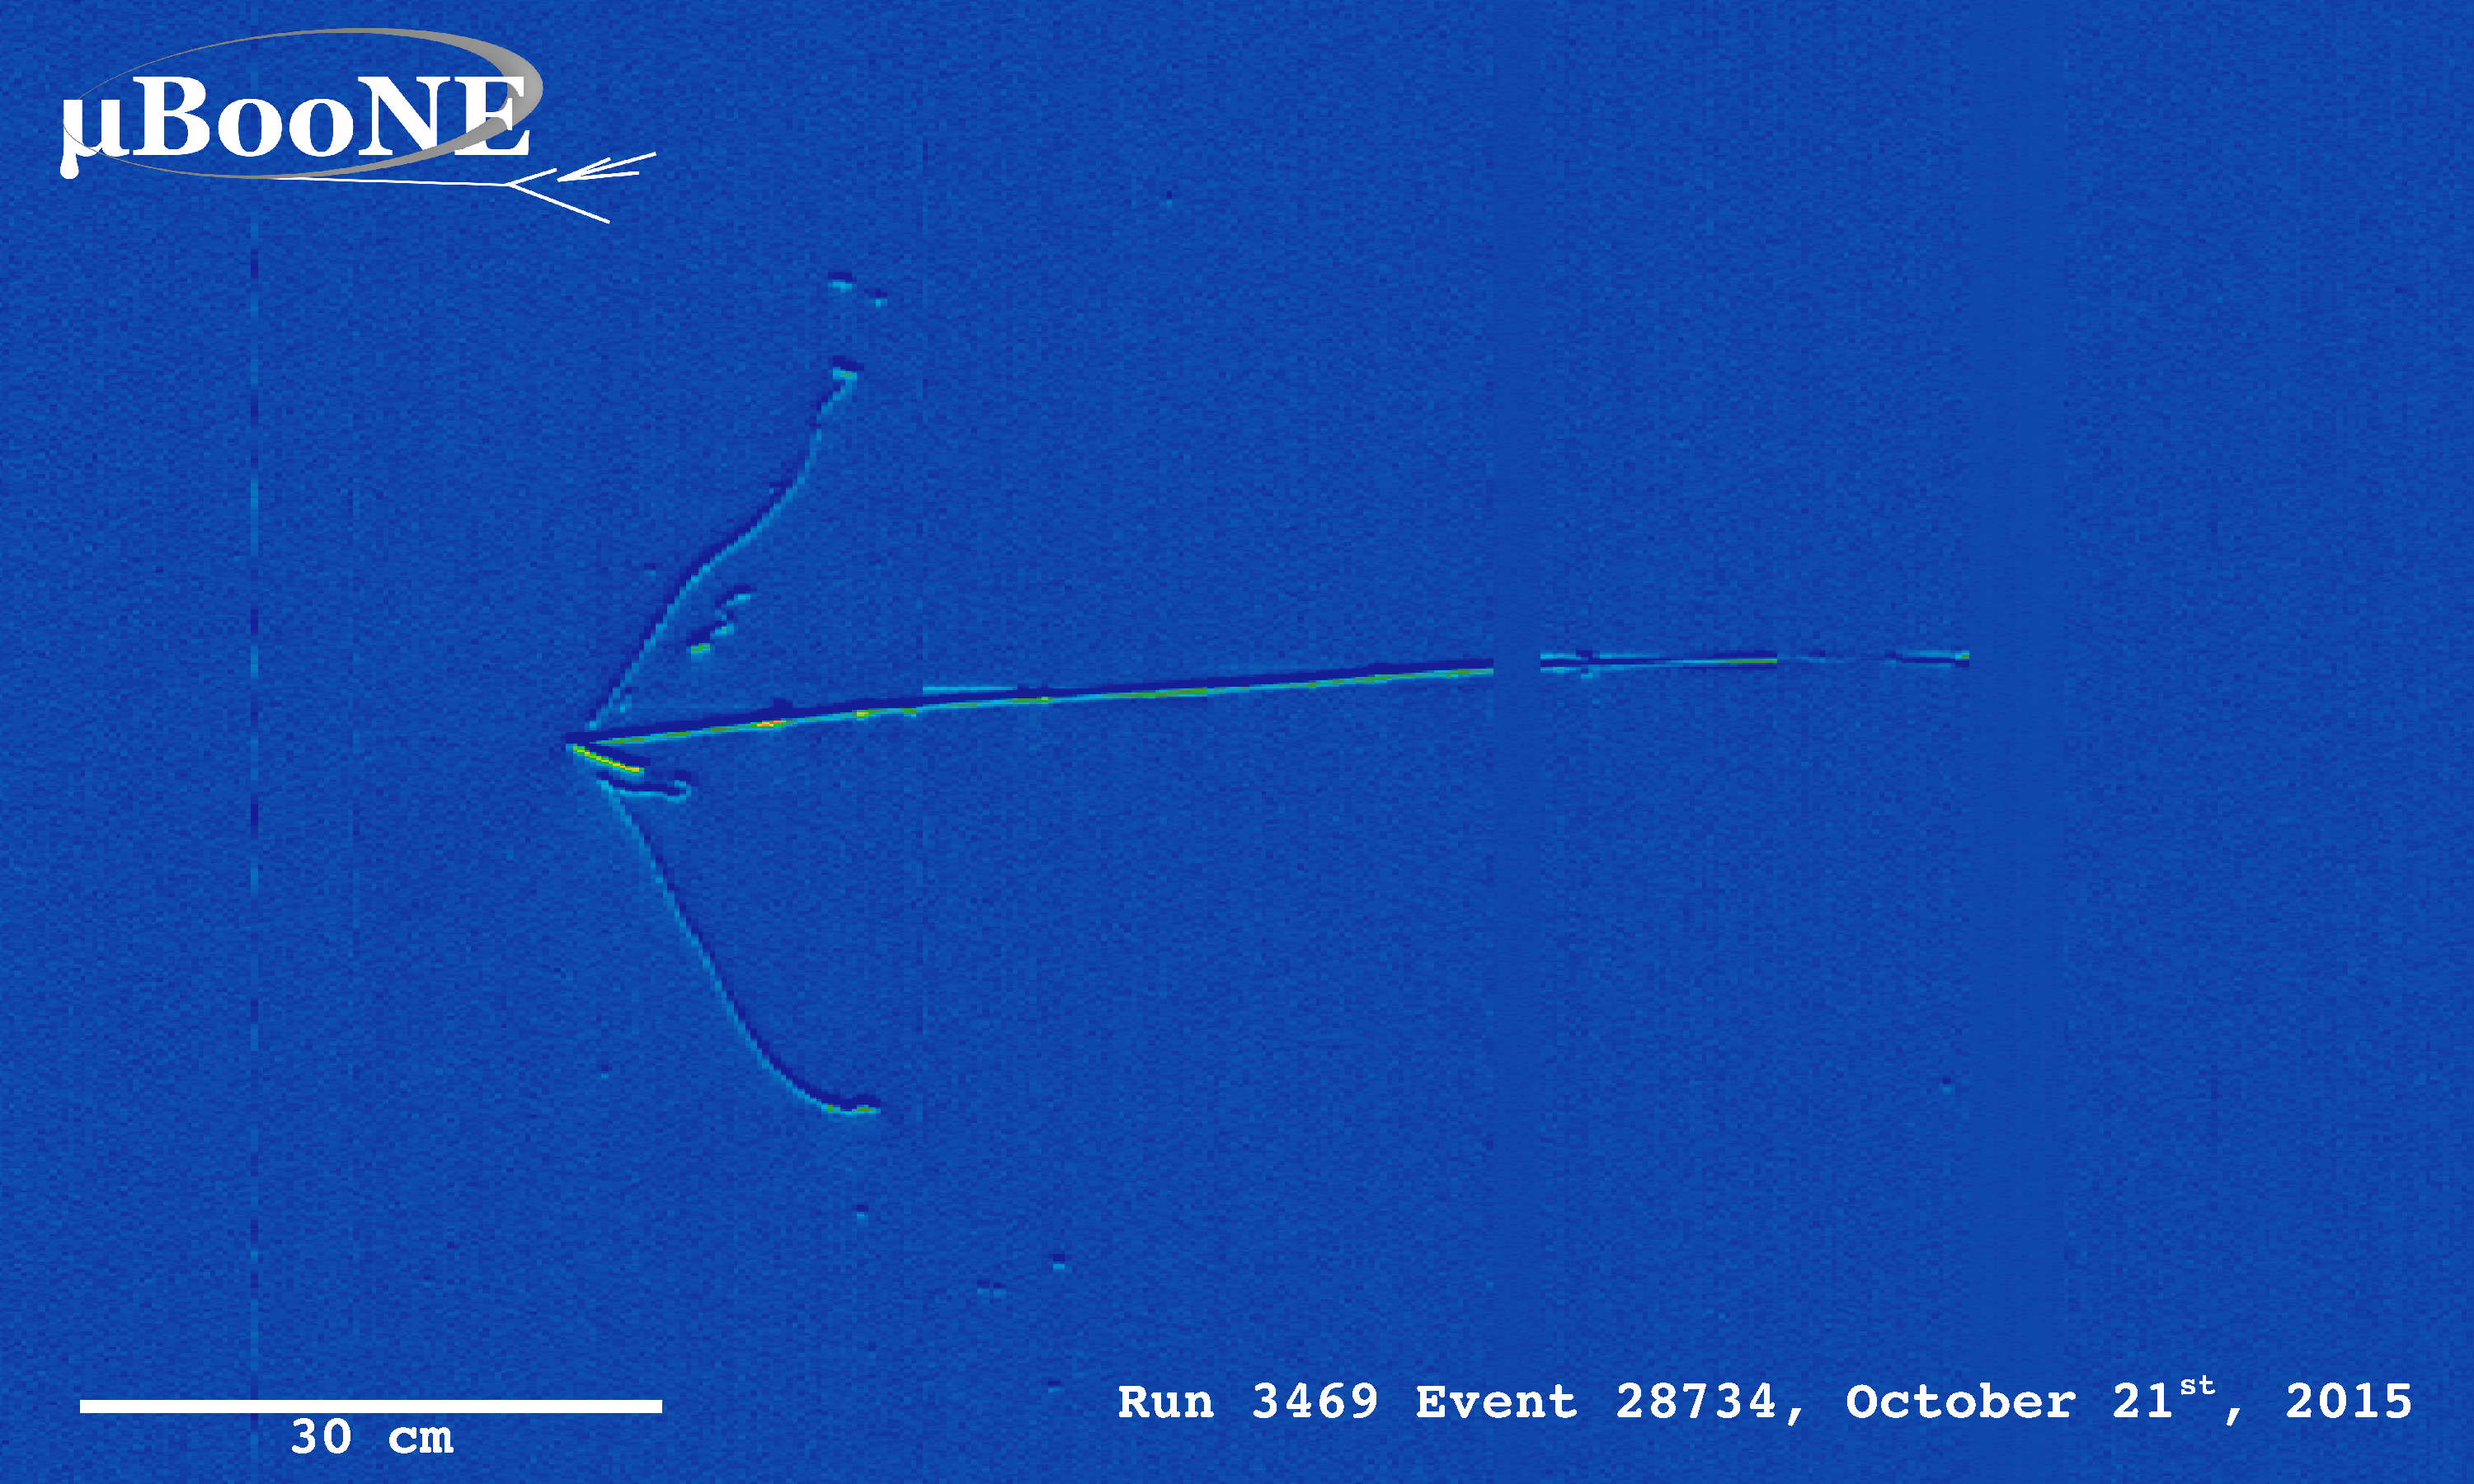
\includegraphics[width=\textwidth]{figs/first_neutrino_pdfs/run3469_subrun574_event28734_ind1.pdf}
	\end{subfigure}
	\quad
\caption{First Neutrino Interaction Candidate Events from MicroBooNE}
\label{fig:2dimage}
\end{figure}

\begin{figure}[htp!]
\centering
	\begin{subfigure}[b]{.8\textwidth}
	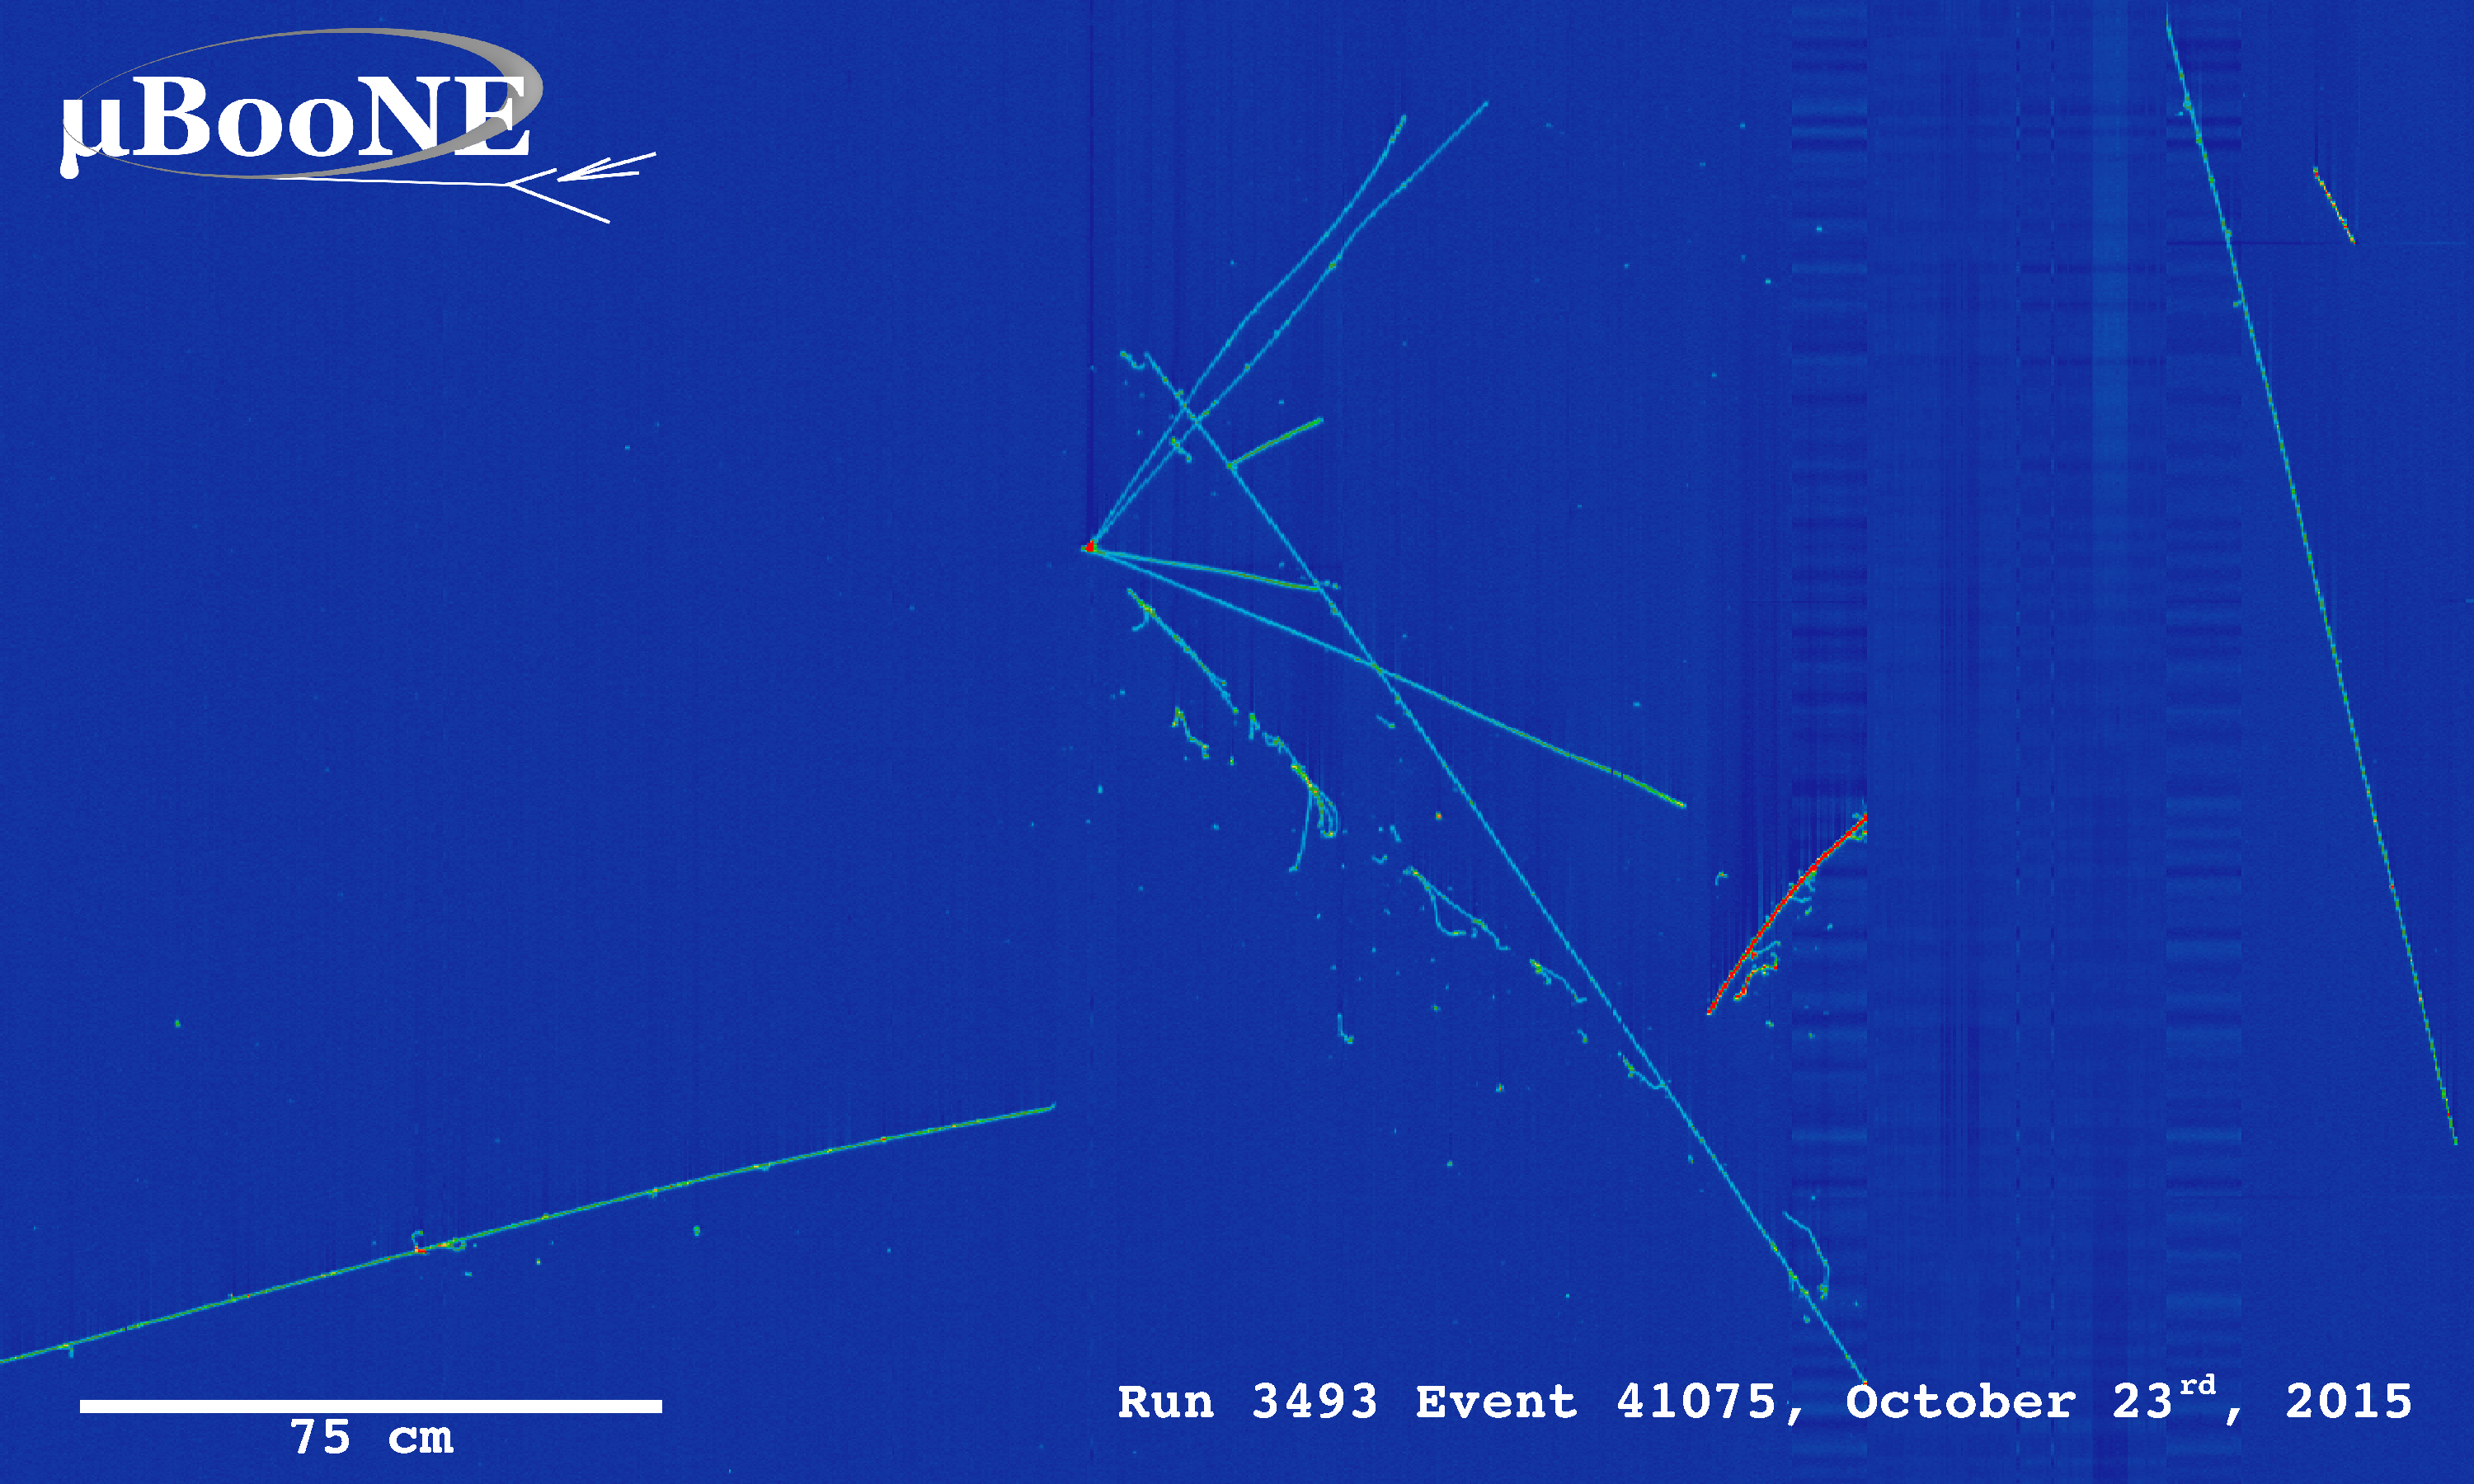
\includegraphics[width=\textwidth]{figs/first_neutrino_pdfs/run3493_subrun821_event41075_col.pdf}
	\end{subfigure}
	\quad
	\begin{subfigure}[b]{.8\textwidth}
	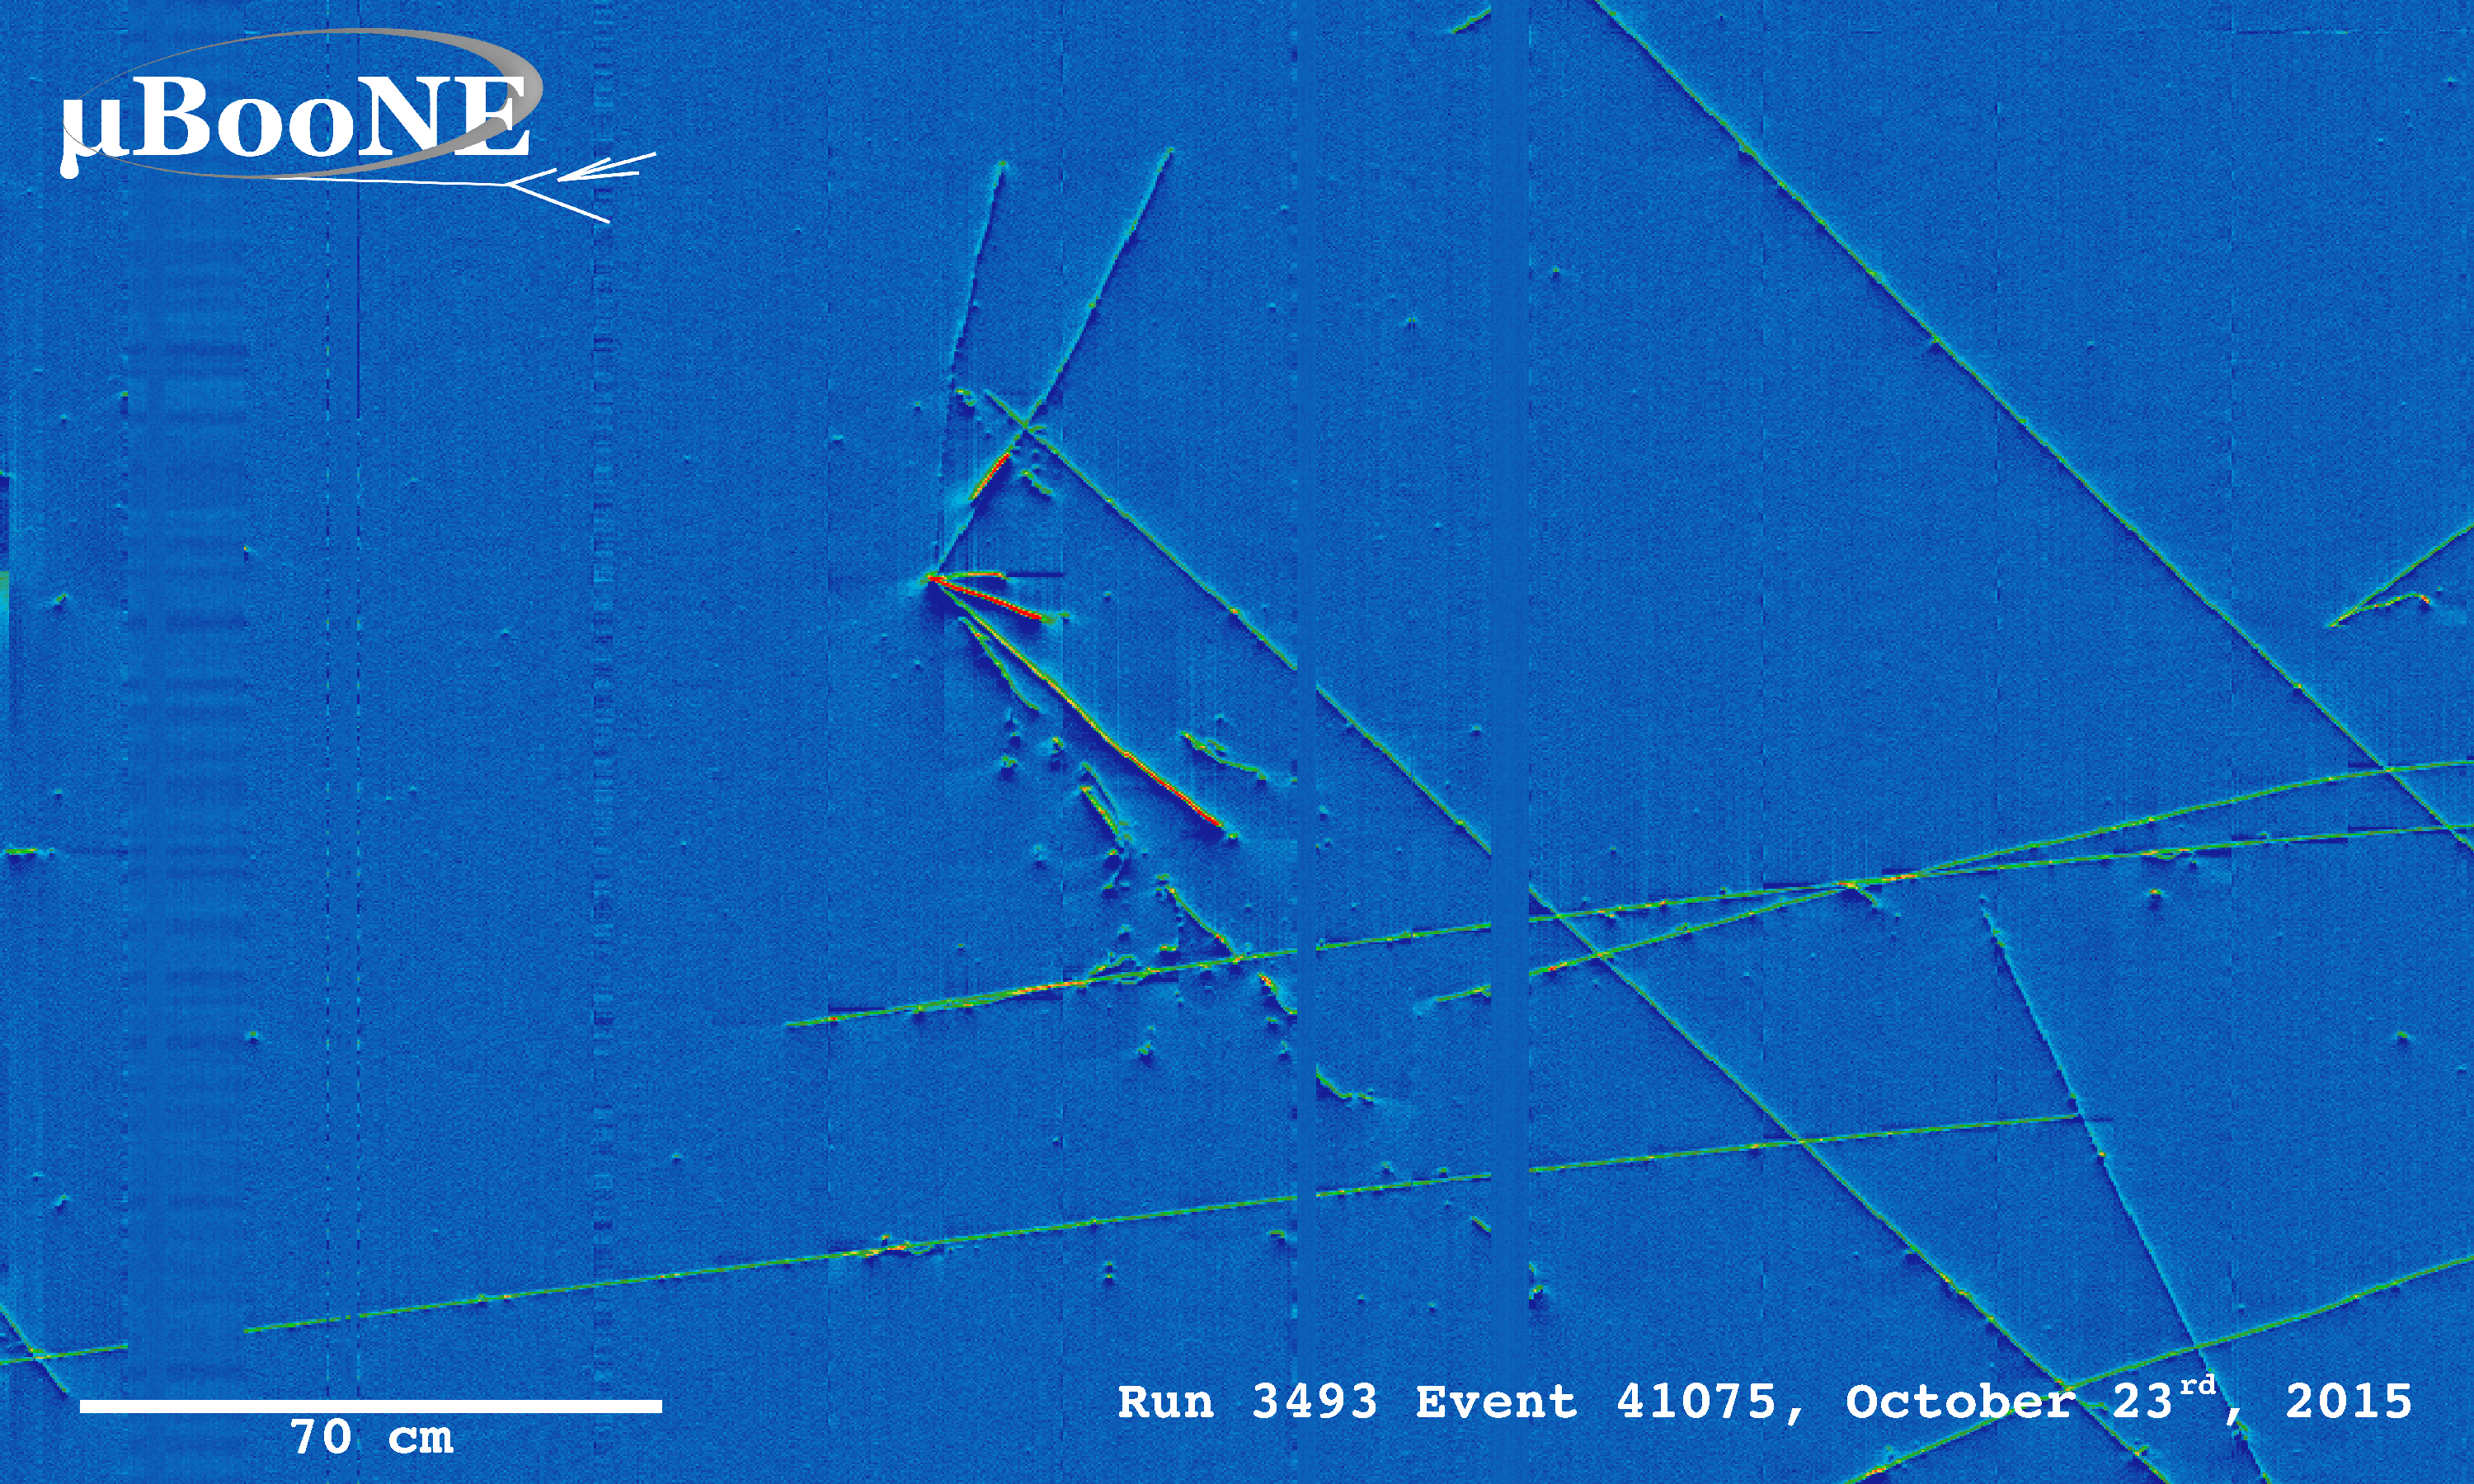
\includegraphics[width=\textwidth]{figs/first_neutrino_pdfs/run3493_subrun821_event41075_ind0.pdf}
	\end{subfigure}
	\quad
	\begin{subfigure}[b]{.8\textwidth}
	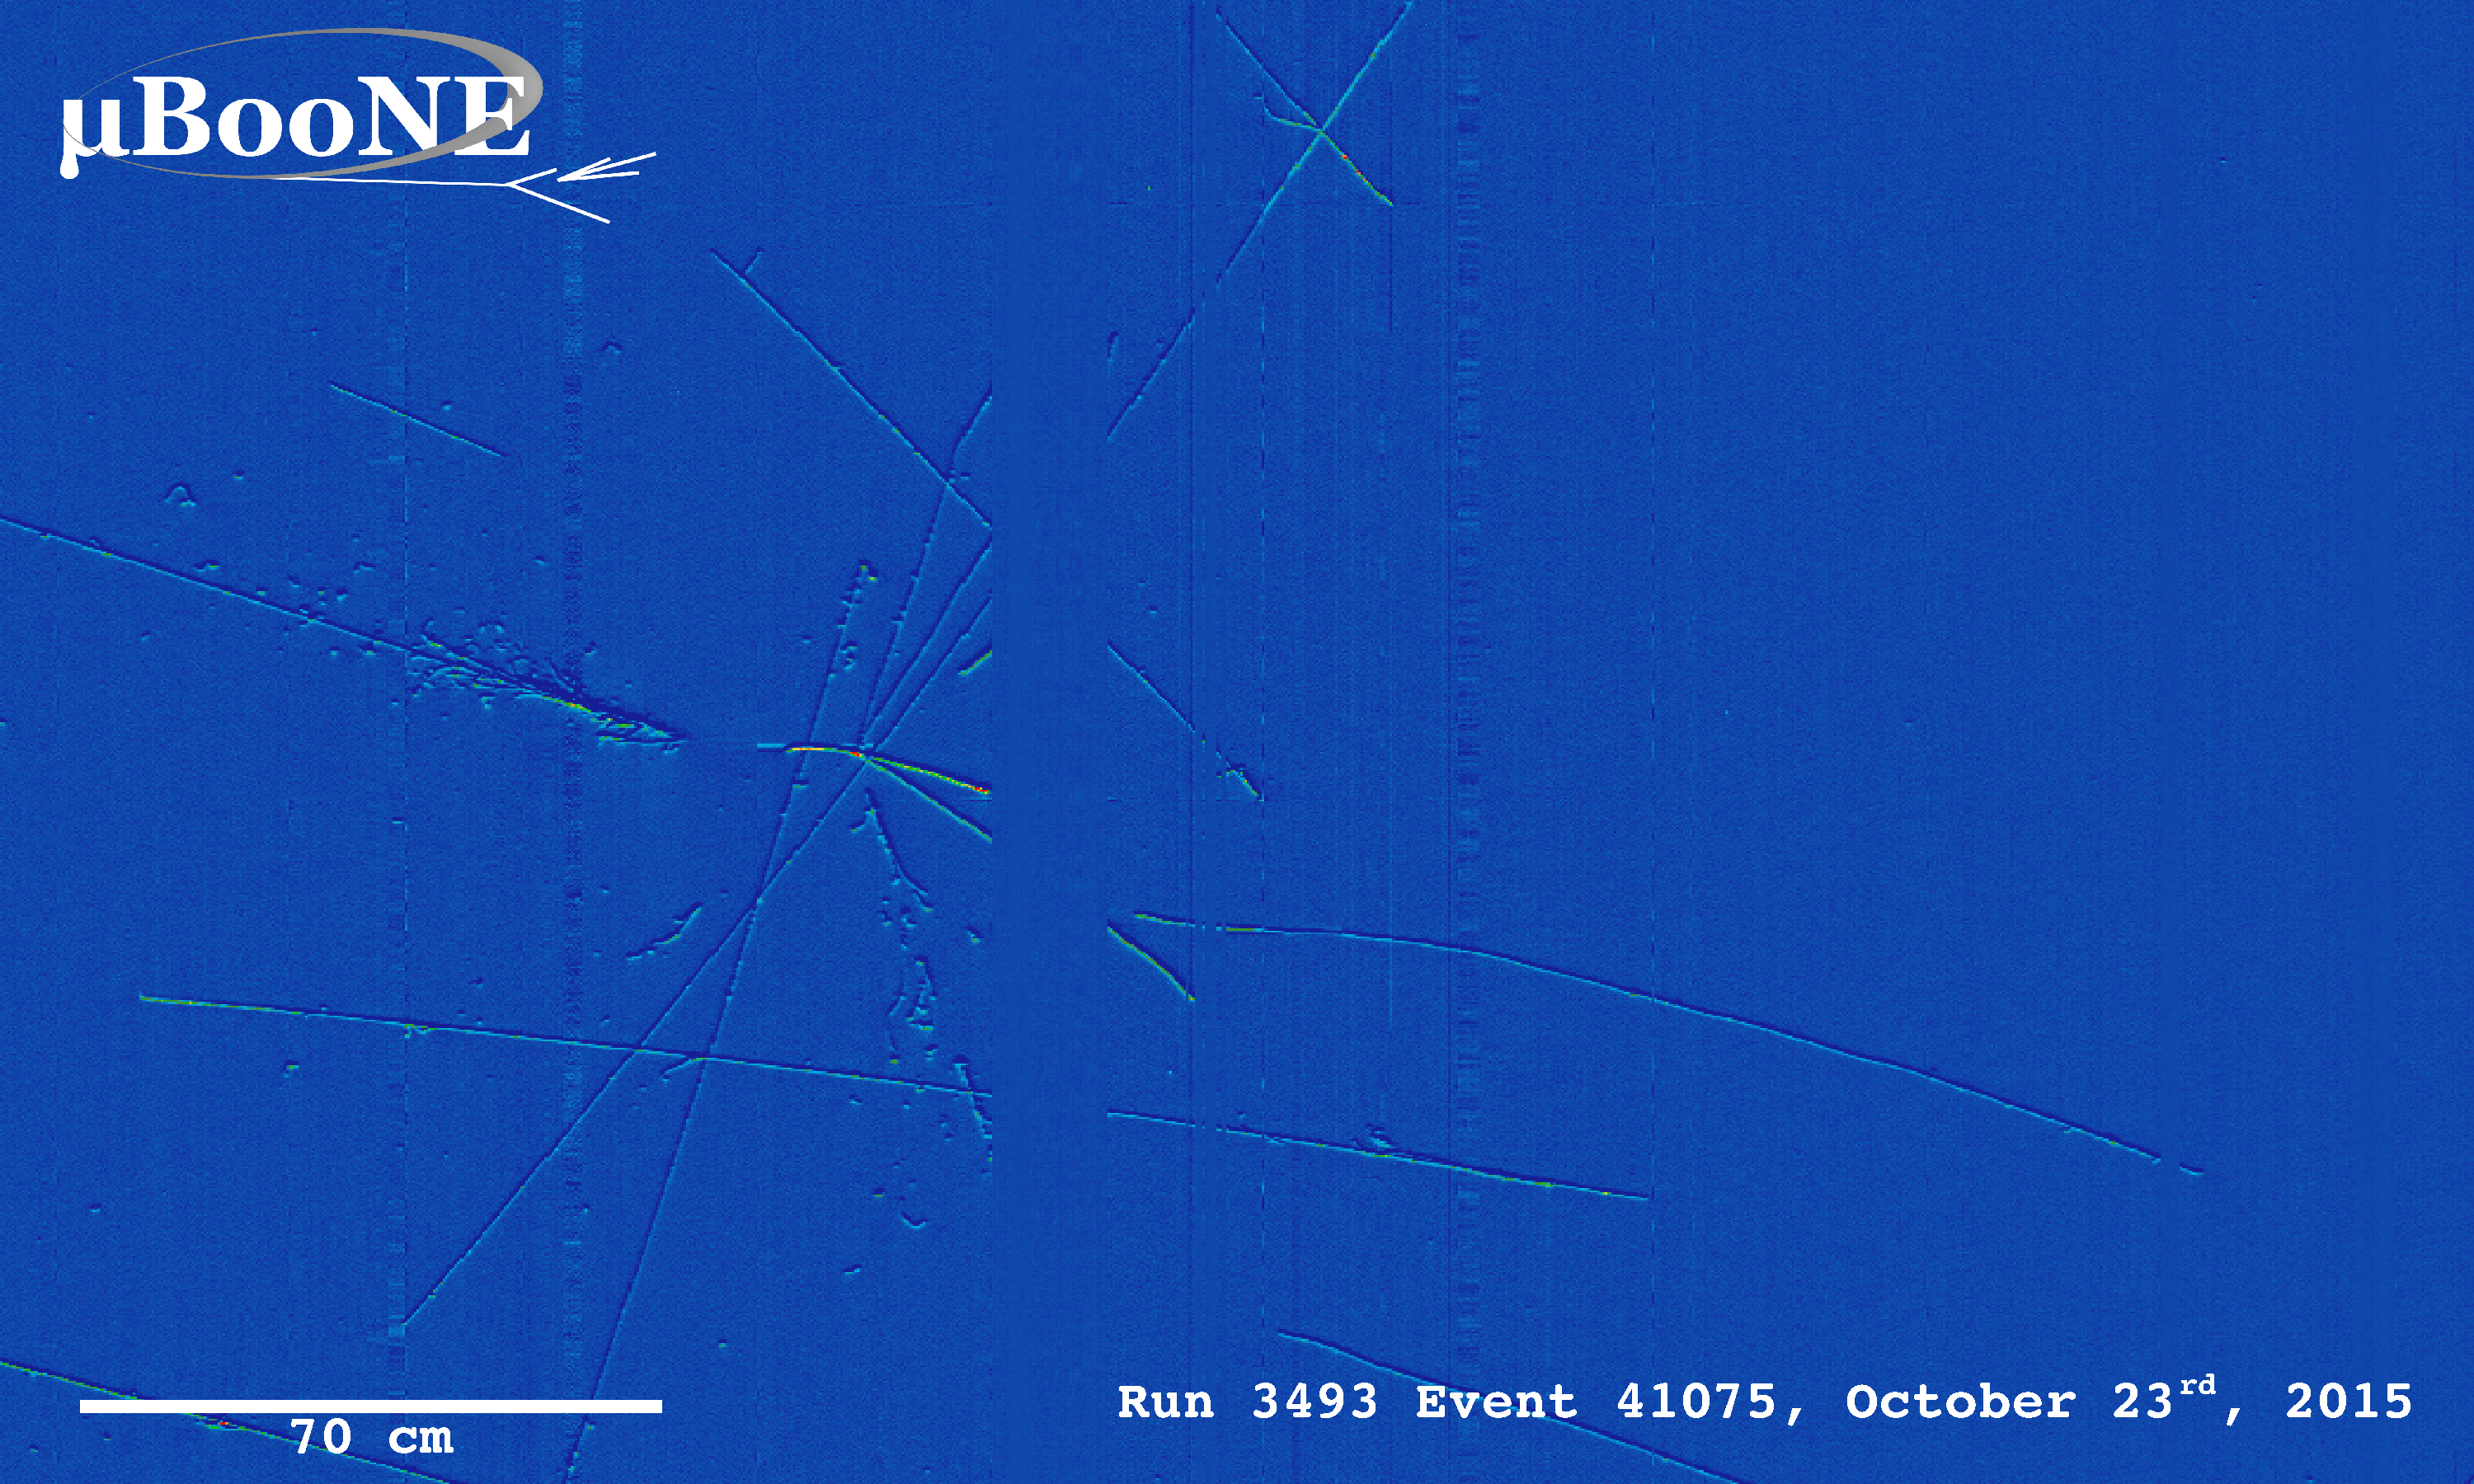
\includegraphics[width=\textwidth]{figs/first_neutrino_pdfs/run3493_subrun821_event41075_ind1.pdf}
	\end{subfigure}
	\quad
\caption{First Neutrino Interaction Candidate Events from MicroBooNE}
\label{fig:3dimage}
\end{figure}

  \chapter{CC-Inclusive Cross Section Selection Filter} \label{ch:meas}
The CC-Inclusive cross-section selection I and selection I modified filters used in this analysis will be described in the following sections below. These filters are an expansion of the Neutrino ID filter. The work done in this thesis was to further improve these selections by increasing both efficiency and purity as well as increasing acceptance without further affecting the kinematic distributions of the selected neutrino events.
 
MicroBooNE requires fully automated event reconstruction and selection algorithms for use in the many physics measurements being worked on to date due to the large data rate MicroBooNE receives. Being able to automatically pluck out the neutrino interaction among a sea of cosmics proved to be challenging but was accomplished. MicroBooNE has developed two complementary and preliminary selection algorithms to select charged-current $\nu_{\mu}-Ar$ interactions. Both are fully automated and cut based. The results of this thesis will focus on selection I and selection I modified and will focus on further improving these algorithms using Convolutional Neural Network (CNN) implementations. These selections identify the muon from a neutrino interaction without biasing towards track multiplicity. To combat cosmic and neutral current background, the analysis is strongly biased towards forward-going long tracks which are contained. This limits phase space and reduces acceptance. 

\section{Data and MC Processing Chain}
The data used for this analysis were based on hardware and software triggers. Events used came from the \textit{BNB\_INCLUSIVE} and \textit{EXT\_BNB\_INCLUSIVE} streams and were used for signal and background. The \textit{BNB\_INCLUSIVE} stream is chosen by requiring that the hardware trigger bit is fired and that the event passed an optical software trigger within a BNB spill timing window. The \textit{EXT\_BNB\_INCLUSIVE} stream requires the EXT hardware trigger to fire as well as pass the same optical software trigger within a BNB spill size timing window similar to the \textit{BNB\_INCLUSIVE}. 

The two MC samples used in this analysis and for determining selection efficiencies and purities were GENIE BNB neutrino interactions with CORSIKA cosmic ray overlay within the readout window and inTime CORSIKA cosmic rays. The MC samples generated used \textit{\textbf{uboonecode v04\_36\_00}} and are based on the following packages:
\begin{itemize}
\item{larsoft v04\_36\_00}
\item{GEANT v04\_09\_06\_p04d}
\item{GENIE v02\_08\_06d}
\item{GENIE xsec v02\_08\_06a}
\item{pandora v02\_03\_0a}
\item{CORSIKA v07\_4003}
\end{itemize}

Both data and MC samples were processed using the same reconstruction release, \textit{\textbf{uboonecode v05\_08\_00}} and the fcl files used for reconstruction are listed below:
\begin{itemize}
\item{MC fcl files}
\begin{itemize}
\item{reco\_uboone\_mcc7\_driver\_stage1.fcl}
\item{reco\_uboone\_mcc7\_driver\_stage2.fcl}
\end{itemize}
\item{Data fcl files}
\item{reco\_uboone\_data\_Feb2016\_driver\_stage1.fcl}
\item{reco\_uboone\_data\_Feb2016\_driver\_stage2.fcl}
\end{itemize}

On top of the hardware and software triggers, the data also had to pass more criteria to be identified as part of the good run list. The criteria is detailed below.
\begin{itemize}
\item{\textbf{Detector conditions:} the detector has to be in a good operating condition. The detector conditions are read from the slow monitoring database and are required to be within the alarm thresholds. The variables of interest for events passing the good run list criteria include DAQ, PMT, HV, Drift HV, wire bias, electron lifetime and detector power. These conditions need to be met on a run-by-run basis in order to pass the selection.}
\item{\textbf{Data quality:} normal and stable behavior for basic reconstruction quantities. These reconstruction variables include average number of tracks, hits, and flashes in each event, the average length of tracks, the average amplitude and area of hits, the average PE and the average spread of each one of these quantities.}
\item{\textbf{Beam Conditions:} the BNB must be on and stable and the POT per spill needs to above the intensity threshold. Beam quality conditions include checking the fraction of proton beam interacting within the target, the horn current, and the intensity of protons per spill. The final sample is $5 * 10^{19}$ and a per-spill intensity of $4 * 10^{12}$}
\item{\textbf{Run processed:} the full run must be processed completely without missing subruns or crashes in the data processing.}
\end{itemize}

The selection begins with a cut that requires an optical flash greater than 50 photo electrons (PE) in the 1.6 $\mu$s beam window. Next, two or more 3D reconstructed tracks must be within 5 cm from a 3D reconstructed vertex. The most forward going track vertex-track association is then selected for further cuts. The vertex from the chosen association must be in the fiducial volume, and the longest track from this association must be matched to a flash 80 cm in z. Lastly the longest track must be contained and longer than 75 cm.       

\section{Normalization of data and MC}
The off-beam sample is used to measure beam unrelated backgrounds. For normalization, one needs the total number of BNB spills \textit{$(N_{BNB}$} and the total number of external triggers. The BNB spills used need to pass the beam quality cuts. The normalization factor is then \textit{$N_{BNB}/N_{EXT}$} which is 1.23. 

To normalize generated BNB MC events to POT, we used the following:
\begin{itemize}
\item{ $5 * 10^{19} POT = 41524.3$ generated events}
\end{itemize}
where this scaling factor only applies to mcc7 generated events. The inTime cosmic sample is normalized with respect to the open cosmic sample so an understanding of both is necessary. The POT per beam spill for mcc7 BNB samples is $5 * 10^{12}$. To calculate how many spills are necessary to produce a specific POT one would multiply the total POT by the average 1/POT per spill. For a total POT of $5 * 10^{19}$ the amount of spills necessary is $\frac{5 * 10^{19}}{5 * 10^{12}} = 1 * 10^7$. This is only one in \sim 241 events therefore each cosmic event needs to be scaled up by a factor of 240.8 when comparing to BNB MC. For inTime cosmics however, two filters are applied to reduce computing and processing time and only leave cosmics that will interact within the detector. The passing rate after these two filters is 0.02125, therefore the total inTime cosmic scaling factor to compare inTime cosmics to BNB is $0.02125 * 240.8 = 5.12$.

%The efficiency and purity are used as performance values of selection I. Efficiency is described as the number of selected true $\nu_{\mu}$ CC events divided by the number of expected true $\nu_{\mu}$ CC events. The purity is described as the number of selected true $\nu_{\mu}$ CC events divided by the sum of itself and all the backgrounds. The efficiency of selection I is 12\% and the purity is 39.7\%. The poster related to this proceedings will focus on the last cut which requires the longest track to be longer than 75 cm. This cut has a passing rate of 30\% w.r.t the previous cut and is implemented in part to separate charged-current events from neutral-current events that mimic our signal. Implementing a CNN for $\mu-\pi$ separation picks out differences in these two particles that are track range independent therefore eliminating the need for the 75 cm track length cut and increase efficiency and passing rate at low muon momentum. Figure \ref{fig:track} shows the track distribution of selection I and the lack of data below  the 75 cm track length cut. Figure \ref{fig:eff} shows the efficiency of selection I as a function of muon momentum.     
\begin{figure}[htp!]
\centering
	\begin{subfigure}[b]{.4\textwidth}
	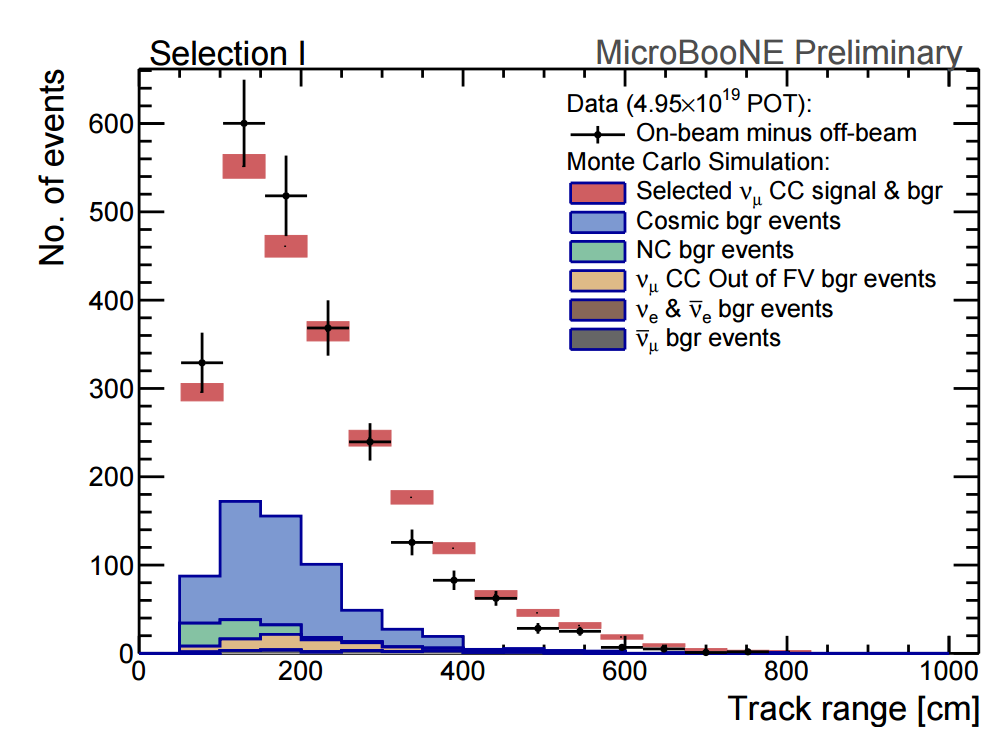
\includegraphics[width=\textwidth]{figs/track_distribution.png}
	\caption{Track range distribution of selection I}
	\label{fig:track}
	\end{subfigure}
	\quad	
	\begin{subfigure}[b]{.4\textwidth}
	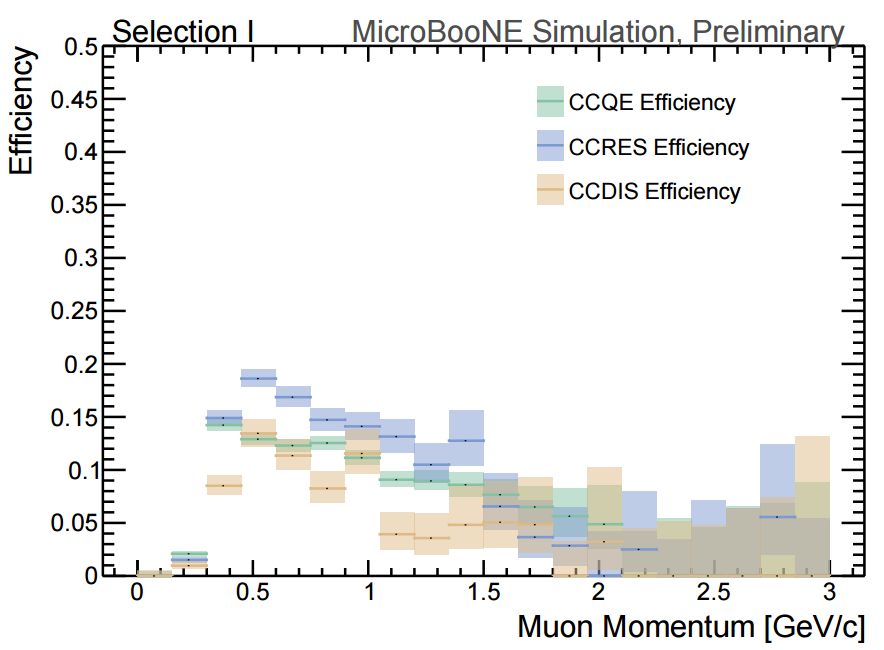
\includegraphics[width=\textwidth]{figs/efficiencyvsmom.png}
	\caption{Selection efficiency as a function of the true muon momentum}
	\label{fig:eff}
	\end{subfigure}
	\quad
\label{fig:distributions}
\caption{\ref{fig:track} Track range distribution for selection I. The track range is defined as the 3D distance between the start and end of the muon candidate track. No data is shown below 75 cm due to the track length cut described previously. \ref{fig:eff} Efficiency of the selected events by process quasi-elastic (QE), resonant (RES), and deep-inelastic (DIS). Statistical uncertainty is shown in the bands and the distributions are a function of true muon momentum. The rise of the efficiency between 0 GeV and 0.5 GeV is due to the minimum track length cut and the decreasing efficiency for higher momentum tracks is caused by the containment requirement.} 
\end{figure}
\section{Optical Software Trigger and Reconstruction}
\subsection{Software Trigger}
Most of the BNB spills from the accelerator do not have a neutrino interaction in MicroBooNE. To save computation resources and reduce data-rates, we require a burst of light in the light collection system in coincidence with the 1.6 $\micro s $ beam spill. Requiring light activity in coincidence with the beam spill eliminates the vast majority of triggers with no neutrino interaction in the detector, however, it doesn't guarantee the activity in the detector is a neutrino interaction since a cosmic ray can interact in coincidence with the beam spill as well.

To implement this, a software trigger was used on the PMT waveforms to decide whether or not to keep that event. The software trigger is implemented after the event builder combines data from the PMTs and triggers into a single event. The software trigger uses the digitized output of the 32 PMT channels in the light collection system. Only the waveform region in coincidence with the beam spill is used to search for possible triggers. For each PMT, a waveform is found by taking the difference of ADC values is calculated between \textit{t} and \textit{t + s}. This waveform is then scanned for ADC values above a threshold \textit{$X_0$}. Once an ADC is above this threshold, a discriminator window is opened for a fixed number of time ticks \textit{($W_0$)}. If the ADC count within this window \textit{$W_0$} is greater than a second larger threshold \textit{$X_3$}, a final window of width \textit{$W_3$} is opened. The max ADC value within this final window is set as the peak amplitude for the PMT and then summed across all 32 PMTs and set to the variable PHMAX. The software trigger places a final cut on the PHMAX variable to decide whether or not to keep the event. The thresholds were found by the Trigger task force using Monte Carlo Studies 
and are as follows: 
\begin{itemize}
\item{$X_0$ = 5 ADC} 
\item{$X_3$ = 10 ADC} 
\item{$W_0$ = 6 Ticks} 
\item{$W_3$ = 6 Ticks} 
\item{PHMAX cut = 130 ADC}
\end{itemize}

\subsection{Flash Reconstruction}
MicroBooNE collects light from each of the 32 PMTs either in a continuous readout window of 23.4 $\micro S$ activated by a beam gate signal on the trigger board, or in discriminated pulses of \sim 1 $\micro s$ duration activated if the ADC count for any PMT goes above 80 ADC count. These two formats are saved as output waveforms and put onto an event. Additionally, each PMT can provide two output streams, high-gain (\sim 20 ADC/PE) and low-gain (\sim 2 ADC/PE) channels. The first step in the reconstruction is to merge both these channels into a ``saturation corrected waveform'' which uses information from the low-gain waveform to correct for saturating high-gain pulses.
 
The saturation corrected waveform in the continuous readout window is used to reconstruct optical hits. Each PMT's waveform is scanned for hits then a threshold based hit reconstruction algorithm is applied which requires pulses of a minimum area in order to be reconstructed. Each reconstructed hit is associated to a PMT, a time in $\micro s$, and a PE count. 

Once hits are reconstructed for all 32 PMTs, all PMT information is then combined into optical flashes which represent optical information seen by the PMTs from interactions in the detector. Each flash has information on total light seen per interaction,  the distribution of the light across all 32 PMTs, the flash time with respect to the trigger time of the flash, and lastly, the spacial information of the flash in Y-Z plane of the detector. These flashes are reconstructed by requiring that there is a \sim 1 $\micro s$ coincidence between the reconstructed hits in all 32 PMTs. The total PE is summed up among all coincident hits across the PMTs and if the total PE is greater than 2 PE, a flash is reconstructed. There are also safe guards in place to take care of late scintillation light.  

\begin{figure}[htp!]
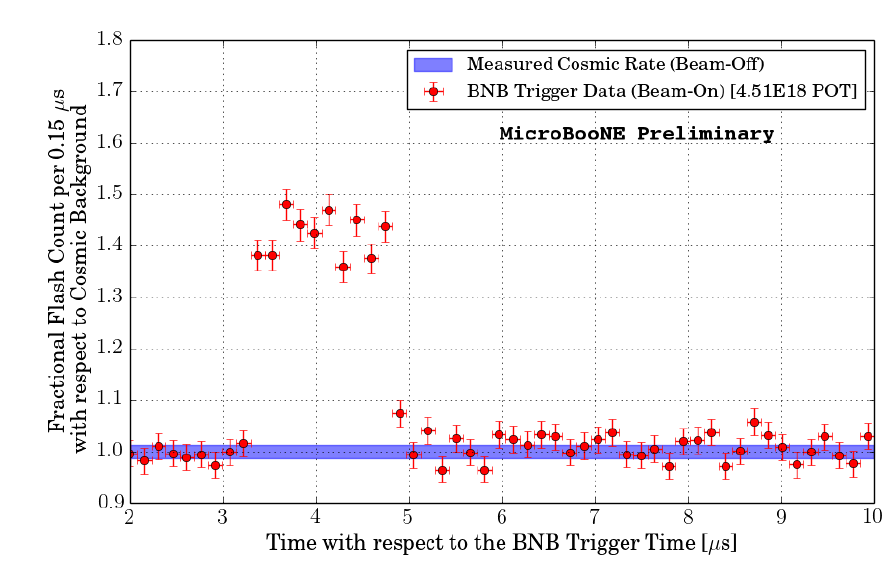
\includegraphics[width=.6\textwidth]{figs/opticaltrigger.png}
\caption{Time distribution of reconstructed optical flashes with a PE value of 50 or more for a sample of BNB unbiased triggered events.}
\label{fig:optrig}
\end{figure}

Figure \ref{fig:optrig} shows the time distribution of reconstructed optical flashes using the BNB continuous stream. You can see a clear excess in coincidence with the expected arrival time of neutrinos. The same flash reconstruction that was used in the cc-inclusive filter detailed here was used to create this plot in data.
\subsection{Beam Window}

\begin{figure}[htp!]
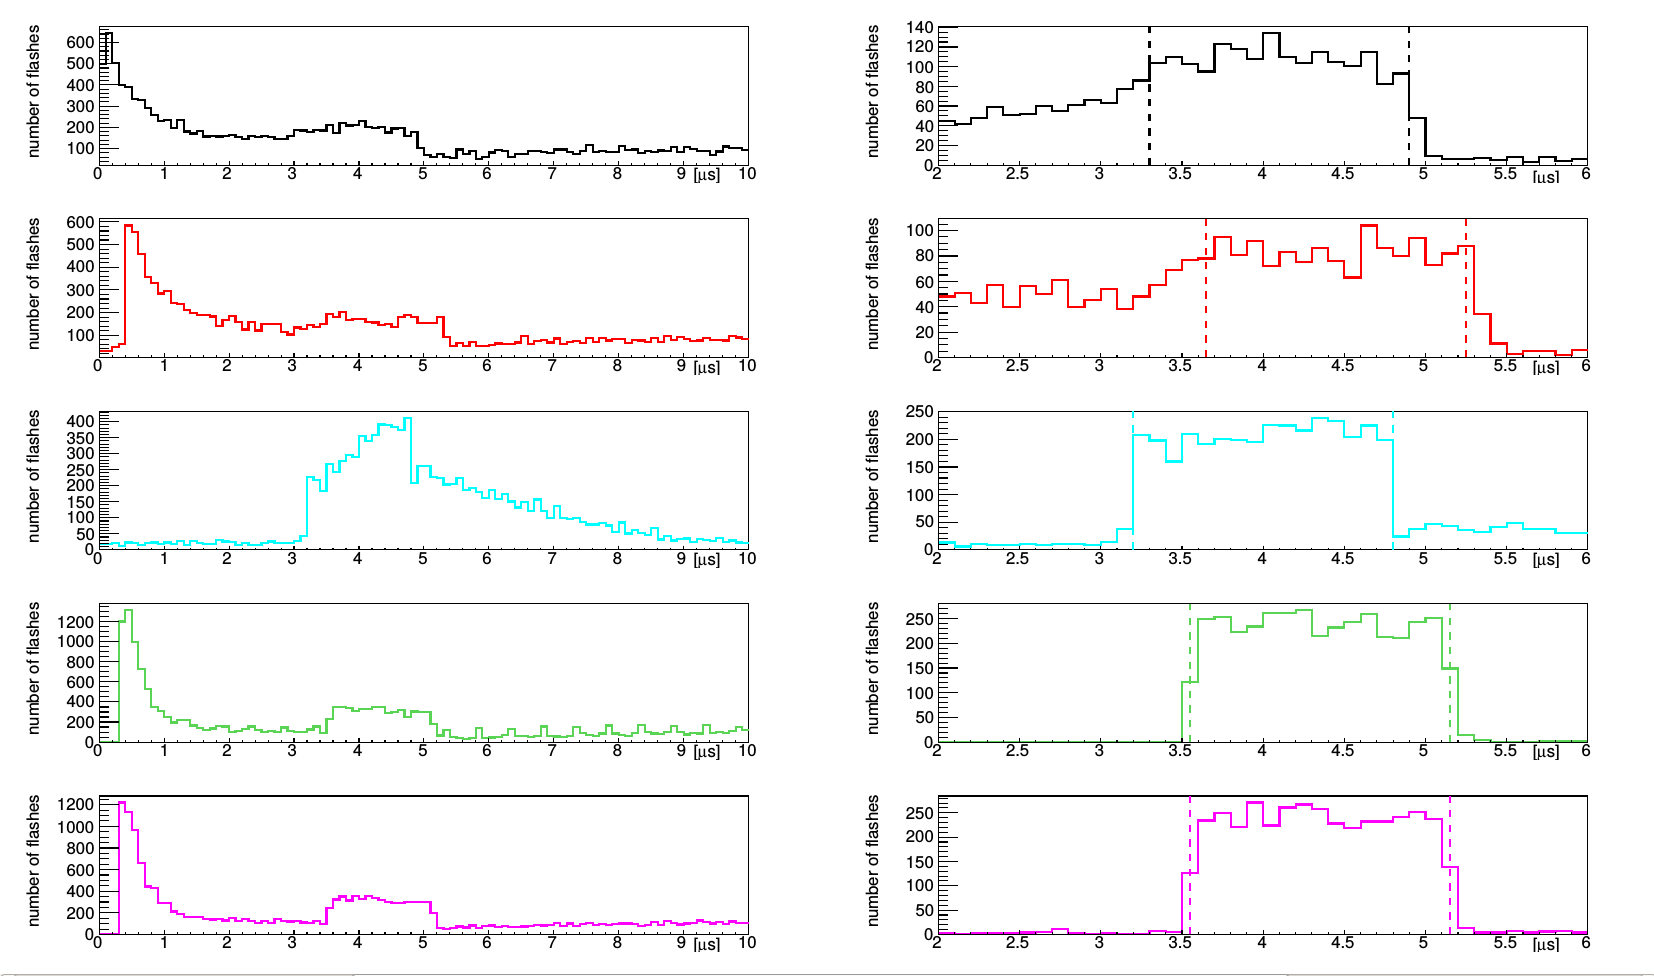
\includegraphics[width=\textwidth]{figs/flashdist.png}
\caption{Flash time distribution for all flashes (left plot) and flashes > 20PE (right plot). The different curves are as follows: on-beam data (black), off-beam data (red), CORSIKA inTime MC (light blue), BNB only MC (green), and BNB+Cosmic MC (purple). The dashed vertical lines mark the time window that was chosen for each sample}
\label{fig:beamwindow}
\end{figure}

Figure \ref{fig:beamwindow} shows the distribution of flashes for on-beam, off-beam and various MC samples. The software trigger has been applied to these samples. The pile-up seen just after 0 $\micro s$ is a feature of the flash finding algorithm and consists of low PE flashes and is removed in the second column of distributions with a low 20 PE threshold cut. The plots show that the time window for the distributions are shifted a small amount from each-other. This is caused by different hardware configurations per sample. Using these distributions, the windows chosen per sample are as follows:
\begin{itemize}
\item{On-Beam: 3.3 to 4.9 $\micro s$}
\item{Off-Beam: 3.65 to 5.25 $\micro s$} 
\item{CORSIKA inTime: 3.2 to 4.8 $\micro s$}
\item{BNB only: 3.55 to 5.15 $\micro s$} 
\item{BNB+Cosmic: 3.55 to 5.15 $\micro s$} 
\end{itemize}
Each window has a width of 1.6 $\micro s$. 


\section{TPC Reconstruction}
\begin{figure}[htp!]
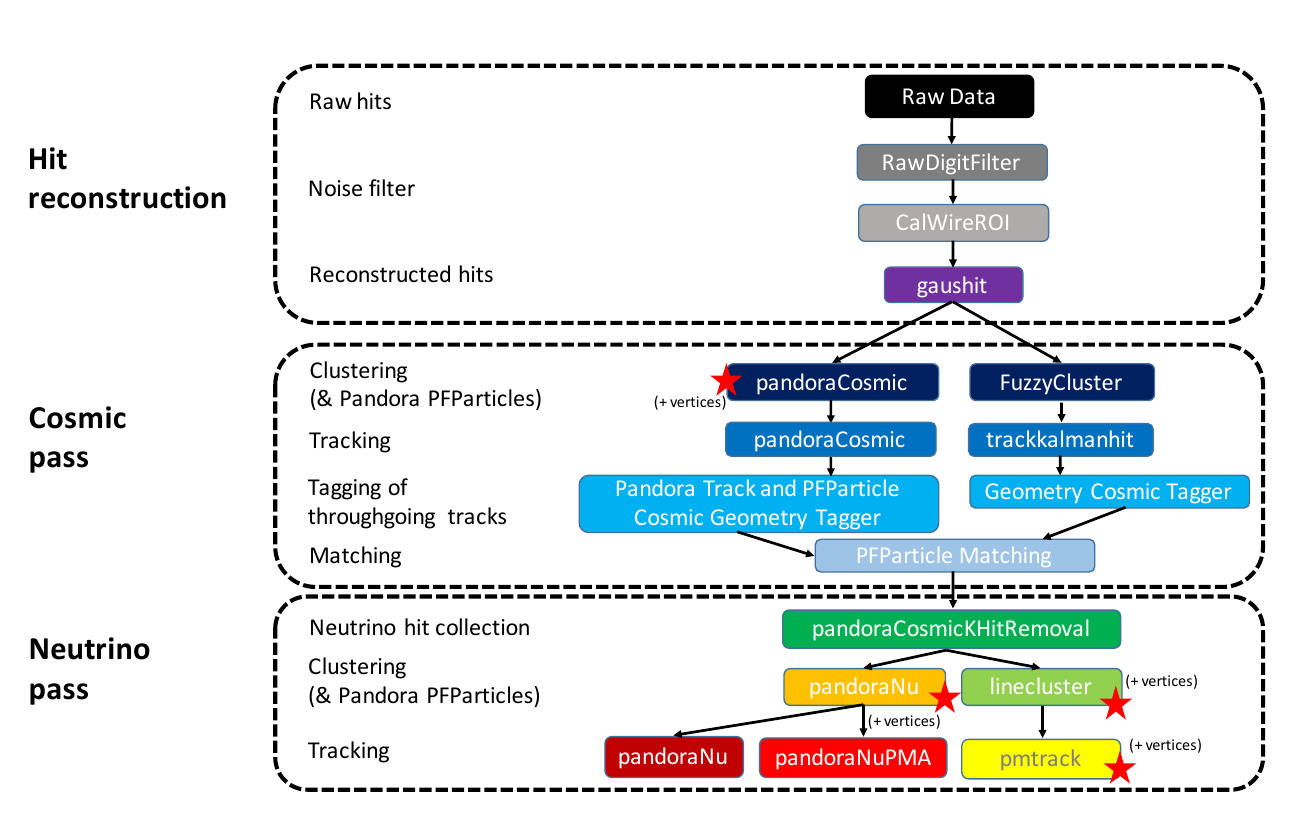
\includegraphics[width=\textwidth]{figs/reconstructionchain.png}
\caption{Reconstruction chain run on both data and MC. The red stars mean that the algorithm returns reconstrucded 3D vertices.}
\label{fig:recochain}
\end{figure}

Figure \ref{fig:recochain} summarizes the reconstruction chain applied to both MC and data for this analysis. After the hit reconstruction, a cosmic pass is applied which removes all hits associated to through-going tracks. A description of these TPC reconstruction algorithms will be detailed below.
\subsection{Hit Reconstruction}
\subsection{Clustering}
\subsection{Pandora}
\subsection{Trackkalmanhit}
\subsection{Cosmic Hit Removal}
\subsection{Projection Matching Algorithm}
\subsection{Calorimetry}
\section{Event Selection}
%\section{The importance of $\mu/\pi$ separation}

  %\chapter{The importance of $\mu/\pi$ separation in MicroBooNE}
$\mu/\pi$ separation chapter goes here.

\clearpage

More $\mu/\pi$ separation.

  \chapter{Convolutional Neural Networks}
Image processing is processing of images by using any form of signal processing. Most image processing techniques treat an image like a 2-dimensional signal and apply standard signal processing techniques to it. Examples of image processing include Gaussian smoothing, edge detection, contouring and pattern recognition or high-level image processing like computer vision. By transforming each sample value for a single wire into a pixel value, it is possible to create an 2-D image from each LArTPC anode plane and hence apply image processing techniques. Gaussian smoothing is used to reduce the noise in an image. Edge detection algorithms look for discontinuities in an image and is the fundamental stage in pattern recognition or any higher level image processing, machine learning and computer vision due to the fact that it extracts the important features in an image. Once edge detection is applied to an image, a contouring algorithm can then be applied. A contour in image processing is an outline bounding an object of interest. A contour must be a closed line outlining in this case the edges found during edge detection. Once we have a bounded object, it is then possible to use these extracted features to train a computer vision algorithm like a Convolutional Neural Network (CNN) to learn that these features describe certain objects, and to then use these computer vision algorithms on random images.


\begin{figure}[t!]
\centering
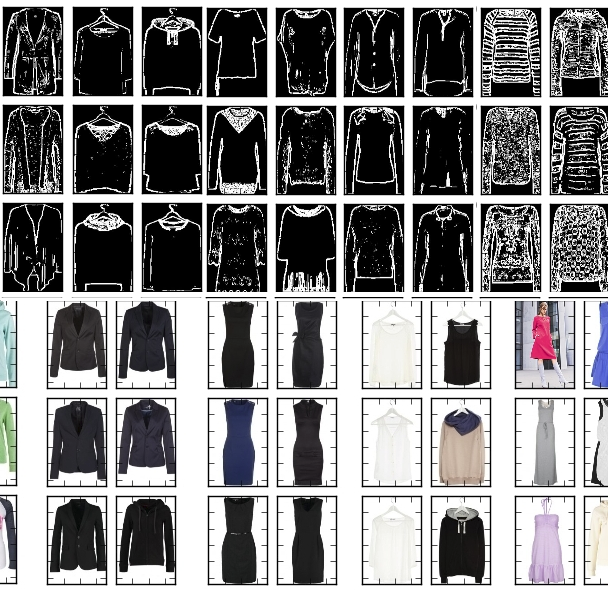
\includegraphics[width=.48\linewidth]{figs/convolution.png}
\caption{Applying a feature mask over a set of fashion items to extract necessary information for auto-encoding. Unnecessary information for example color or brand emblems are not saved. This feature map is an edge detection mask that leaves only shape information which helps to distinguish between different types of clothes.} 
\label{fig:convolution}
\end{figure}


When used for image recognition, convolutional neural networks consist of multiple layers of feature maps that extract different information on small portions of the input image. How many layers and feature maps is tunable to increase the matching process. The output of these collections are then tiled so that they overlap to gain a better representation of the original image and allow for translation. To truly understand CNNs, a breakdown of what convolution means with regards to imaging is necessary. Convolution of an image is using a map of some sort to extract features from the input image by matrix multiplication. The map is multiplied to a small image patch and this is then saved. This is done until the whole image is processed and what is left is a feature map that has the important features extracted. An example of convolution for the process of object identification is shown in figure \ref{fig:convolution}. In this figure you can see how an edge detection feature map is used to save only necessary information for recognizing different types of clothes. You can also see by having multiple feature maps you can get more detail or less detail from an image which can then simplify or complicate the object recognition task. Being able to distinguish between a shirt or a leg garment is as much information you want, having a feature map that extracts outline edge or shape information would be all that you need. But if instead you wanted to distinguish between a formal cocktail dress or a summer dress, more information would need to be saved equating to many more feature maps for one image. Rather than trying to come up with a scheme of feature maps to run over the image by hand, CNNs do this automatically. CNNs take input parameters, for example number of layers, number of units per layers, number of connections per unit, and uses these to create the feature maps. The layers build upon each-other, for example if we were creating a CNN for facial recognition the convolutional layers will start learning feature combinations off of the previous layers. The simple edges, gradients, and corners of the first layers become things like eyes, noses, and hairs in later layers. This process is visualized in figure \ref{fig:featuremaps} 

\begin{figure}[h!]
\centering
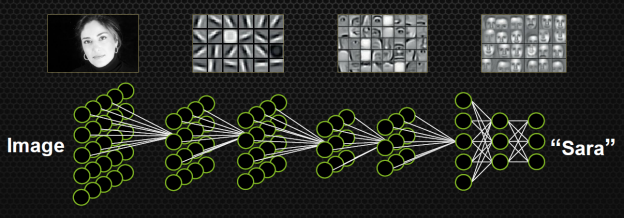
\includegraphics[width=.9\linewidth]{figs/facialDetection.png}
\caption{Pictorial Representation of Convolutional Neural Networks as well as a visual representation on CNN's complexity of layer feature extraction}
\label{fig:featuremaps}
\end{figure}

  %\chapter{Hardware Frameworks}\label{ch:hardware}
Chapter about different frameworks used/timing on each setup.
\section{Syracuse CPU Machine setup}
\section{Syracuse University GPU Cluster Setup}
\dots

  \chapter{Training process of Convolutional Neural Networks}\label{ch:cnn_train}
Three CNNs were trained throughout this analysis. There are differences to each CNN that will be described fully in the next sections but the main difference is the amount of particle images used for training and validation. CNN1075 used 1,075 muons and 1,075 charged pions for training and the same amount of each particle for validation. CNN10000 used 10,000 muons and 10,000 charged pions split in half for testing and training. Lastly CNN100000 had muons, charged pions, protons, electrons, and gammas in its training and validation set. Each particle had 20,000 images and training and validation was split $90\%$ training, $10\%$ validation. This chapter will also describe the different hardware frameworks used for training beginning on a CPU and ending on a GPU cluster. 


%\section{Hardware Frameworks used for Training}
%\subsection{Syracuse CPU Machine setup}
%\subsection{Syracuse University GPU Cluster Setup}


\section{Hardware Configurations for Convolutional Neural Network Training}\label{research approach}
The first training iteration, CNN1075, was a proof of concept. This CNN was trained on my local machine for \sim 4-5 weeks. The batch size had to be very small as well as the image size due to the lack of computation resources. The second iteration of training, CNN10000, was trained on a Fermilab stationed Syracuse University machine. This machine had 6 TB of disk space, 6 cores at 2.1 GHz and 32 GB of RAM. The use of this machine allowed me to increase the training sample as well as the batch size and hence further increase the accuracy of the neural network. Lastly, the CNN100000 was trained using two GTX 1080 Ti GPUs with 11GB of memory on a node on the Syracuse University GPU cluster, SUrge, that has 8 cores and 16GB of memory. This increase in memory as well as the capability to use 2 GPUs drastically cut down on training time from \sim 4-5 weeks to \sim 8 hours. SUrge also allowed for hyperparameter optimization by being able to run multiple training iterations over the two GPUs. Lastly, SUrge allowed for training over higher resolution images and a larger particle class of 5 particles vs 2 particles. 

\section{Creating images using LArTPC data for training/validation of CNNS}\label{image_making}
The $\mu/\pi$ image dataset used to train and validate CNN1075 was created using single generated isotropic muons and charged pions from 0-2 GeV energy range. 2,150 muons and 2,150 charged pions were used for training and testing split 50\%. The images were created using LArSoft, a liquid argon software, and were based on wire number and time tick in the collection plane. Uboonecode reconstruction version v05{\_}08{\_}00 was used. The raw ADC value after noise filtering was the wire signal. Each collection plane greyscale image was 3456x1600x1 where 6 time ticks were pooled into 1 bin. 

After the image was created, the region of interest (ROI) in the image was found by using Open CV, a image processing open source software package, to scan the image starting from the edges and stopping once a bright pixel is encountered. At this step, the ROI can be larger or smaller than the necessary size of a training image and the XY ratio of the image is not kept. This ROI is then resized to an image of 224x224x1. 

The greyscale color standard is 8bit therefore the ADC value of wire and time tick was also downsampled due to the 12bit MicroBooNE ADC value. To do this, the highest ADC pixel in the image was found and then this was divided by the rest placing all pixel values between 0-1. From there, all pixel values are then multiplied by 255.

The $\mu/\pi$ image dataset used to train and validate the CNN10000 was also created using single generated isotropic muons and charged pions from 0-2 GeV energy range. 10,000 muons and 10,000 charged pions were used for training and testing split 50\%. Uboonecode v06{\_}23{\_}00 was used instead of v05{\_}08{\_}00. Each collection plane greyscale image was 3456x1280x1 where 5 time ticks were pooled into 1 bin which is different than the previous dataset and was implemented due to the fact that the time ticks of an event went from 9400 to 6400 with the change of uboonecode version. Issues that arose in CNN1075 that were fixed in CNN10000 include zero-padding images in X and Y that are smaller than 224X224 to eliminate over-zooming effect and fixing a bug that shifted pixels separated by a dead-wire region.

The $\mu/\pi/p/e/\gamma$ image dataset used to train and validate the CNN100000 were created using single generated isotropic particles with energy range from 0-2 GeV. 20,000 of each particle were used for training and were split 90/10 between training and testing sets. Uboonecode v06{\_}23{\_}00 was used for these images. The collection plane greyscale image had the same dimensions as CNN10000, 3456x1280x1 and the ROI algorithm was the same except for resizing these images to 576x576. 

A major change other than the higher resolution images was the treatment of the ADC values. In the first two image making schemes, the highest pixel value was found per image and the image was then normalized by that. The issue arising from this ADC normalization wasn't inherent in $\mu/\pi$ training due to the fact that both particles are minimum ionizing particles in liquid argon, however, when dealing with a larger particle class, it was necessary to try and make sure energy deposition by each particle was preserved. The energy deposition in a particle image corresponds to the ADC value or pixel brightness. To preserve energy deposition, the ADC float value was passed straight to the image rather than doing any image normalization. This then makes sure that minimum ionizing particles like muons and charged pions appear dimmer than highly ionizing particles like protons.  

Images were also made from BNB+Cosmic events that passed the cc-inclusive selection 1 filter right before the 75 cm track length cut and were classified using the CNN10000. The dataset used to create these images is the same one used in \cite{cc-inclusive}, \textit{prodgenie{\_}bnb{\_}nu{\_}cosmic{\_}uboone{\_}mcc7{\_}reco2}. These images were created using information from the track candidate that passed the filter. Only wire number and time ticks associated to the track candidate were drawn on the image to mimic a single particle generated image. 

These images were then classified using CNN10000. Two approaches were taken in making these images. The first was using the image normalization above where the maximum pixel in each image is used as a normalization constant to get all pixels between 0-1 then multiply all pixels by 255. As described above, this is the incorrect way to normalize. The second way the images were created was by passing the ADC float to the image. 

Lastly, multiple BNB+Cosmic images per event were made for CNN100000 by reducing many of selection I cuts to try and let the CNN do particle as well as event identification. This image making scheme used for CNN100000 will be described in more detail in later sections. 

\section{Convolutional Neural Network Training}
\subsection{Training CNN1075}
The results of CNN1075 are described in this section. The accuracy is how well CNN1075 is doing by epoch and was 74.5\%. The loss is gradient descent or minimization of the error of the weights and biases used in each neuron of each layer of CNN1075 and was 58\% with a trend sloping downwards on the loss curve as well as a trend sloping upward in the accuracy curve. The accuracy and loss of CNN1075 are shown in figure \ref{fig:loss_accuracy_1075}. Due to the depth of the neural network framework, it was necessary to train with a larger dataset and for more epochs, however, the downward slope of the loss curve is an indication that once trained for longer with a higher training sample, neural networks can be used for $\mu/\pi$ separation. The hyperparameters used to train CNN1075 are detailed below: 

\begin{multicols}{3}
\begin{itemize}
 \item \textit{train{\_}batch{\_}size: 50}
 \item \textit{test{\_}batch{\_}size: 50}
 \item \textit{test{\_}iter: 50}
 \item \textit{test{\_}interval: 50}
 \item \textit{base{\_}lr: 0.01}
 \item \textit{lr{\_}policy: "step"}
 \item \textit{gamma: 0.1}
 \item \textit{stepsize: 200}
 \item \textit{display: 50}
 \item \textit{max{\_}iter: 5000}
 \item \textit{momentum: 0.9}
 \item \textit{weight{\_}decay: 0.0005}
 \item \textit{snapshot: 100}
\end{itemize}
\end{multicols}

\begin{figure}[htp!]
\centering
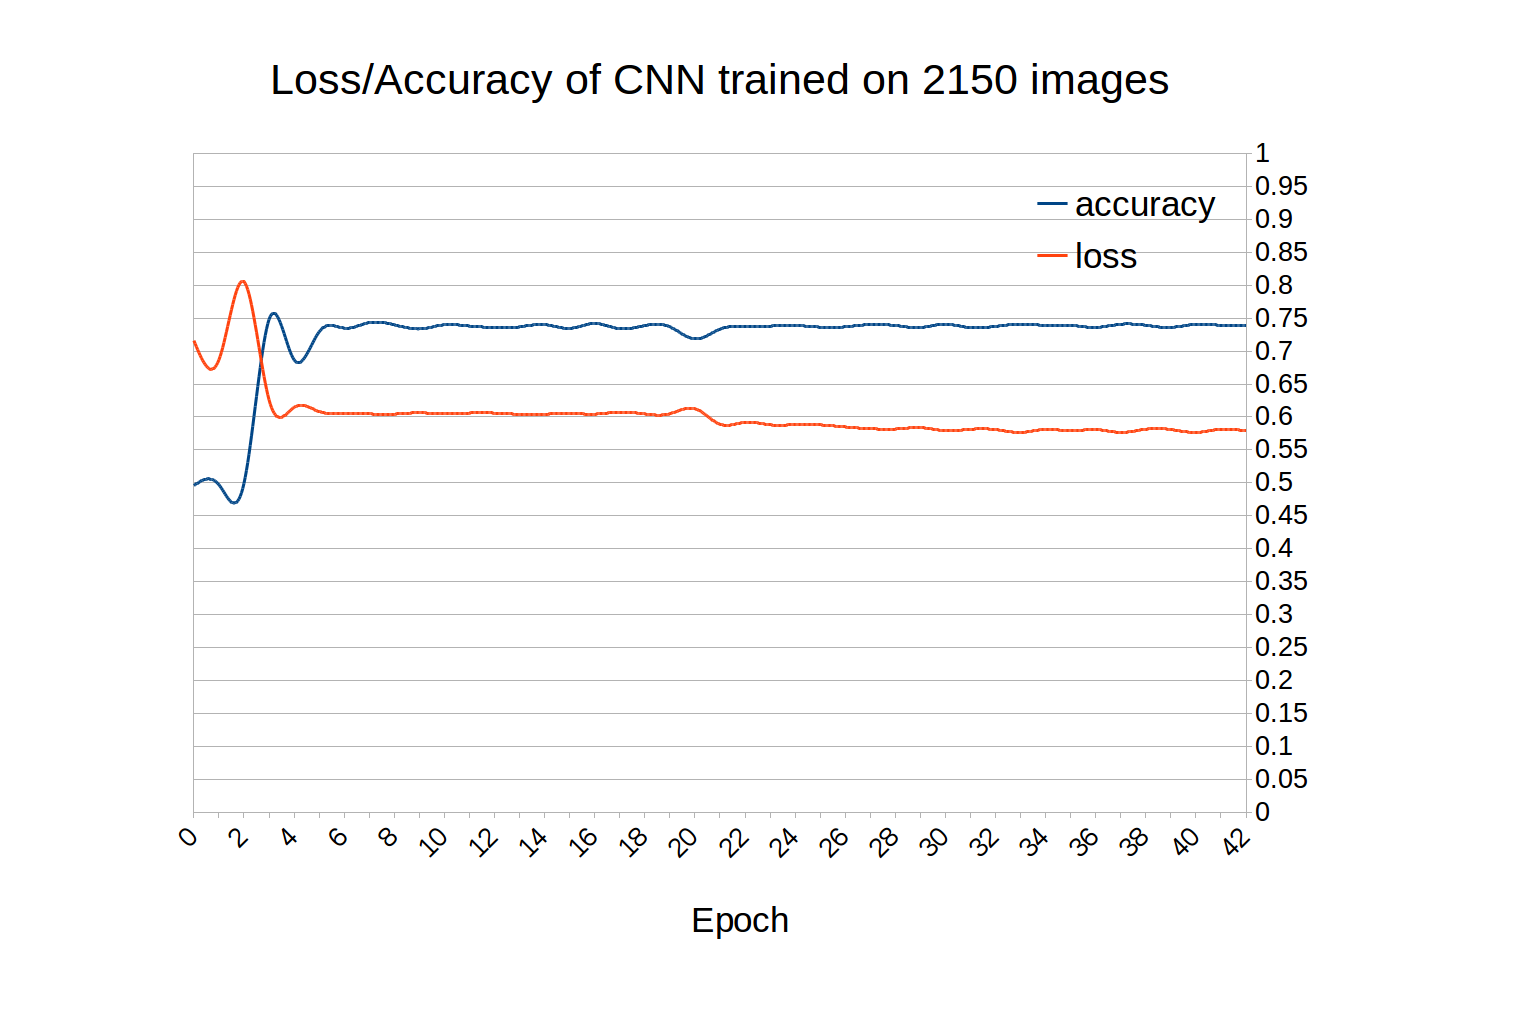
\includegraphics[width=\textwidth]{figs/acc_loss_CNN1075.png}
\caption{Accuracy vs. Loss of AlexNet 2-output $\mu/\pi$ sample consisting of 2,150 images each.} 
\label{fig:loss_accuracy_1075}
\end{figure}


\begin{figure}[htp!]
\centering
	\begin{subfigure}[b]{.68\textwidth}
	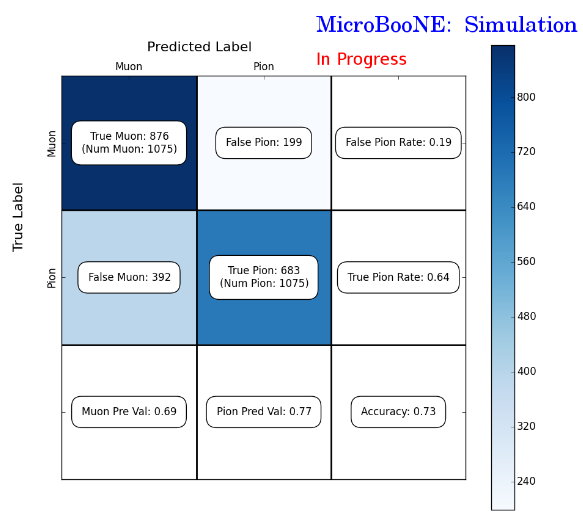
\includegraphics[width=\textwidth,height=3in]{figs/confusion1_train.png}
	\caption{Confusion Matrix showing Accuracy of CNN1075 using training MC data}
	\end{subfigure}
	\quad
	\begin{subfigure}[b]{.6\textwidth}
	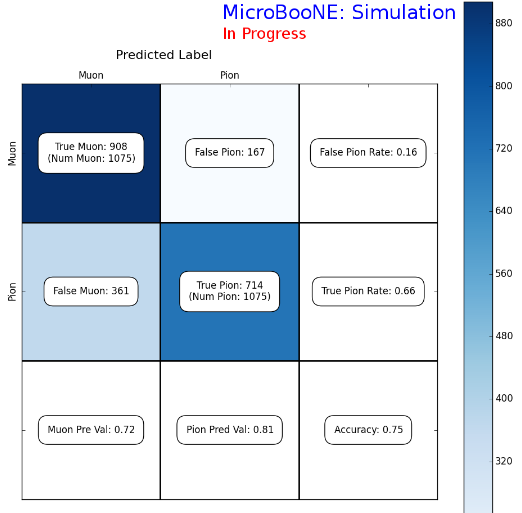
\includegraphics[width=\textwidth,height=3in]{figs/confusion1_test.png}
	\caption{Confusion Matrix showing Accuracy of CNN1075 using testing MC data}
	\end{subfigure}
	\quad
\caption{Description of confusion matrix variables: False pion rate = $false \pi/ total \pi$ True pion rate = $true \pi/total \pi$ Accuracy = $(true \pi rate + true \mu rate)/2$ Pion prediction value = $true \pi/(true \pi + false \pi)$ Muon prediction value = $true \mu/(true \mu + false \mu)$}
\label{fig:confusion1075}
\end{figure}

The confusion matrices shown in figure \ref{fig:confusion1075} show the accuracy for both the training and testing datasets. The fact that these two have similar accuracies is important because if the training dataset had a much higher accuracy, that indicates an over-training of the training sample which means the neural network didn't learn features to separate muons from charged pions, it just memorized what was in the training dataset. Also note that the neural network does a better job of identifying muons than charged pions. This can be attributed to the more complex event scenes charged pions tend to leave in the detector due to pion interacting more in LAr than muons do. The CNN may do better at identifying charged pions with a larger training sample.

\subsection{Training CNN10000}
The hyperparameters used for CNN10000 are shown below. The batch size for the training and testing as well as the test{\_}iter were chosen to encompass the whole training/testing image set when doing accuracy/loss calculations. To do this, multiplying the test{\_}iter by the test batch size gives you the amount of images used when calculating accuracy/loss curves. 

\begin{multicols}{3}
\begin{itemize}
 \item \textit{train{\_}batch{\_}size: 100}
 \item \textit{test{\_}batch{\_}size: 100}
 \item \textit{test{\_}iter: 100}
 \item \textit{test{\_}interval: 100}
 \item \textit{base{\_}lr: 0.001}
 \item \textit{lr{\_}policy: "step"}
 \item \textit{gamma: 0.1}
 \item \textit{stepsize: 1000}
 \item \textit{display: 100}
 \item \textit{max{\_}iter: 10000}
 \item \textit{momentum: 0.99}
 \item \textit{weight{\_}decay: 0.0005}
 \item \textit{snapshot: 100}
\end{itemize}
\end{multicols}

\begin{figure}[htp!]
\centering
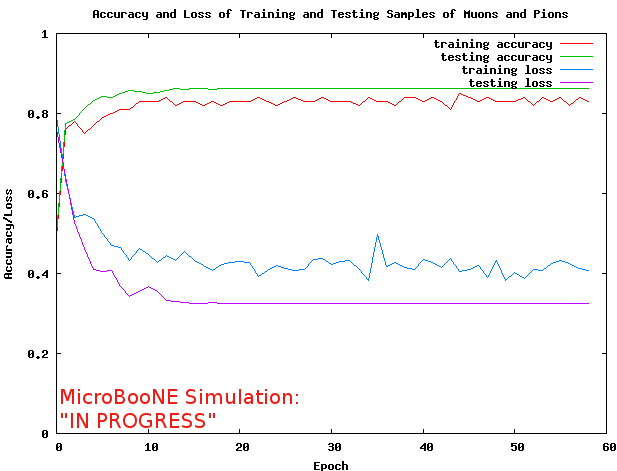
\includegraphics[width=\textwidth]{figs/acc_loss_10000_062117.png}
\caption{Accuracy vs. Loss of AlexNet 2-output $\mu/\pi$ sample consisting of 10,000 images each.} 
\label{fig:loss_accuracy}
\end{figure}

The same architecture that was used to train CNN1075 was employed on CNN10000, AlexNet. Caffe \cite{caffe} was the software package used for both CNNs. The differences include batch size and test{\_}iter and momentum to account for the larger dataset. Figure \ref{fig:loss_accuracy} shows the loss and accuracy of CNN10000. There is around a 10\% increase in accuracy from CNN1075 to CNN10000, 85\%, and around a 20\% decrease in loss, 36\%.

\begin{figure}[htp!]
\centering
	\begin{subfigure}[b]{.7\textwidth}
	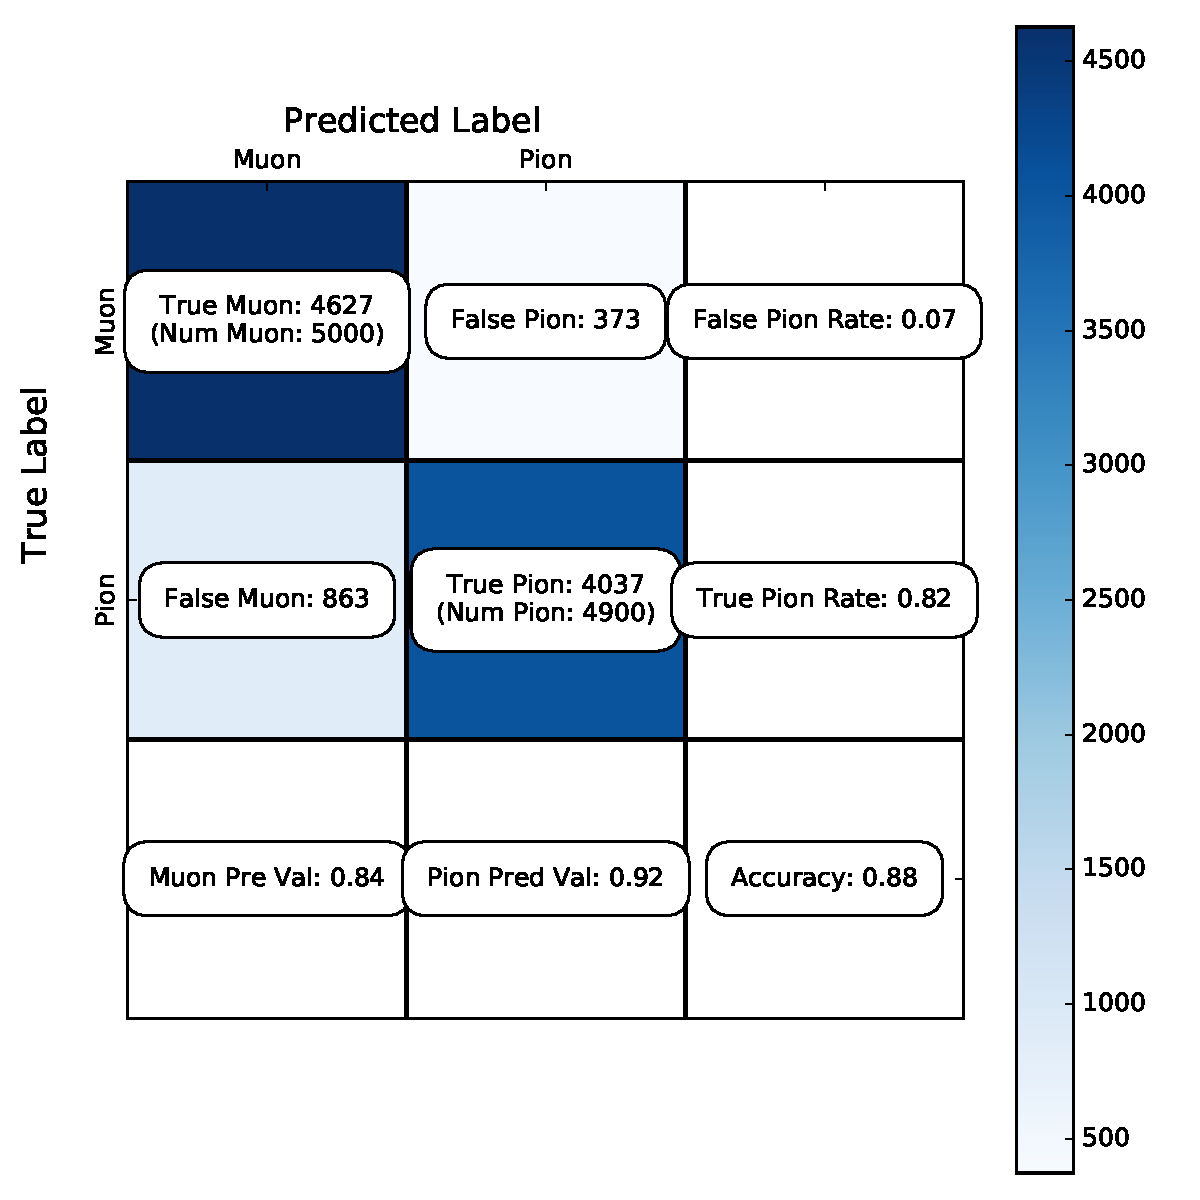
\includegraphics[width=\textwidth,height=3.5in]{figs/train_confusion.pdf}
	\caption{Confusion Matrix showing Accuracy of CNN10000 using training MC data}
	\label{fig:confusion}
	\end{subfigure}
	\quad
	\begin{subfigure}[b]{.7\textwidth}
	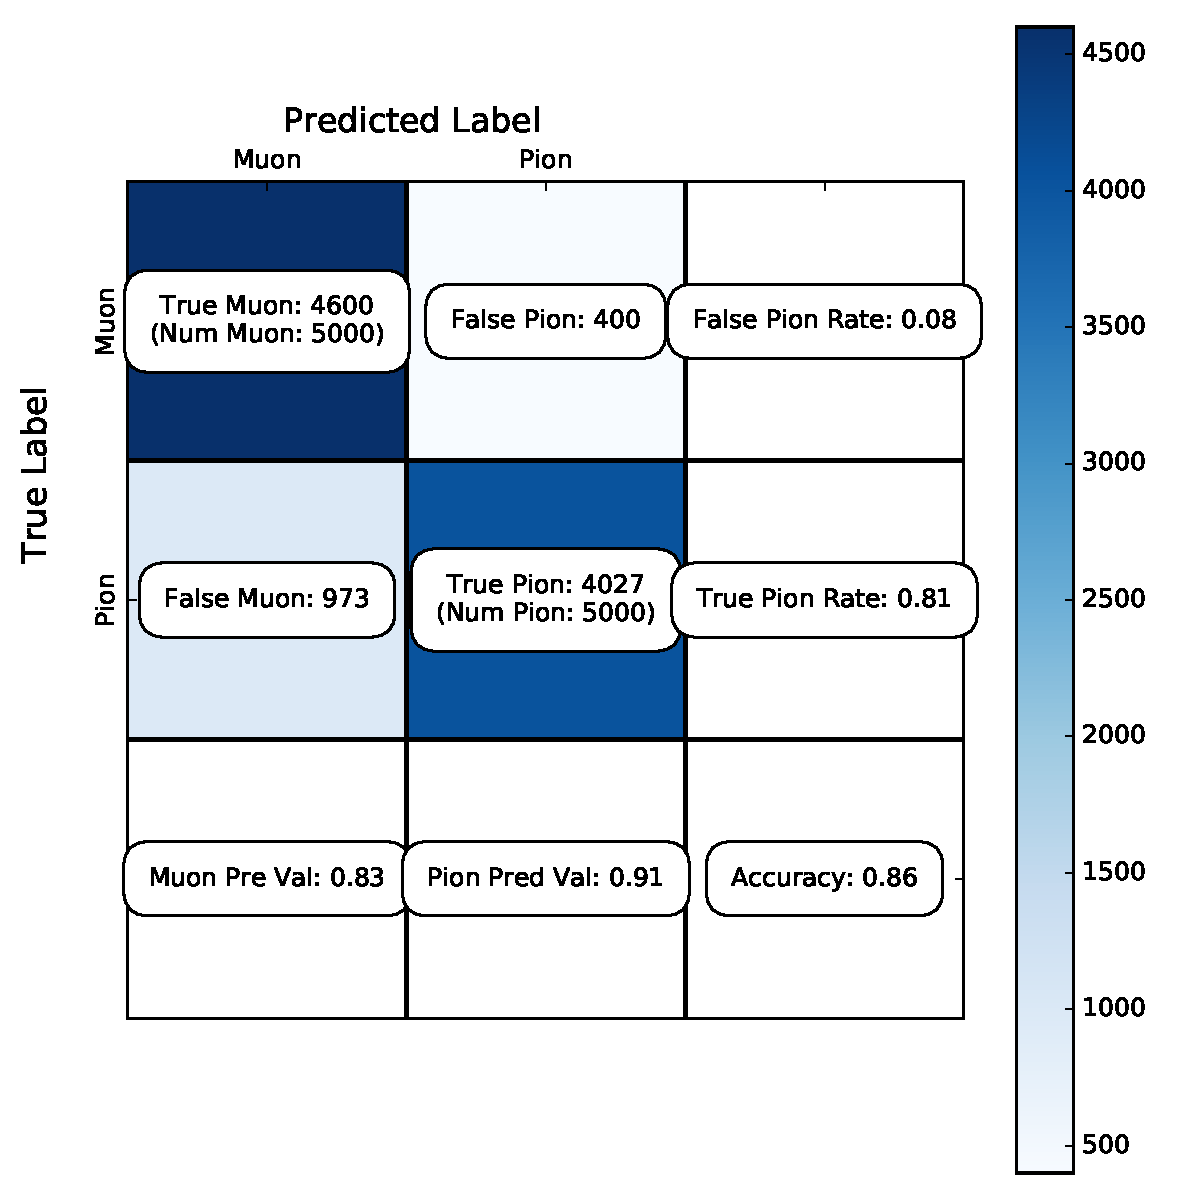
\includegraphics[width=\textwidth,height=3.5in]{figs/val_confusion.pdf}
	\caption{Confusion Matrix showing Accuracy of CNN10000 using testing MC data}
	\label{fig:confusion_test}
	\end{subfigure}
	\quad
\caption{Description of confusion matrix variables: False pion rate = $false \pi/ total \pi$; True pion rate = $true \pi/total \pi$; Accuracy = $(true \pi rate + true \mu rate)/2$; Pion prediction value = $true \pi/(true \pi + false \pi)$; Muon prediction value = $true \mu/(true \mu + false \mu)$}
\label{fig:CNN_train}
\end{figure}
\begin{figure}[htp!]
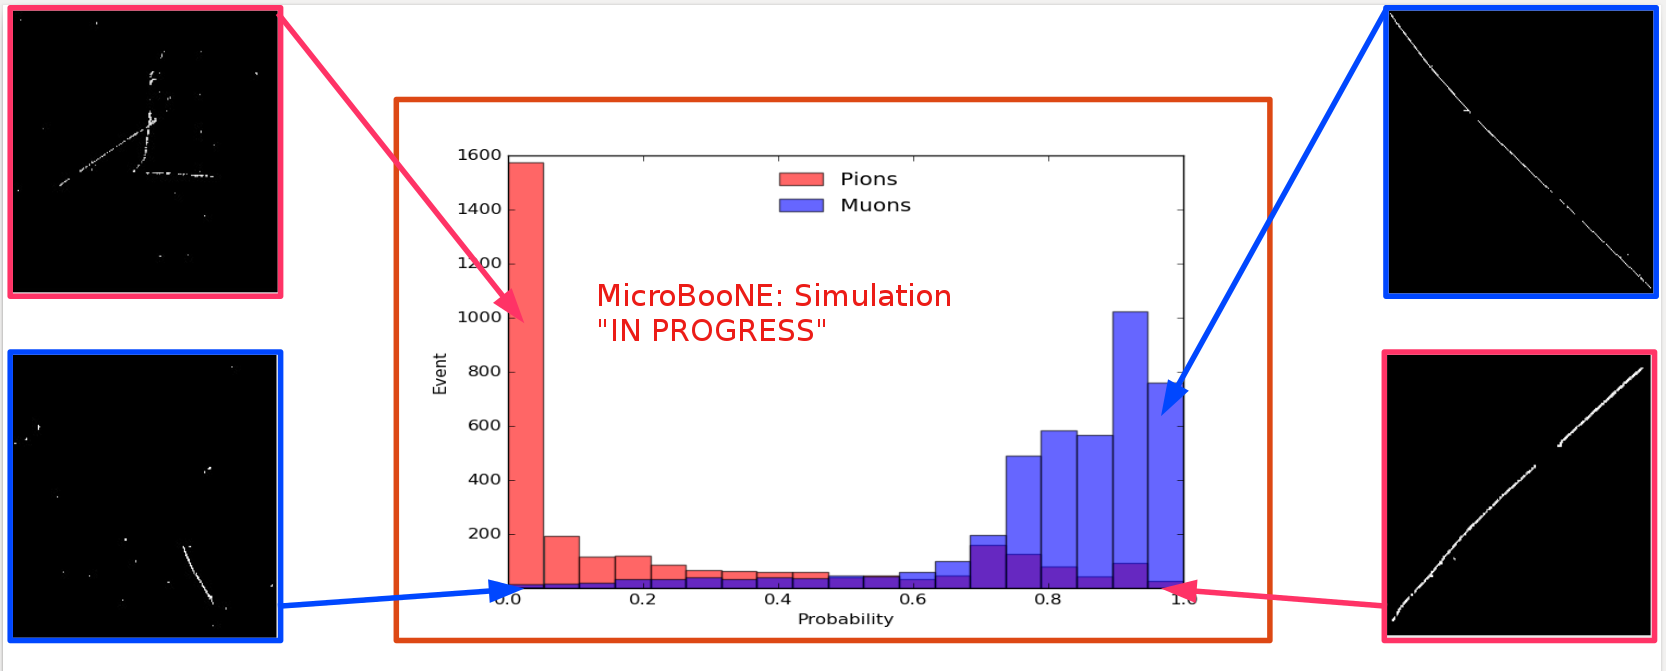
\includegraphics[width=\textwidth]{figs/mitch_hw.png}
\caption{Probability plot of muons and charged pions from testing set. Images surrounding histogram are a random event from lowest bin and highest bin for each particle.}
\label{fig:prob_plot}
\end{figure}

Figure \ref{fig:CNN_train} show a breakdown of $\mu/\pi$ separation for CNN10000. It also shows the network is not being over-trained due to the Accuracy of both the training and testing datasets being within 2\% of each-other. Figure \ref{fig:prob_plot} shows how well the neural network is doing at $\mu/\pi$ separation with respect to muon probability. The red bins corresponds to true charged pions and the blue bins correspond to true muons. There is still pion contamination in the high muon probability bins but by choosing a muon probability of $\geq 80\%$ we can reduce this. The CNNs increase in total accuracy can be attributed to an increase in accurately classifying charged pions as charged pions as seen in both the confusion matrix in figure \ref{fig:CNN_train} and the large number of events in the zero bin of the muon probability plot seen in figure \ref{fig:prob_plot} that corresponds to high probability charged pions.   



\subsection{Training CNN100000}
CNN100000 used the GoogleNet architecture rather than the AlexNet architecture used in the two previous trained CNNs. This is the first time the neural network was trained on a larger particle class, $\mu/\pi/p/\gamma/e$, and on higher resolution images. This CNN also employed GPUs during the training process. The hyperparameters are shown below:

\begin{multicols}{3}
\begin{itemize}
 \item \textit{train{\_}batch{\_}size: 18}
 \item \textit{test{\_}batch{\_}size: 2}
 \item \textit{test{\_}iter: 2000}
 \item \textit{test{\_}interval: 2000}
 \item \textit{base{\_}lr: 0.001}
 \item \textit{lr{\_}policy: "step"}
 \item \textit{gamma: 0.96}
 \item \textit{stepsize: 10000}
 \item \textit{average{\_}loss: 40}
 \item \textit{display: 40}
 \item \textit{max{\_}iter: 10000}
 \item \textit{momentum: 0.99}
 \item \textit{weight{\_}decay: 0.0002}
 \item \textit{snapshot: 50000}
\end{itemize}
\end{multicols}


\begin{figure}[htp!]
\centering
\includegraphics[width=.8\textwidth]{../images/GPU_9010split_hires_iterations_alldata_allparticle.png}
\caption{Training and testing accuracy of CNN trained on 100,000 images of \mu/\pi/p/\gamma/e with 20,000 images of each particle. Each image was a size of 576x576 and the images per particle were split 90\% use for training and 10\% used for testing the network}
\label{fig:gpuacc}
\end{figure}

\begin{figure}[htp!]
\centering
\includegraphics[width=.8\textwidth]{../images/GPU_9010split_hires_iterations_alldata_allparticle_loss.png}
\caption{Training and testing loss of CNN trained on 100,000 images of \mu/\pi/p/\gamma/e}
\label{fig:gpuloss}
\end{figure}
The accuracy and loss for CNN100000 are shown in figures \ref{fig:gpuacc} and \ref{fig:gpuloss}. The jumps shown in both figures are when the training was stopped to fine-tune the weight decay and the learning rate. The accuracy leveled off at \sim 80\% and the loss was at \sim 0.48. 



\begin{figure}[htp!]
\centering
\includegraphics[width=\textwidth]{../images/confusion_allparticle_v3.pdf}
\caption{Confusion Matrix of all five particles }
\label{fig:confusion100000}
\end{figure}
Figure \ref{fig:confusion100000} shows the confusion matrix of CNN100000. The proton identification of the neural network is at 85\% and the highest out of all five particles. One thing to note is clear separation between particles that leave track like objects in the MicroBooNE detector, $\mu/\pi/p$, versus particles that leave shower like objects in MicroBooNE, $e/\gamma$. 



\begin{figure}[htp!]
\centering
\includegraphics[width=.8\textwidth]{../csv_output/true_labels_1102.png}
\caption{t-SNE of CNN}
\label{fig:tsne}
\end{figure}
Another visualization of how the neural network is learning is shown in \ref{fig:tsne}.  t-SNEs \cite{tsne} is a technique used for dimensionality reduction developed for use in visualizing high-dimensional datasets. Each datapoint is given a location in a two or three-dimensional map by using stochastic neighbor embedding to convert high-dimensional euclidean distances between datapoints into conditional probabilities that represent the similarities between these datapoints. For datapoints close together on the map, their conditional probabilities are high, for datapoints with a wide separation between them, their conditional probabilities are very small. Figure \ref{fig:tsne} is a t-SNE of the final training iteration of a subset of the training sample used in CNN100000. You can see a clear separation between track like objects and shower like objects. You can also see that electrons and gammas are not as separated as muons, pions, and protons. For the purpose of this thesis, this isn't an issue but later iterations of training could include more images for the gamma and electron classes to help the CNN further separate these classes. There is also a small cluster of charged pions in close proximity to the muon cluster rather than the large charged pion cluster. This small charged pion cluster still needs to be explored, but a good guess would be that this cluster are of charged pions that have decayed to muons.


\begin{figure}
\centering
	\begin{subfigure}[b]{.475\textwidth}
		\centering
		\includegraphics[width=\textwidth]{../csv_output/muon_prob.png}
		\caption{Muon Prob}
		\label{fig:muonprob}
	\end{subfigure}
	\begin{subfigure}[b]{.475\textwidth}
		\centering
		\includegraphics[width=\textwidth]{../csv_output/pi_prob.png}
		\caption{Pion Prob}
		\label{fig:piprob}
	\end{subfigure}
	\begin{subfigure}[b]{.475\textwidth}
		\centering
		\includegraphics[width=\textwidth]{../csv_output/proton_prob.png}
		\caption{Proton Prob}
		\label{fig:pprob}
	\end{subfigure}
	\begin{subfigure}[b]{.475\textwidth}
		\centering
		\includegraphics[width=\textwidth]{../csv_output/eminus_prob.png}
		\caption{Electron Prob}
		\label{fig:eminusprob}
	\end{subfigure}
	\begin{subfigure}[b]{.475\textwidth}
		\centering
		\includegraphics[width=\textwidth]{../csv_output/gamma_prob.png}
		\caption{Gamma Prob}
		\label{fig:gammaprob}
	\end{subfigure}
\caption{Probabilities of different particle classes as well as their contamination from other classes}
\label{fig:particleprob}
\end{figure}
Figure \ref{fig:particleprob} shows the probability of each particle class and the highest probability misidentification for each class. For muons, the largest misidentification is from protons. For pions, both protons and muons get misidentified as pions at around the same probability. Similar behavior is also seen for proton identification. Electrons and gammas are misidentified as each-other with similar probabilities.  



\begin{figure}[htp]
\centering
\includegraphics[width=.8\linewidth=]{../csv_output/prob_allparticle_normalized.pdf}
\caption{Muon probability of true muons (blue) versus pions (red), protons (cyan), gammas (green) and electrons (magenta).}
\label{fig:prob}
\end{figure}
To see what type of background contamination one would be dealing with when doing muon identification, muon probabilities for each particle class was plotted against the probability of true muons to see how well muon signal vs other particle background separation can be done with CNN100000. Figure \ref{fig:prob} is showing the true muon probability for true muons, versus the rest of the particle classes. This plot describes which muon probability value should be chosen for the least amount of other particle contamination. For electrons and gammas, a muon probability of \sim 75\% would eliminate $e/\gamma$ contamination. For pions and protons, there is contamination at all values of muon probability, but the contamination is drastically reduced at a muon probability $\geq 75\%$, more so for the protons which is so small it's difficult to see on the plot.
 
One of the main concerns with training a neural network was that the features the network would learn to separate muons from charged pions would be track range, which is what was used to begin with in selection I. To make sure that wasn't the case, the next thing that was looked at was the muon probability versus track range and momentum of the track. Figures \ref{fig:mupi_kinematics} through \ref{fig:mug_kinematics} show the muon probability in blue for all plots against all other particles. The point is the average muon probability in that bin and the error bars are the spread of muon probability in that bin. A zoomed in version of track range plot at low track ranges for all particles was also plotted to make sure there is separation between the particles at low track range. The $\mu/\pi$ separation in track range and momentum is less than for $p/e/\gamma$ but that was to be expected. Although the separation isn't as good as the other particles, there still is separation at low momentum and low track range which cannot be done by using a track range cut like selection I does.  
\begin{figure}[htp]
\centering
	\begin{subfigure}[t]{.475\textwidth}
		\centering
		\includegraphics[width=\textwidth]{../csv_output/mu_pi_acc_tracklength_all.pdf}
		\caption{Track range versus muon probability for true muons (blue) and true pions (red).}
		\label{fig:mupi_tracklength}
	\end{subfigure}
	\begin{subfigure}[t]{.475\textwidth}
		\centering
		\includegraphics[width=\textwidth]{../csv_output/mu_pi_acc_tracklength_75.pdf}
		\caption{Track range $\leq 75$ cm versus muon probability for true muons (blue) and true pions (red).}
		\label{fig:mupi_tracklength75}
	\end{subfigure}
	\begin{subfigure}[t]{.475\textwidth}
		\centering
		\includegraphics[width=\textwidth]{../csv_output/mu_pi_acc_momentum.pdf}
		\caption{Momentum versus muon probability for true muons (blue) and true pions (red).}
		\label{fig:mupi_momentum}
	\end{subfigure}
\caption{Kinematic distributions versus muon probability for true muons and true pions.}
\label{fig:mupi_kinematics}
\end{figure}

\begin{figure}[htp]
\centering
	\begin{subfigure}[b]{.475\textwidth}
		\centering
		\includegraphics[width=\textwidth]{../csv_output/mu_p_acc_tracklength_all.pdf}
		\caption{Track range versus muon probability for true muons (blue) and true protons (cyan).}
		\label{fig:mup_tracklength}
	\end{subfigure}
	\begin{subfigure}[b]{.475\textwidth}
		\centering
		\includegraphics[width=\textwidth]{../csv_output/mu_p_acc_tracklength_75.pdf}
		\caption{Track range $\leq 75$ cm versus muon probability for true muons (blue) and true protons (cyan).}
		\label{fig:mup_tracklength75}
	\end{subfigure}
	\begin{subfigure}[b]{.475\textwidth}
		\centering
		\includegraphics[width=\textwidth]{../csv_output/mu_p_acc_momentum.pdf}
		\caption{Momentum versus muon probability for true muons (blue) and true protons (cyan).}
		\label{fig:mup_momentum}
	\end{subfigure}
\caption{Kinematic distributions versus muon probability for true muons and true protons.}
\label{fig:mup_kinematics}
\end{figure}

\begin{figure}[htp]
\centering
	\begin{subfigure}[b]{.475\textwidth}
		\centering
		\includegraphics[width=\textwidth]{../csv_output/mu_e_acc_tracklength_all.pdf}
		\caption{Track range versus muon probability for true muons (blue) and true electrons (magenta).}
		\label{fig:mue_tracklength}
	\end{subfigure}
	\begin{subfigure}[b]{.475\textwidth}
		\centering
		\includegraphics[width=\textwidth]{../csv_output/mu_e_acc_tracklength_75.pdf}
		\caption{Track range $\leq 75$ cm versus muon probability for true muons (blue) and true electrons (magenta).}
		\label{fig:mue_tracklength75}
	\end{subfigure}
	\begin{subfigure}[b]{.475\textwidth}
		\centering
		\includegraphics[width=\textwidth]{../csv_output/mu_e_acc_momentum.pdf}
		\caption{Momentum versus muon probability for true muons (blue) and true electrons (magenta).}
		\label{fig:mue_momentum}
	\end{subfigure}
\caption{Kinematic distributions versus muon probability for true muons and true electrons.}
\label{fig:mue_kinematics}
\end{figure}

\begin{figure}[htp]
\centering
	\begin{subfigure}[b]{.475\textwidth}
		\centering
		\includegraphics[width=\textwidth]{../csv_output/mu_g_acc_tracklength_all.pdf}
		\caption{Track range versus muon probability for true muons (blue) and true gammas (green).}
		\label{fig:mug_tracklength}
	\end{subfigure}
	\begin{subfigure}[b]{.475\textwidth}
		\centering
		\includegraphics[width=\textwidth]{../csv_output/mu_g_acc_tracklength_75.pdf}
		\caption{Track range $\leq 75$ cm versus muon probability for true muons (blue) and true gammas (green).}
		\label{fig:mug_tracklength75}
	\end{subfigure}
	\begin{subfigure}[b]{.475\textwidth}
		\centering
		\includegraphics[width=\textwidth]{../csv_output/mu_g_acc_momentum.pdf}
		\caption{Momentum versus muon probability for true muons (blue) and true gammas (green).}
		\label{fig:mug_momentum}
	\end{subfigure}
\caption{Kinematic distributions versus muon probability for true muons and true gammas.}
\label{fig:mug_kinematics}
\end{figure}



  \chapter{Using Convolutional Neural Networks for $\nu_{\mu}$ CC event classification}\label{ch:cnn_results}
\section{Classification using CNN10000}

%-----------------------------Commenting out selection I original work------------------------------------------------------------------
\begin{comment}
\subsection{Classification of MC data using Selection I Original CC-Inclusive Filter}\label{sel1orig}

\begin{figure}[htp!]
\centering
\includegraphics[width=.9\textwidth]{figs/sel1_cuts.png}
\caption{Snapshot of passing rates of Selection I from CC-Inclusive Filter} 
\label{fig:cuttable}
\end{figure}

\begin{figure}[htp!]
\centering
	\begin{subfigure}[b]{.45\textwidth}
	\includegraphics[width=3in,height=3in]{figs/confusion_0621_wrongnorm.png}
	\caption{Confusion Matrix showing Accuracy of CNN using data with wrong normilazion}
	\label{fig:confusion_wrongnorm}
	\end{subfigure}
	\quad
	\begin{subfigure}[b]{.45\textwidth}
	\includegraphics[width=3in,height=3in]{figs/prob_0706_wrongnorm_sel1.png}
	\caption{Probability plot showing $\mu/\pi$ separation of CNN using wrong normalization}
	\label{fig:prob_wrongnorm}
	\end{subfigure}
	\quad
	\begin{subfigure}[b]{.45\textwidth}
	\includegraphics[width=3in,height=3in]{figs/confusion_rightnorm_0621.png}
	\caption{Confusion Matrix showing Accuracy of CNN using data with correct normilazion}
	\label{fig:confusion_rightnorm}
	\end{subfigure}
	\quad
	\begin{subfigure}[b]{.45\textwidth}
	\includegraphics[width=3in,height=3in]{figs/prob_0706_rightnorm_sel1.png}
	\caption{Probability plot showing $\mu/\pi$ separation of CNN using correct normalization}
	\label{fig:prob_rightnorm}
	\end{subfigure}
	\quad
\caption{Results of CNN10000 classification of track candidate images output from cc-inclusive filter.}
\label{fig:CNN_ccnc}
\end{figure}

\begin{figure}[htp!]
\centering
	\begin{subfigure}[b]{.45\textwidth}
	\includegraphics[width=3in,height=3in]{figs/sel1_trackrange_wrongnorm_acc70_0706.png}
	\caption{Track range distribution of events from Selection I Original passing CNN with 70\% accuracy using image data with wrong normilazion}
	\label{fig:track_wrongnorm}
	\end{subfigure}
	\quad
	\begin{subfigure}[b]{.45\textwidth}
	\includegraphics[width=3in,height=3in]{figs/sel1_trackrange_rightnorm_acc70_0706.png}
	\caption{Track range distribution of events from Selection I Original passing CNN with 70\% accuracy using image data with correct normilazion}
	\label{fig:track_rightnorm}
	\end{subfigure}
	\quad
	\begin{subfigure}[b]{.45\textwidth}
	\includegraphics[width=3in,height=3in]{figs/sel1_parP_wrongnorm_acc70_0706.png}
	\caption{Momentum distribution of events from Selection I Original passing CNN with 70\% accuracy using image data with wrong normilazion}
	\label{fig:momentum_wrongnorm}
	\end{subfigure}
	\quad
	\begin{subfigure}[b]{.45\textwidth}
	\includegraphics[width=3in,height=3in]{figs/sel1_parP_rightnorm_acc70_0706.png}
	\caption{Momentum distribution of events from Selection I Original passing CNN with 70\% accuracy using image data with correct normilazion}
	\label{fig:momentum_rightnorm}
	\end{subfigure}
	\quad
\caption{CNN10000 distributions of track candidate images output from Selection I Original cc-inclusive filter with different image data normalizations}
\label{fig:CNN_dist}
\end{figure}

The next step that was taken was to use CNN10000 to classify track candidate images that were identified by the selection I original cc-inclusive filter described in \cite{cc-inclusive}. Passing rates for each cut in cc-inclusive filter are show in figure \ref{fig:cuttable}. For the incorrect image making normalization dataset, out of 188,880 events, 7438 passed the cut right before 75 cm track length cut which is 3.9\% of total data. Discrepancies in passing rates are due to grid submission issues, however, this dataset is used to check if changes in image making normalization affects $\mu/\pi$ separation probability due to CNN10000 being trained with incorrectly image making normalized data. For the second dataset with correct image making normalization, out of 188,880 events, 9552 events passed the cut right before the 75 cm track length cut which is 5.1\% passing rate and is comparable to figure \ref{fig:cuttable}. In time cosmics were also run over for efficiency and purity calculations. Out of 14395 in time cosmic events, 175 passed the cut right before the 75 cm track length cut which is a passing rate of 1.2\% compared to 1.3\% shown in table \ref{table:mc} in section \ref{section:eventselection} . 

Figures \ref{fig:confusion_wrongnorm}, \ref{fig:prob_wrongnorm}, \ref{fig:confusion_rightnorm} and \ref{fig:prob_rightnorm} show the accuracy and $\mu/\pi$ separation of both the correct and incorrect normalized images. The confusion matrices are only composed of $\mu/\pi$ data. Other particles passed the cc-inclusive filter before the 75 cm track length cut and were all mis-id'ed as muons. Since CNN10000 has not seen any particles other than muons and pions, it makes sense that those get mis-id'ed. Figures \ref{fig:prob_wrongnorm} and \ref{fig:prob_rightnorm} don't have $\mu/\pi$separation comparable to \ref{fig:prob_plot}, but \ref{fig:prob_wrongnorm} does skew to higher probabilities compared to \ref{fig:prob_rightnorm}. This is to be expected and further work on quantifying the performance of CNN10000 should use the incorrect image making normalization. It is also expected that the separation isn't as defined as the testing dataset for CNN10000. CNN10000 was trained and tested using single particle muons and pions and the track candidate dataset come from BNB+Cosmic events, not to mentions all track candidates have passed the cc-inclusive filter that tags "muon-like" tracks therefore the pions in this sample look much closer in muon topology than the network has seen. Also, these images were made from wire and time ticks associated to hits from the track candidate that passed the cc-inclusive filter. This is different from the training images where a bounding box was drawn over the total $\mu$ or $\pi$ interaction. Spurious energy deposition from a $\pi-Ar$ interaction is most likely not included in the BNB+Cosmic images due to the tracking algorithm. To remedy this, the neural network needs to see more "muon-like" pions and muons and pions from a neutrino interaction passing the cc-inclusive filter as well as a larger particle variety including protons, photons and electrons. Although $\mu/\pi$ separation is lacking, CNN10000 does an excellent job of classifying muons and using higher CNN probability can increase purity. Figures \ref{fig:track_wrongnorm}, \ref{fig:track_rightnorm}, \ref{fig:momentum_wrongnorm} and \ref{fig:momentum_rightnorm} show the track and momentum distributions for these two datasets. In both sets you have an increase in data in the bin below 75 cm and at bins below 0.5 GeV. These distributions were made with events classified with 70\% probability of being a muon regardless of true particle type. 
\end{comment}
%-----------------------------Commenting out selection I original work------------------------------------------------------------------

\subsection{Classification of MC data using Selection I CC-Inclusive Filter}

After training CNN10000, it was then used to classify track candidate images that were identified by the selection I cc-inclusive filter described in chapter \ref{ch:meas}. Passing rates for each cut in this filter are shown in table \ref{table:mc}. Out of 188,880 events, 19,112 passed the cut right before the 75 cm track length cut which is a 10.1\% passing rate and comparable to the 10\% passing rate shown in table \ref{table:mc}. In time cosmics were also run over, out of 14,606 in time cosmics events, 302 passed the cut right before the 75 cm track length cut which is a 2.1\% passing rate comparable to the 2.7\% passing rate in the cc-inclusive tech-note. Figures \ref{fig:confusion_sel1mod} and \ref{fig:prob_sel1mod} show the accuracy and $\mu/\pi$ separation. Both plots are only composed of muons and pions due to the focus on $\mu/\pi$ separation and the fact that CNN10000 was only trained on muons and pions, however, for reference, all other particles that did pass selection I were mis-id'ed as muons. Muons are being identified at a very high rate, while pions are all being mis-id'ed as muons. This is due in part because the pion track candidate that does pass the cc-inclusive filter right before the 75 cm track length cut has already been identified as a muon candidate, hence, at a higher muon probability. Another reason for the pion mis'id can be attributed to the training/classifying dataset difference. For training, the pion images include the whole pion interaction in argon, including any decays or nucleon scattering. The image created from a BNB+Cosmic event used for classification only includes the track candidate that passed the cc-inclusive filter.
Figure \ref{fig:sel1mod_track} shows the track range distributions of all events from selection I being classified by the CNN as a muon with a probability of 70\% regardless of true particle type. We get entries for the CNN curve in the lowest bin and none for the 75 cm curve. To see how many true CC events were identified by CNN10000 breaking down figure \ref{fig:sel1mod_track} by event type was necessary. Figures \ref{fig:sel1mod_stackedcnn} and \ref{fig:sel1mod_stackedoriginal} show track range distributions separated by signal and various backgrounds. Particle type was not taken into consideration in these plots so true CC event images can be any track candidate particle passing selection I cut right before track length cut including pions and protons. 

To gain an even deeper understanding on how CNN10000 is performing, plotting these distributions with only muons and pions was done due to the fact that CNN10000 was trained with only those particles for $\mu/\pi$ separation. Figures \ref{fig:sel1mod_mupi_70stackedcnn}-\ref{fig:sel1mod_mupi_90stackedcnn} show the stacked histograms of signal and background of the track range distributions with varying CNN probabilities starting from 70\% and ending at 90\% probability. With higher probabilities we get a purer sample in the lower bin but we end up losing events as well. Momentum distributions for all signal/background events are shown in figure \ref{fig:sel1mod_parP}.    

\begin{figure}[htp!]
\centering
	\begin{subfigure}[b]{.45\textwidth}
	\includegraphics[width=3in,height=3in]{figs/sel1mod_confusion_wrongnorm.png}
	\caption{Confusion Matrix for CNN10000 classified events from selection I}
	\label{fig:confusion_sel1mod}
	\end{subfigure}
	\quad
	\begin{subfigure}[b]{.45\textwidth}
	\includegraphics[width=3in,height=3in]{figs/probplot_wrongnorm_selImod.png}
	\caption{Probability plot for CNN10000 classified events from selection I}  
	\label{fig:prob_sel1mod}
	\end{subfigure}
	\quad
\caption{Confusion matrix and probability plot of events passing selection I cc-inclusive cuts right before 75cm track length cut}
\label{probplots}
\end{figure}

\begin{figure}[htp!]
\centering
	\begin{subfigure}[b]{.9\textwidth}
	\centering
	\includegraphics[width=4in,height=2.5in]{figs/sel1mod_trackrange_wrongnorm_acc70_0706.png}
	\caption{Track range distribution of events from Selection I passing CNN with 70\% accuracy}
	\label{fig:sel1mod_track}
	\end{subfigure}
	\quad
	\begin{subfigure}[b]{.45\textwidth}
	\includegraphics[width=\textwidth, height=2in]{figs/sel1mod_cnn_stackedevent_0707.png}
	\caption{Stacked signal and background track range distributions from Selection I passing CNN with 70\% accuracy}
	\label{fig:sel1mod_stackedcnn}
	\end{subfigure}
	\quad
	\begin{subfigure}[b]{.45\textwidth}
	\includegraphics[width=\textwidth, height=2in]{figs/sel1mod_original_stackedevents_0707.png}
	\caption{Stacked signal and background track range distributions from Selection I passing 75 cm track length cut}
	\label{fig:sel1mod_stackedoriginal}
	\end{subfigure}
	\quad
	\begin{subfigure}[b]{.45\textwidth}
	\includegraphics[width=\textwidth, height=2in]{figs/sel1mod_cnn_trackrange_mupi_acc70_0707.png}
	\caption{Stacked signal muons and background muons/pions of track range distributions from Selection I passing CNN with 70\% accuracy}
	\label{fig:sel1mod_mupi_70stackedcnn}
	\end{subfigure}
	\quad
	\begin{subfigure}[b]{.45\textwidth}
	\includegraphics[width=\textwidth, height=2in]{figs/sel1mod_original_trackrange_mupi_acc70_0707.png}
	\caption{Stacked signal muons and background muons/pions of track range distributions from Selection I passing 75 cm track length cut}
	\label{fig:sel1mod_mupi_70stackedoriginal}
	\end{subfigure}
	\quad
\caption{CNN10000 distributions of track candidate images output from Selection I cc-inclusive filter}
\label{fig:sel1mod_CNN_dist}
\end{figure}



\begin{figure}[htp!]
\centering
	\begin{subfigure}[b]{.45\textwidth}
	\includegraphics[width=\textwidth, height=2.5in]{figs/sel1mod_cnn_trackrange_acc75_0707.png}
	\caption{Stacked signal muons and background muons/pions of track range distributions from Selection I passing CNN with 75\% accuracy}
	\label{fig:sel1mod_mupi_75stackedcnn}
	\end{subfigure}
	\quad
	\begin{subfigure}[b]{.45\textwidth}
	\includegraphics[width=\textwidth, height=2.5in]{figs/sel1mod_cnn_trackrange_acc80_0707.png}
	\caption{Stacked signal muons and background muons/pions of track range distributions from Selection I passing CNN with 80\% accuracy}
	\label{fig:sel1mod_mupi_80stackedcnn}
	\end{subfigure}
	\quad
	\begin{subfigure}[b]{.45\textwidth}
	\includegraphics[width=\textwidth, height=2.5in]{figs/sel1mod_cnn_trackrange_acc85_0707.png}
	\caption{Stacked signal muons and background muons/pions of track range distributions from Selection I passing CNN with 85\% accuracy}
	\label{fig:sel1mod_mupi_85stackedcnn}
	\end{subfigure}
	\quad
	\begin{subfigure}[b]{.45\textwidth}
	\includegraphics[width=\textwidth, height=2.5in]{figs/sel1mod_cnn_trackrange_acc90_0707.png}
	\caption{Stacked signal muons and background muons/pions of track range distributions from Selection I passing CNN with 90\% accuracy}
	\label{fig:sel1mod_mupi_90stackedcnn}
	\end{subfigure}
	\quad
\caption{CNN10000 stacked signal/background track range distributions of track candidate images output from Selection I cc-inclusive filter}
\label{fig:sel1modCNNdistacc}
\end{figure}


\begin{figure}[htp!]
\centering
	\begin{subfigure}[t]{.9\textwidth}
	\centering
	\includegraphics[width=\textwidth,height=3.5in]{figs/sel1mod_parP_wrongnorm_acc70_0706.png}
	\caption{Momentum distribution of events from Selection I passing CNN with 70\% accuracy}
	\label{fig:sel1mod_momentum}
	\end{subfigure}
	\quad
	\begin{subfigure}[t]{.45\textwidth}
	\includegraphics[width=\textwidth,height=2.5in]{figs/sel1mod_cnn_parP_stackedevents_0707.png}
	\caption{Stacked signal and background momentum distributions from Selection I passing CNN with 70\% accuracy}
	\label{fig:sel1mod_momentum_stackedcnn}
	\end{subfigure}
	\quad
	\begin{subfigure}[t]{.45\textwidth}
	\includegraphics[width=\textwidth,height=2.5in]{figs/sel1mod_original_parP_stackedevents_0707.png}
	\caption{Stacked signal and background momentum distributions from Selection I passing 75 cm track length cut}
	\label{fig:sel1mod_momentum_stackedoriginal}
	\end{subfigure}
	\quad
\caption{CNN10000 momentum distributions of track candidate images output from Selection I cc-inclusive filter}
\label{fig:sel1mod_parP}
\end{figure}

Another check was to see if any true CC pions were passing through the cut right before the 75 cm track length cut. Figure \ref{fig:mupi} shows the comparison of the stacked track range distribution with only true CC muon signal versus the stacked distribution with true CC muons and pions signal. As you can see, we gain more events when plotting CC events with a particle type of either muons or pions due to the CNN classifying all pions in this dataset as muons. This is an interesting scenario and a sample of topologies of these images are represented in figure \ref{fig:evd}, at least 3 tracks are coming out of the vertex for these types of events. With the 75 cm track length cut, the selection is cutting event topologies like this where the pion is the tagged track candidate. Figure \ref{fig:longer_muon_badreco} has a defined longer muon track, but because of dead wires through the track, the reconstructed range is 1. less than 75 cm and 2. shorter than the reconstructed pion whose length is also less than 75 cm. This is a very interesting event, but because of issues with the tracking algorithm, the 75 cm cut would get rid of this event. The CNN was able to recover this event only because it has classified all pions as muons. Figure \ref{fig:longer_pion} shows the second case to think about, the pion, while still less than 75 cm has a reconstructed track length longer than the muon. Again, the CNN recovered this event due to pions being classified as muons. Lastly, figure \ref{fig:verylongpion} shows a pion with a reconstructed track length greater than 75 cm and the muon. These three cases show that a broader question must be asked when training the network other than is it a muon or pion. There are different routes to recover interesting events like these. One route is to ask the network ``Is it a CC event or is it an NC event?'' and obtain an image dataset consisting of whole CC/NC events that will train the network to answer this question. The other route is to ask the network ``Is this a $\mu/\pi/p/$ from a CC event or NC event and obtain an image dataset consisting of primary particles from a CC/NC event. Both these paths will be explored in future work.     

\begin{figure}[htp!]
\centering
	\begin{subfigure}[b]{.45\textwidth}
	\includegraphics[width=\textwidth,height=2.5in]{figs/sel1mod_cnn_trackrange_mupi_acc70_0707.png}
	\caption{Stacked signal $\mu$/backround $\mu$ and $\pi$ track range distribution of CNN @ 70\%}
	\end{subfigure}
	\quad
	\begin{subfigure}[b]{.45\textwidth}
	\includegraphics[width=\textwidth,height=2.5in]{figs/sel1mod_mupi_trackrange_acc70.png}
	\caption{Stacked signal $\mu \& \pi$/backround $\mu \& \pi$ track range distribution of CNN @ 70\%}
	\end{subfigure}
	\quad
\caption{Track distribution comparisons of true CC muons plotted vs true CC muons and pions plotted}
\label{fig:mupi}
\end{figure}


\begin{figure}[htp!]
\centering
	\begin{subfigure}[b]{.3\textwidth}
	\includegraphics[width=\textwidth,height=2.5in]{figs/interesting_event.png}
	\caption{Pion recontructed track range is less than 75 cm and longer than muon track due to dead wires}
	\label{fig:longer_muon_badreco}
	\end{subfigure}
	\quad
	\begin{subfigure}[b]{.3\textwidth}
	\includegraphics[width=\textwidth,height=2.5in]{figs/event2.png}
	\caption{Pion recontructed track range is less than 75 cm and larger than muon reconstructed track}
	\label{fig:longer_pion}
	\end{subfigure}
	\quad
	\begin{subfigure}[b]{.3\textwidth}
	\includegraphics[width=\textwidth,height=2.5in]{figs/mupievent.png}
	\caption{Pion reconstructed track range is greater than 75 cm and larger than muon reconstructed track}
	\label{fig:verylongpion}
	\end{subfigure}
	\quad
\caption{Images of true CC events where the pion was the tagged track candidate}
\label{fig:evd}
\end{figure}

\begin{table}[htp!]
\centering
\resizebox{\textwidth}{!}{ \begin{tabular}{c||c| c c| c| c} % centered columns (4 columns)
\hline %inserts double horizontal lines
\toprule 
      && \multicolumn{2}{c}{BNB + Cosmics} & \multicolumn{1}{c}{Cosmic Only} & \multicolumn{1}{c}{Signal:}\\

      && Selection & MC Truth & &Cosmic Only \\

\midrule
75 cm Cut passing rates	& Generated Events  	       & 191362             & 45723               & 4804                & 1:22 \\ % inserting body of the table
                        & Track Containment 	       & 19391 (48\%/10\%)  & 11693 (45\%/26\%)   & 129 (38\%/2.7\%)    & 1:2.3  \\
\rowcolor{LightCyan}    & track $\geq$ 75 cm 	       & 6920 (36\%/3.6\%)  & 5780 (49\%/13\%)    & 17 (13\%/0.4\%)     & 1:0.6  \\
\hline\hline
CNN passing rates       & Generated Events  	       & 188880             & 44689               & 14606               & 1:21 \\ % inserting body of the table
		        & Track Containment 	       & 19112 ( /10\%)     & 11554 ( /26\%)      & 302 ( /2.1\%)       & 1:1.73  \\
\rowcolor{LightCyan}    & CNN cut @ 70\% Probability   & 16502 (86\%/8.7\%) & 10605 (92\%/23\%)   & 205 (68\%/14\%)     & 1:1.28  \\
\rowcolor{LightCyan}    & CNN cut @ 83\% Probability   & 7511 (46\%/4.0\%)  & 6142  (58\%/14\%)   & 32 (16\%/0.2\%)     & 1:0.4  \\
\bottomrule
\hline %inserts single line
\end{tabular}}
\caption{Comparing passing rates of CNN at different probabilities versus 75 cm track length cut: Numbers are absolute event counts and Cosmic background is not scaled appropriately. The BNB+Cosmic sample contains all events. The numbers in brackets give the passing rate wrt the step before (first percentage) and wrt the generated events (second percentage). In the BNB+Cosmic MC Truth column shows how many true $\nu_{\mu}$ CC-inclusive events (in FV) are left in the sample. This number includes possible mis-identifications where a cosmic track is picked by the selection instead of the neutrino interaction in the same event.The CNN MC True generated events were scaled wrt the MC True generated events for the 75 cm cut passing rates due to only running over 188,880 generated events versus the 191362 generated events. The last column Signal:Cosmic only gives an estimate of the $\nu_{\mu}$ CC events wrt the cosmic only background at each step. For this number, the cosmic background has been scaled as described in \cite{cc-inclusive}. Note that these numbers are not a purity, since other backgrounds can’t be determined at this step.} 
% title of Table
\label{table:passingrates} % is used to refer this table in the text
\end{table}


\begin{table}[htp!]
\centering
\resizebox{\textwidth}{!}{ \begin{tabular}{c c c|a} % centered columns (4 columns)
%\hline %inserts double horizontal lines
      &&\#Events(Fraction)  & \#Events(Fraction) \\
      &&passing Sel I & passing CNN @ 83\% Probability\\


Signal	       & $\nu_{\mu}$ CC events with true vertex in FV      & 1168(53.8\%)       & 6142(61\%)\\ % inserting body of the table
\hline\hline %inserts double horizontal lines
Backgrounds    & Cosmics Only Events                               & 725(33.4\%)       & 2582(26\%)\\ % inserting body of the table
               & Cosmics in BNB Events                             & 144(6.6\%)       & 492(4.9\%)\\ % inserting body of the table
               & NC Events                                         & 75(3.5\%)        & 778(7.7\%)\\ % inserting body of the table
               & $\nu_e$ and $\bar{\nu}_e$ Events                  & 4(0.2\%)        & 32(0.3\%)\\ % inserting body of the table
               & $\bar{\nu}_{\mu}$  Events                         & 40(1.8\%)         & 67(0.7\%)\\ % inserting body of the table
\end{tabular}}
\caption{Signal and background event numbers of selection I and selection I with CNN cut estimated from a BNB+Cosmic sample and Cosmic only sample normalized to $5*10^{19}$ PoT. The last column gives the fraction of this signal or background type to the total selected events per CNN probability.} 
\label{table:purity} % is used to refer this table in the text
\end{table}

Table \ref{table:passingrates} shows the passing rates for the 75 cm track length cut and the CNN cut at 70\% and 83\%. The passing rates at the track containment level for the 75 cm track length cut compared to the CNN are comparable with only a 0.6\% difference in the in time cosmic bin which may be due in part to the larger in time cosmic statistics used for the CNN dataset. These passing rates need to be comparable to then be able to compare the passing rates after the CNN cut to the 75 cm cut. Again, the same BNB+Cosmic sample was used for both selection I with 75 cm cut and selection I with CNN cut. As it stands, a CNN cut at 83\% probability has a MC true CC event passing rate of 14\% compared to the 13\% passing rate of the 75 cm track length cut. The Signal:Cosmic Only background is also reduced from 1:0.6 to 1:0.4 The total passing rate is also higher than the 75 cm cut, 3.6\% vs 4.0\%. Table \ref{table:purity} shows the breakdown of signal and backgrounds for the CNN at the different probabilities. We have a 61\% signal passing rate with the CNN cut @ 83\% versus the 53.8\% signal passing rate of the 75 cm cut. 

Based on these numbers, the following performance values of the selection with 75 cm cut versus selection with CNN @ 83\% probability cut were calculated:
\begin{itemize}
\item Efficiency: Number of selected true $\nu_{\mu}$ CC events divided by the number of expected true $\nu_{\mu}$ CC events with interaction in the FV.
\begin{itemize}
\item Selection I: 12.3\% 
\item Selection I with CNN10000 cut @ 83\% probability: 14\% 
\end{itemize}
\item Purity: Number of selected true $\nu_{\mu}$ CC events divided by sum of itself and the number of all backgrounds.
\begin{itemize}
\item Selection I: 53.8\% 
\item Selection I with CNN10000 cut @ 83\% probability: 61\% 
\end{itemize}
\end{itemize}

Lastly, figure \ref{fig:sel1mod_cnnperformance} shows a more representative performance of the CNN. Due to the fact that the CNN was trained on muons and pions, showing the performance of CC muon events versus NC pion events with respect to CNN probability gives a better picture of how the network is performing. Figure \ref{fig:sel1mod_cnnperformance} shows that at 83\% we are below the 75 cm cut NC pion threshold and still above the CC muon threshold. Using 83\% probability not only reduced the NC pion background, it also dramatically reduced the in time cosmics and cosmics in the BNB. 

\begin{figure}[htp!]
\centering
\includegraphics[width=3in,height=2.5in]{figs/cnn_performance.png}
\caption{CNN performance of classified muons and pions compared to the already implemented 75 cm track length cut}
\label{fig:sel1mod_cnnperformance}
\end{figure}

\subsection{Conclusions of CNN10000 classification of MC data}

It was shown that even though CNN10000 was trained with single particle generated muons and pions, it performs fairly well at classifying track candidate images from BNB+Cosmic events. Events have been regained below the 75 cm track length cut and the momentum and track range distributions have similar shapes to the distributions of Selection I. Efficiencies and purities were calculated for selection I events before 75 cm track length cut  with the CNN at 83\% probability and are 14\% and 62\% respectively. Although the CNN doesn't have separation between muons and pions and although all particles passing CNN are classified as muon, increasing CNN probability allows us to increase the purity as well as maintain an efficiency comparable to the 75 cm track length cut all while recovering events below that 75 cm cut. Out of the 6142 events that passed the CNN @ 83\% 1470 events were below the 75 cm cut, a recovery of 3.3\% of data with an purity of 15\%. Although these numbers are low, it is an improvement from the selecion I in both total efficiency and purity and an increase in phase space by recovering these events. 

\section{Classification using CNN100000}
For classification of BNB+Cosmics and data using CNN100000, images were made from track candidates that passed the Selection I filter, however, unlike for classifying BNB+Cosmics using CNN10000, the classification of CNN100000 went further up Selection I's cut chain. For CNN100000, steps 5 through 8 seen in section \ref{section:eventselection} were removed. The image making algorithm would then create multiple images per event of pixels corresponding to each track associated to the flattest vertex candidate in the fiducial volume. One of the findings of CNN10000 was the possibility of recovering interesting events in which a pion from a cc-inclusive event is tagged as the track candidate of interest. This was the reason for trying to expand on what a convolutional neural network could accomplish. By allowing the CNN to particle ID all track associated with the vertex candidate, we allow the selection to contain the interesting events that were cut out in selection I due to the cc pion track being chosen as the track candidate. Figure \ref{fig:cnn100000_image} shows the image making algorithm for BNB+Cosmic images. The results of using CNN100000 to classify BNB+Cosmics will be discussed in the next sections. 

\begin{figure}[htp!]
\centering
\includegraphics[width=.9\textwidth]{figs/cnn100000_image.png}
\caption{Image making steps used for classifying BNB+Cosmic events using CNN100000} 
\label{fig:cnn100000_image}
\end{figure}

\subsection{Classification of MC data using Selection I CC-Inclusive Filter}
After classifying all BNB+Cosmic and in time cosmic events, an efficiency vs purity curve was created for various muon probabilites to choose a probability that would increase both efficieny and purity of Selection I. This is shown in figure \ref{fig:roc}. Selection I and Selection II are also shown on this curve. At 85\% probability, both the efficiency and purity is better than both Selection I and Selection II therefore is the chosen muon probability. 

\begin{figure}[htp!]
\centering
\includegraphics[width=.5\textwidth]{figs/roc_cnn_selI&II.png}
\caption{Efficiency vs Purity curve for various CNN100000 muon probabilities. At 85\% muon probability, the efficiency is 30\% and the purity is 70\%} 
\label{fig:roc}
\end{figure}

\subsubsection{Kinematic truth distributions of BNB+Cosmic events passing Selection I+CNN10000}
To classify cc-inclusive events, all images of a certain event were id'ed using CNN100000, if one image in an event was classified as an muon, that event would then be classified as a cc-inclusive event. If after running over all images in an event and none were id'ed as a muon, that event would then be classified as background. Figure \ref{fig:truthkinematics} are the true kinematic distributions for the true cc-inclusive events that passed the CNN at 85\% muon probability as well as the cc-inclusive events that passed the selection I filter.  

\begin{figure}[htp!]
\centering
	\begin{subfigure}[b]{.475\textwidth}
	\centering
		\includegraphics[width=.9\textwidth]{../bnbcosmic_output/cnn_85_trackrangedist.png}
		\caption{Track range distribution for events passing CNN10000 $\geq 85\%$ and the Selection I filter.} 
		\label{fig:cnn85trackrange}
	\end{subfigure}
	\quad
	\begin{subfigure}[b]{.475\textwidth}
	\centering
		\includegraphics[width=.9\textwidth]{../bnbcosmic_output/cnn_85_truecosthetadist.png}
		\caption{$Cos(\theta)$ distribution for events passing CNN100000 $\geq 85\%$ and the Selection I filter.} 
		\label{fig:cnn85costheta}
	\end{subfigure}
	\quad
	\begin{subfigure}[b]{.475\textwidth}
	\centering
		\includegraphics[width=.9\textwidth]{../bnbcosmic_output/cnn_85_truephidist.png}
		\caption{$\phi$ distribution for events passing CNN100000 $\geq 85\%$ and the Selection I filter.} 
		\label{fig:cnn85phi}
	\end{subfigure}
	\quad
	\begin{subfigure}[b]{.475\textwidth}
	\centering
		\includegraphics[width=.9\textwidth]{../bnbcosmic_output/cnn_85_momentumdist.png}
		\caption{Momentum distribution for events passing CNN100000 $\geq 85 \%$ and the Selection I filter.} 
		\label{fig:cnn85momentum}
	\end{subfigure}
\caption{Truth kinematic distributions of events passing CNN100000 and Selection I. The red corresponds to the Selection I passing events and blue to the CNN100000 passing events.}
\label{fig:truthkinematics}
\end{figure}

The shapes of the true kinematic distributions are comparable for CNN100000 and Selection I, however the CNN100000 curve has more events passing at muon probability 85\% compared to the Selection I filter. This is due to the removal of the containment cut. You can also see entries for cc-inclusive events at the lowest track range bin for CNN100000 that isn't there for the Selection I filter. Although the muon probability is high, we are still able to recover events with low track candidate track range. 


\begin{figure}[htp!]
\centering
	\begin{subfigure}[b]{.45\textwidth}
	\centering
		\includegraphics[width=.9\textwidth]{../bnbcosmic_output/cnn_85_trackstartXdist.png}
		\caption{X Vertex Position} 
		\label{fig:cnn85vertexX}
	\end{subfigure}
	\quad
	\begin{subfigure}[b]{.45\textwidth}
	\centering
		\includegraphics[width=.9\textwidth]{../bnbcosmic_output/cnn_85_trackstartYdist.png}
		\caption{Y Vertex Position} 
		\label{fig:cnn85vertexY}
	\end{subfigure}
	\quad
	\begin{subfigure}[b]{.45\textwidth}
	\centering
		\includegraphics[width=.9\textwidth]{../bnbcosmic_output/cnn_85_trackstartZdist.png}
		\caption{Z Vertex Position} 
		\label{fig:cnn85vertexZ}
	\end{subfigure}
\caption{Vertex position for X, Y and Z of true cc-inclusive events passing CNN100000 and Selection I}
\label{fig:vertex}
\end{figure}
\begin{figure}[htp!]
\centering
\includegraphics[width=.9\textwidth]{../bnbcosmic_output/2d85costhetaphi.png}
\caption{$Cos(\theta)$ distribution at CNN10000 $\geq 85\%$} 
\label{fig:2d85costhetaphi}
\end{figure}

\begin{figure}[htp!]
\centering
\includegraphics[width=.9\textwidth]{../bnbcosmic_output/2d85trackrangecostheta.png}
\caption{$Cos(\theta)$ distribution at CNN10000 $\geq 85\%$} 
\label{fig:2d85trackrangecostheta}
\end{figure}

\begin{figure}[htp!]
\centering
\includegraphics[width=.9\textwidth]{../bnbcosmic_output/2d85trackrangephi.png}
\caption{$Cos(\theta)$ distribution at CNN10000 $\geq 85\%$} 
\label{fig:2d85trackrangephi}
\end{figure}
\subsection{Classification of MicroBooNE data using Selection I CC-Inclusive Filter}
\subsection{Comparing two CC-Inclusive Cross Section Selection Filters}

  %\chapter{Using Convolutional Neural Networks on MicroBooNE Data}\label{ch:data}
\dots 
\clearpage
\dots

  %\chapter{Comparing two CC-Inclusive Cross Section Selection Filters}\label{ch:selImodcompare}
\dots
\clearpage
\dots

  \chapter{Conclusion}
%\addcontentsline{toc}{chapter}{Conclusion}
Your Conclusions here.

  %% To ignore a specific chapter while working on another, making the build faster, comment it out:
  %\input{chap4}
\end{mainmatter}


%% Produce the un-numbered back matter (e.g. colophon,
%% bibliography, tables of figures etc., index...)
\begin{backmatter}
  %\begin{colophon}
%  This thesis was made in \LaTeXe{} using the ``hepthesis'' class~\cite{hepthesis}.
%\end{colophon}

%% You're recommended to use the eprint-aware biblio styles which
%% can be obtained from e.g. www.arxiv.org. The file mythesis.bib
%% is derived from the source using the SPIRES Bibtex service.
\bibliographystyle{h-physrev5}
%\bibliographystyle{}
\bibliography{example}

%% I prefer to put these tables here rather than making the
%% front matter seemingly interminable. No-one cares, anyway!

%% If you have time and interest to generate a (decent) index,
%% then you've clearly spent more time on the write-up than the 
%% research ;-)
%\printindex

\end{backmatter}




%% Produce the appendices
\renewcommand{\appendixname}{Curriculum Vitae}
\begin{appendices}
  \chapter*{Curriculum Vitae}
\includepdf[pages=-]{../post_doc_applications/cv_7/esquivel_cv_wpublications.pdf}

\end{appendices}
%  %% The "\appendix" call has already been made in the declaration
%% of the "appendices" environment (see thesis.tex).
\chapter{Curriculum Vitae}

\includepdf[pages=-]{../post\_doc\_applications/cv\_7/esquivel\_cv\_wpublications.pdf}



%% Close
\end{document}
